\documentclass[twoside]{book}

% Packages required by doxygen
\usepackage{fixltx2e}
\usepackage{calc}
\usepackage{doxygen}
\usepackage[export]{adjustbox} % also loads graphicx
\usepackage{graphicx}
\usepackage[utf8]{inputenc}
\usepackage{makeidx}
\usepackage{multicol}
\usepackage{multirow}
\PassOptionsToPackage{warn}{textcomp}
\usepackage{textcomp}
\usepackage[nointegrals]{wasysym}
\usepackage[table]{xcolor}

% Font selection
\usepackage[T1]{fontenc}
\usepackage[scaled=.90]{helvet}
\usepackage{courier}
\usepackage{amssymb}
\usepackage{sectsty}
\renewcommand{\familydefault}{\sfdefault}
\allsectionsfont{%
  \fontseries{bc}\selectfont%
  \color{darkgray}%
}
\renewcommand{\DoxyLabelFont}{%
  \fontseries{bc}\selectfont%
  \color{darkgray}%
}
\newcommand{\+}{\discretionary{\mbox{\scriptsize$\hookleftarrow$}}{}{}}

% Page & text layout
\usepackage{geometry}
\geometry{%
  a4paper,%
  top=2.5cm,%
  bottom=2.5cm,%
  left=2.5cm,%
  right=2.5cm%
}
\tolerance=750
\hfuzz=15pt
\hbadness=750
\setlength{\emergencystretch}{15pt}
\setlength{\parindent}{0cm}
\setlength{\parskip}{3ex plus 2ex minus 2ex}
\makeatletter
\renewcommand{\paragraph}{%
  \@startsection{paragraph}{4}{0ex}{-1.0ex}{1.0ex}{%
    \normalfont\normalsize\bfseries\SS@parafont%
  }%
}
\renewcommand{\subparagraph}{%
  \@startsection{subparagraph}{5}{0ex}{-1.0ex}{1.0ex}{%
    \normalfont\normalsize\bfseries\SS@subparafont%
  }%
}
\makeatother

% Headers & footers
\usepackage{fancyhdr}
\pagestyle{fancyplain}
\fancyhead[LE]{\fancyplain{}{\bfseries\thepage}}
\fancyhead[CE]{\fancyplain{}{}}
\fancyhead[RE]{\fancyplain{}{\bfseries\leftmark}}
\fancyhead[LO]{\fancyplain{}{\bfseries\rightmark}}
\fancyhead[CO]{\fancyplain{}{}}
\fancyhead[RO]{\fancyplain{}{\bfseries\thepage}}
\fancyfoot[LE]{\fancyplain{}{}}
\fancyfoot[CE]{\fancyplain{}{}}
\fancyfoot[RE]{\fancyplain{}{\bfseries\scriptsize Generated by Doxygen }}
\fancyfoot[LO]{\fancyplain{}{\bfseries\scriptsize Generated by Doxygen }}
\fancyfoot[CO]{\fancyplain{}{}}
\fancyfoot[RO]{\fancyplain{}{}}
\renewcommand{\footrulewidth}{0.4pt}
\renewcommand{\chaptermark}[1]{%
  \markboth{#1}{}%
}
\renewcommand{\sectionmark}[1]{%
  \markright{\thesection\ #1}%
}

% Indices & bibliography
\usepackage{natbib}
\usepackage[titles]{tocloft}
\setcounter{tocdepth}{3}
\setcounter{secnumdepth}{5}
\makeindex

% Hyperlinks (required, but should be loaded last)
\usepackage{ifpdf}
\ifpdf
  \usepackage[pdftex,pagebackref=true]{hyperref}
\else
  \usepackage[ps2pdf,pagebackref=true]{hyperref}
\fi
\hypersetup{%
  colorlinks=true,%
  linkcolor=blue,%
  citecolor=blue,%
  unicode%
}

% Custom commands
\newcommand{\clearemptydoublepage}{%
  \newpage{\pagestyle{empty}\cleardoublepage}%
}

\usepackage{caption}
\captionsetup{labelsep=space,justification=centering,font={bf},singlelinecheck=off,skip=4pt,position=top}

%===== C O N T E N T S =====

\begin{document}

% Titlepage & ToC
\hypersetup{pageanchor=false,
             bookmarksnumbered=true,
             pdfencoding=unicode
            }
\pagenumbering{alph}
\begin{titlepage}
\vspace*{7cm}
\begin{center}%
{\Large My Project }\\
\vspace*{1cm}
{\large Generated by Doxygen 1.8.12}\\
\end{center}
\end{titlepage}
\clearemptydoublepage
\pagenumbering{roman}
\tableofcontents
\clearemptydoublepage
\pagenumbering{arabic}
\hypersetup{pageanchor=true}

%--- Begin generated contents ---
\chapter{Hierarchical Index}
\section{Class Hierarchy}
This inheritance list is sorted roughly, but not completely, alphabetically\+:\begin{DoxyCompactList}
\item \contentsline{section}{Camera}{\pageref{class_camera}}{}
\item \contentsline{section}{Color}{\pageref{class_color}}{}
\item \contentsline{section}{Engine}{\pageref{class_engine}}{}
\item \contentsline{section}{Handler}{\pageref{class_handler}}{}
\begin{DoxyCompactList}
\item \contentsline{section}{Draw\+Handler}{\pageref{class_draw_handler}}{}
\begin{DoxyCompactList}
\item \contentsline{section}{Scr\+Object}{\pageref{class_scr_object}}{}
\begin{DoxyCompactList}
\item \contentsline{section}{Box}{\pageref{class_box}}{}
\begin{DoxyCompactList}
\item \contentsline{section}{Interactor}{\pageref{class_interactor}}{}
\begin{DoxyCompactList}
\item \contentsline{section}{Hitbox}{\pageref{class_hitbox}}{}
\item \contentsline{section}{Player}{\pageref{class_player}}{}
\end{DoxyCompactList}
\item \contentsline{section}{Lifebar}{\pageref{class_lifebar}}{}
\item \contentsline{section}{Platform}{\pageref{class_platform}}{}
\item \contentsline{section}{Squanch}{\pageref{class_squanch}}{}
\end{DoxyCompactList}
\end{DoxyCompactList}
\end{DoxyCompactList}
\item \contentsline{section}{Interact\+Handler}{\pageref{class_interact_handler}}{}
\begin{DoxyCompactList}
\item \contentsline{section}{Platform}{\pageref{class_platform}}{}
\item \contentsline{section}{Player}{\pageref{class_player}}{}
\end{DoxyCompactList}
\item \contentsline{section}{Key\+Handler}{\pageref{class_key_handler}}{}
\begin{DoxyCompactList}
\item \contentsline{section}{Player}{\pageref{class_player}}{}
\end{DoxyCompactList}
\item \contentsline{section}{Network\+Handler}{\pageref{class_network_handler}}{}
\begin{DoxyCompactList}
\item \contentsline{section}{Player}{\pageref{class_player}}{}
\end{DoxyCompactList}
\item \contentsline{section}{Time\+Handler}{\pageref{class_time_handler}}{}
\begin{DoxyCompactList}
\item \contentsline{section}{Player}{\pageref{class_player}}{}
\item \contentsline{section}{Squanch}{\pageref{class_squanch}}{}
\end{DoxyCompactList}
\end{DoxyCompactList}
\item \contentsline{section}{Handler\+Collection}{\pageref{class_handler_collection}}{}
\item \contentsline{section}{Hand\+Ls\+Node}{\pageref{struct_hand_ls_node}}{}
\item \contentsline{section}{I\+Padd}{\pageref{class_i_padd}}{}
\item \contentsline{section}{Key\+Handler\+:\+:Key}{\pageref{class_key_handler_1_1_key}}{}
\item \contentsline{section}{Motion}{\pageref{class_motion}}{}
\begin{DoxyCompactList}
\item \contentsline{section}{Player}{\pageref{class_player}}{}
\end{DoxyCompactList}
\item \contentsline{section}{Obj\+Collection}{\pageref{class_obj_collection}}{}
\item \contentsline{section}{Object}{\pageref{class_object}}{}
\begin{DoxyCompactList}
\item \contentsline{section}{C\+Object}{\pageref{class_c_object}}{}
\begin{DoxyCompactList}
\item \contentsline{section}{Scr\+Object}{\pageref{class_scr_object}}{}
\end{DoxyCompactList}
\item \contentsline{section}{Fancy\+Square}{\pageref{class_fancy_square}}{}
\item \contentsline{section}{Square}{\pageref{class_square}}{}
\item \contentsline{section}{Triangle}{\pageref{class_triangle}}{}
\end{DoxyCompactList}
\item \contentsline{section}{Obj\+Ls\+Node}{\pageref{struct_obj_ls_node}}{}
\item \contentsline{section}{Packet}{\pageref{class_packet}}{}
\item \contentsline{section}{Rect}{\pageref{class_rect}}{}
\begin{DoxyCompactList}
\item \contentsline{section}{Box}{\pageref{class_box}}{}
\end{DoxyCompactList}
\item \contentsline{section}{Split\+Model}{\pageref{class_split_model}}{}
\item \contentsline{section}{Split\+Model\+TX}{\pageref{class_split_model_t_x}}{}
\item \contentsline{section}{Split\+Shader}{\pageref{class_split_shader}}{}
\item \contentsline{section}{Split\+Shader\+TX}{\pageref{class_split_shader_t_x}}{}
\item \contentsline{section}{stbi\+\_\+io\+\_\+callbacks}{\pageref{structstbi__io__callbacks}}{}
\item \contentsline{section}{Transform}{\pageref{class_transform}}{}
\begin{DoxyCompactList}
\item \contentsline{section}{Blend}{\pageref{class_blend}}{}
\item \contentsline{section}{Identity}{\pageref{class_identity}}{}
\item \contentsline{section}{Rotate}{\pageref{class_rotate}}{}
\item \contentsline{section}{Scale}{\pageref{class_scale}}{}
\item \contentsline{section}{Shade}{\pageref{class_shade}}{}
\item \contentsline{section}{Shift}{\pageref{class_shift}}{}
\end{DoxyCompactList}
\item \contentsline{section}{Vector}{\pageref{class_vector}}{}
\item \contentsline{section}{Vector2}{\pageref{class_vector2}}{}
\end{DoxyCompactList}

\chapter{Class Index}
\section{Class List}
Here are the classes, structs, unions and interfaces with brief descriptions\+:\begin{DoxyCompactList}
\item\contentsline{section}{\hyperlink{class_blend}{Blend} }{\pageref{class_blend}}{}
\item\contentsline{section}{\hyperlink{class_box}{Box} \\*The basic building block for the game }{\pageref{class_box}}{}
\item\contentsline{section}{\hyperlink{class_camera}{Camera} }{\pageref{class_camera}}{}
\item\contentsline{section}{\hyperlink{class_c_object}{C\+Object} \\*C\+O\+L\+L\+E\+C\+T\+I\+ON O\+B\+J\+E\+CT Basic building block for your game objects. Tiles inherit from this, and most if not all game objects should inherit from this }{\pageref{class_c_object}}{}
\item\contentsline{section}{\hyperlink{class_color}{Color} }{\pageref{class_color}}{}
\item\contentsline{section}{\hyperlink{class_draw_handler}{Draw\+Handler} }{\pageref{class_draw_handler}}{}
\item\contentsline{section}{\hyperlink{class_engine}{Engine} \\*Game engine class. Not meant to be derived from }{\pageref{class_engine}}{}
\item\contentsline{section}{\hyperlink{class_fancy_square}{Fancy\+Square} \\*Low-\/level \hyperlink{class_object}{Object} prefab that draws a simple textured square }{\pageref{class_fancy_square}}{}
\item\contentsline{section}{\hyperlink{class_handler}{Handler} \\*Base class for the game\textquotesingle{}s event handlers }{\pageref{class_handler}}{}
\item\contentsline{section}{\hyperlink{class_handler_collection}{Handler\+Collection} }{\pageref{class_handler_collection}}{}
\item\contentsline{section}{\hyperlink{struct_hand_ls_node}{Hand\+Ls\+Node} }{\pageref{struct_hand_ls_node}}{}
\item\contentsline{section}{\hyperlink{class_hitbox}{Hitbox} }{\pageref{class_hitbox}}{}
\item\contentsline{section}{\hyperlink{class_identity}{Identity} }{\pageref{class_identity}}{}
\item\contentsline{section}{\hyperlink{class_interact_handler}{Interact\+Handler} }{\pageref{class_interact_handler}}{}
\item\contentsline{section}{\hyperlink{class_interactor}{Interactor} }{\pageref{class_interactor}}{}
\item\contentsline{section}{\hyperlink{class_i_padd}{I\+Padd} \\*Wrapper for sfml IP address class }{\pageref{class_i_padd}}{}
\item\contentsline{section}{\hyperlink{class_key_handler_1_1_key}{Key\+Handler\+::\+Key} }{\pageref{class_key_handler_1_1_key}}{}
\item\contentsline{section}{\hyperlink{class_key_handler}{Key\+Handler} }{\pageref{class_key_handler}}{}
\item\contentsline{section}{\hyperlink{class_lifebar}{Lifebar} }{\pageref{class_lifebar}}{}
\item\contentsline{section}{\hyperlink{class_motion}{Motion} \\*Helper class that has simple functionality for primitive vector physics calculations }{\pageref{class_motion}}{}
\item\contentsline{section}{\hyperlink{class_network_handler}{Network\+Handler} }{\pageref{class_network_handler}}{}
\item\contentsline{section}{\hyperlink{class_obj_collection}{Obj\+Collection} \\*Container/linked list used to manage Objects }{\pageref{class_obj_collection}}{}
\item\contentsline{section}{\hyperlink{class_object}{Object} \\*Base class for almost all rendered entities in the engine }{\pageref{class_object}}{}
\item\contentsline{section}{\hyperlink{struct_obj_ls_node}{Obj\+Ls\+Node} \\*Basic node used in object lists }{\pageref{struct_obj_ls_node}}{}
\item\contentsline{section}{\hyperlink{class_packet}{Packet} \\*Wrapper for sfml \hyperlink{class_packet}{Packet} class that provides primitive \hyperlink{class_packet}{Packet} generation and manipulation }{\pageref{class_packet}}{}
\item\contentsline{section}{\hyperlink{class_platform}{Platform} }{\pageref{class_platform}}{}
\item\contentsline{section}{\hyperlink{class_player}{Player} }{\pageref{class_player}}{}
\item\contentsline{section}{\hyperlink{class_rect}{Rect} \\*Class used for making boxes used in collisions and Screen Objects }{\pageref{class_rect}}{}
\item\contentsline{section}{\hyperlink{class_rotate}{Rotate} }{\pageref{class_rotate}}{}
\item\contentsline{section}{\hyperlink{class_scale}{Scale} }{\pageref{class_scale}}{}
\item\contentsline{section}{\hyperlink{class_scr_object}{Scr\+Object} \\*Short for Screen\+Object, this is a useful base class with a transformation hierarchy and draw functionality }{\pageref{class_scr_object}}{}
\item\contentsline{section}{\hyperlink{class_shade}{Shade} }{\pageref{class_shade}}{}
\item\contentsline{section}{\hyperlink{class_shift}{Shift} }{\pageref{class_shift}}{}
\item\contentsline{section}{\hyperlink{class_split_model}{Split\+Model} }{\pageref{class_split_model}}{}
\item\contentsline{section}{\hyperlink{class_split_model_t_x}{Split\+Model\+TX} }{\pageref{class_split_model_t_x}}{}
\item\contentsline{section}{\hyperlink{class_split_shader}{Split\+Shader} }{\pageref{class_split_shader}}{}
\item\contentsline{section}{\hyperlink{class_split_shader_t_x}{Split\+Shader\+TX} }{\pageref{class_split_shader_t_x}}{}
\item\contentsline{section}{\hyperlink{class_squanch}{Squanch} }{\pageref{class_squanch}}{}
\item\contentsline{section}{\hyperlink{class_square}{Square} \\*Low-\/level \hyperlink{class_object}{Object} prefab that draws a simple colored square }{\pageref{class_square}}{}
\item\contentsline{section}{\hyperlink{structstbi__io__callbacks}{stbi\+\_\+io\+\_\+callbacks} }{\pageref{structstbi__io__callbacks}}{}
\item\contentsline{section}{\hyperlink{class_time_handler}{Time\+Handler} }{\pageref{class_time_handler}}{}
\item\contentsline{section}{\hyperlink{class_transform}{Transform} \\*Class that deals with matrix/vector transformations }{\pageref{class_transform}}{}
\item\contentsline{section}{\hyperlink{class_triangle}{Triangle} }{\pageref{class_triangle}}{}
\item\contentsline{section}{\hyperlink{class_vector}{Vector} }{\pageref{class_vector}}{}
\item\contentsline{section}{\hyperlink{class_vector2}{Vector2} }{\pageref{class_vector2}}{}
\end{DoxyCompactList}

\chapter{Class Documentation}
\hypertarget{class_blend}{}\section{Blend Class Reference}
\label{class_blend}\index{Blend@{Blend}}
Inheritance diagram for Blend\+:\begin{figure}[H]
\begin{center}
\leavevmode
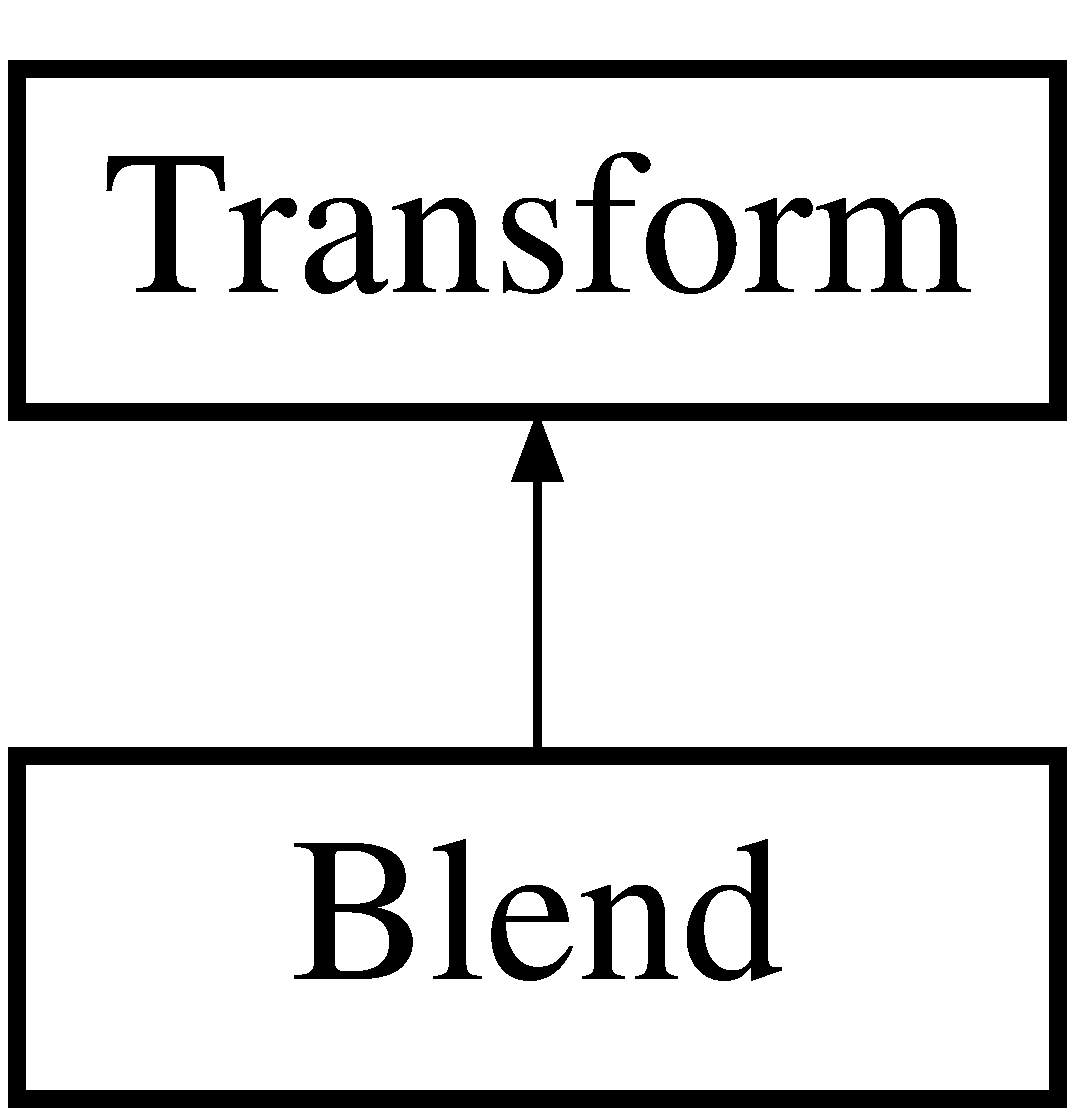
\includegraphics[height=2.000000cm]{class_blend}
\end{center}
\end{figure}
\subsection*{Public Member Functions}
\begin{DoxyCompactItemize}
\item 
\hypertarget{class_blend_a261679845165eb662efef8ce50cc0769}{}\label{class_blend_a261679845165eb662efef8ce50cc0769} 
{\bfseries Blend} (\hyperlink{class_color}{Color} input)
\item 
\hypertarget{class_blend_aea029e18e6b6daba142f0c785461e1ae}{}\label{class_blend_aea029e18e6b6daba142f0c785461e1ae} 
{\bfseries Blend} (double R, double G, double B)
\end{DoxyCompactItemize}
\subsection*{Additional Inherited Members}


The documentation for this class was generated from the following file\+:\begin{DoxyCompactItemize}
\item 
Transform.\+h\end{DoxyCompactItemize}

\hypertarget{class_box}{}\section{Box Class Reference}
\label{class_box}\index{Box@{Box}}


The basic building block for the game.  




{\ttfamily \#include $<$Scr\+Obj.\+h$>$}

Inheritance diagram for Box\+:\begin{figure}[H]
\begin{center}
\leavevmode
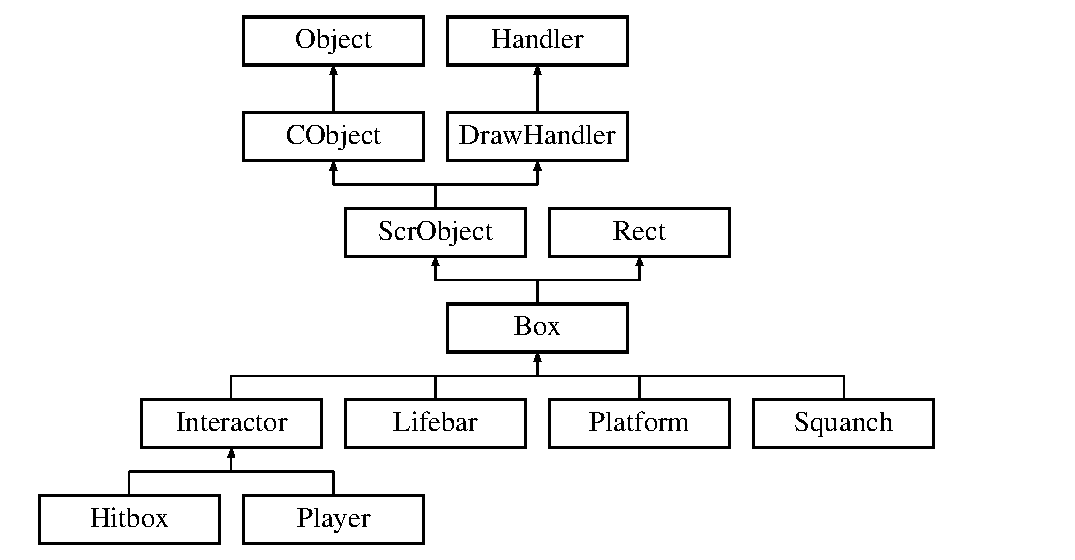
\includegraphics[height=6.000000cm]{class_box}
\end{center}
\end{figure}
\subsection*{Public Member Functions}
\begin{DoxyCompactItemize}
\item 
\hypertarget{class_box_a1a76055740b6ae3061ae210cd55785b7}{}\label{class_box_a1a76055740b6ae3061ae210cd55785b7} 
{\bfseries Box} (class \hyperlink{class_engine}{Engine} $\ast$game, \hyperlink{class_rect}{Rect} refrect)
\item 
\hypertarget{class_box_a97fa7330aafa9f4cafe300cbf3436d04}{}\label{class_box_a97fa7330aafa9f4cafe300cbf3436d04} 
void {\bfseries Draw\+Event} (class \hyperlink{class_engine}{Engine} $\ast$game\+Engine, \hyperlink{class_transform}{Transform} parent\+Trans)
\end{DoxyCompactItemize}
\subsection*{Additional Inherited Members}


\subsection{Detailed Description}
The basic building block for the game. 

Combining Screen \hyperlink{class_object}{Object} and \hyperlink{class_rect}{Rect}, this class represents an object that can be drawn on the screen, with its reference space being used to both draw and calculate bounding box collisions. Its overload of the Draw\+Event method stretches its associated Objects to fit its \hyperlink{class_rect}{Rect}\textquotesingle{}s reference space. (after any other transformations supplied to the object, which allows for \char`\"{}stretching\char`\"{} that doesn\textquotesingle{}t match exactly the \hyperlink{class_rect}{Rect}\textquotesingle{}s reference space) 

The documentation for this class was generated from the following files\+:\begin{DoxyCompactItemize}
\item 
Scr\+Obj.\+h\item 
Scr\+Obj.\+cpp\end{DoxyCompactItemize}

\hypertarget{class_camera}{}\section{Camera Class Reference}
\label{class_camera}\index{Camera@{Camera}}
\subsection*{Public Member Functions}
\begin{DoxyCompactItemize}
\item 
\hypertarget{class_camera_a58e5645c8597e4835aa55efdb289a7db}{}\label{class_camera_a58e5645c8597e4835aa55efdb289a7db} 
{\bfseries Camera} (float field\+Of\+View, float aspect\+Ratio, float z\+Near, float z\+Far, float x\+Pos, float y\+Pos, float z\+Pos)
\item 
\hypertarget{class_camera_aa67fdde5001bb777ad917c3a1a40fd60}{}\label{class_camera_aa67fdde5001bb777ad917c3a1a40fd60} 
void {\bfseries update\+Camera} ()
\item 
\hypertarget{class_camera_ad97a8d5eab9961181e7d96315f5938c6}{}\label{class_camera_ad97a8d5eab9961181e7d96315f5938c6} 
glm\+::mat4 {\bfseries get\+Projection} ()
\end{DoxyCompactItemize}


The documentation for this class was generated from the following files\+:\begin{DoxyCompactItemize}
\item 
Camera.\+h\item 
Camera.\+cpp\end{DoxyCompactItemize}

\hypertarget{class_c_object}{}\section{C\+Object Class Reference}
\label{class_c_object}\index{C\+Object@{C\+Object}}


C\+O\+L\+L\+E\+C\+T\+I\+ON O\+B\+J\+E\+CT Basic building block for your game objects. Tiles inherit from this, and most if not all game objects should inherit from this.  




{\ttfamily \#include $<$C\+Object.\+h$>$}

Inheritance diagram for C\+Object\+:\begin{figure}[H]
\begin{center}
\leavevmode
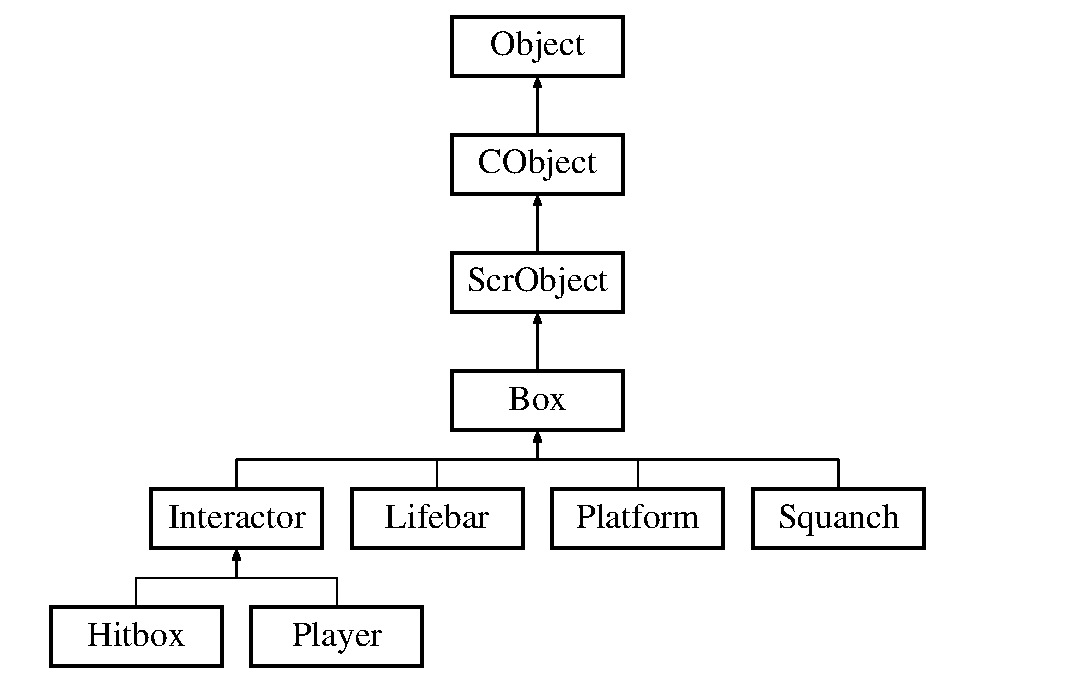
\includegraphics[height=6.000000cm]{class_c_object}
\end{center}
\end{figure}
\subsection*{Public Member Functions}
\begin{DoxyCompactItemize}
\item 
\hypertarget{class_c_object_ac44111d5ac75248a616df61b038c4153}{}\label{class_c_object_ac44111d5ac75248a616df61b038c4153} 
\hyperlink{class_c_object_ac44111d5ac75248a616df61b038c4153}{C\+Object} ()
\begin{DoxyCompactList}\small\item\em Empty constructor. \end{DoxyCompactList}\item 
\hypertarget{class_c_object_a93a3c3bc7d9a6462ef00e25404d9b0eb}{}\label{class_c_object_a93a3c3bc7d9a6462ef00e25404d9b0eb} 
\hyperlink{class_c_object_a93a3c3bc7d9a6462ef00e25404d9b0eb}{$\sim$\+C\+Object} ()
\begin{DoxyCompactList}\small\item\em Empty destructor. \end{DoxyCompactList}\item 
virtual void \hyperlink{class_c_object_a65338dd4ac20a20340875597344c0c4b}{Draw} (class \hyperlink{class_engine}{Engine} $\ast$game\+Engine, \hyperlink{class_transform}{Transform} parent\+Trans)
\begin{DoxyCompactList}\small\item\em Calls draw on all the objects in the collection, while passing transform information down. The game programmer will rarely (never) explicitly call a specific \hyperlink{class_c_object}{C\+Object}\textquotesingle{}s Draw since this is mainly for passing transform information down. \end{DoxyCompactList}\end{DoxyCompactItemize}
\subsection*{Public Attributes}
\begin{DoxyCompactItemize}
\item 
\hypertarget{class_c_object_a3248fbe274d6d69f38fccb60fdd5ceb3}{}\label{class_c_object_a3248fbe274d6d69f38fccb60fdd5ceb3} 
\hyperlink{class_obj_collection}{Obj\+Collection} \hyperlink{class_c_object_a3248fbe274d6d69f38fccb60fdd5ceb3}{my\+Stuff}
\begin{DoxyCompactList}\small\item\em The collection of objects associated with this \hyperlink{class_c_object}{C\+Object}. \end{DoxyCompactList}\end{DoxyCompactItemize}


\subsection{Detailed Description}
C\+O\+L\+L\+E\+C\+T\+I\+ON O\+B\+J\+E\+CT Basic building block for your game objects. Tiles inherit from this, and most if not all game objects should inherit from this. 

A \hyperlink{class_c_object}{C\+Object}\textquotesingle{}s (Collection \hyperlink{class_object}{Object}) job is to store other objects/\+C\+Objects and pass down transformation info down the object chain. They can be used to group different kinds of objects, for example, and easily transform the group as a whole while conforming to parent reference transforms. 

\subsection{Member Function Documentation}
\hypertarget{class_c_object_a65338dd4ac20a20340875597344c0c4b}{}\label{class_c_object_a65338dd4ac20a20340875597344c0c4b} 
\index{C\+Object@{C\+Object}!Draw@{Draw}}
\index{Draw@{Draw}!C\+Object@{C\+Object}}
\subsubsection{\texorpdfstring{Draw()}{Draw()}}
{\footnotesize\ttfamily void C\+Object\+::\+Draw (\begin{DoxyParamCaption}\item[{class \hyperlink{class_engine}{Engine} $\ast$}]{game\+Engine,  }\item[{\hyperlink{class_transform}{Transform}}]{parent\+Trans }\end{DoxyParamCaption})\hspace{0.3cm}{\ttfamily [virtual]}}



Calls draw on all the objects in the collection, while passing transform information down. The game programmer will rarely (never) explicitly call a specific \hyperlink{class_c_object}{C\+Object}\textquotesingle{}s Draw since this is mainly for passing transform information down. 


\begin{DoxyParams}{Parameters}
{\em game\+Engine} & -\/ pointer to engine that will draw this collection \\
\hline
{\em parent\+Trans} & -\/ transform information being applied to objects in this collection \\
\hline
\end{DoxyParams}


Implements \hyperlink{class_object_adeb7a19aaca51dbf093b37fd21c5e41f}{Object}.



The documentation for this class was generated from the following files\+:\begin{DoxyCompactItemize}
\item 
C\+Object.\+h\item 
C\+Object.\+cpp\end{DoxyCompactItemize}

\hypertarget{class_color}{}\section{Color Class Reference}
\label{class_color}\index{Color@{Color}}
\subsection*{Public Member Functions}
\begin{DoxyCompactItemize}
\item 
\hypertarget{class_color_ae0541336b70cced03c2c45a3a2b7b354}{}\label{class_color_ae0541336b70cced03c2c45a3a2b7b354} 
{\bfseries Color} (double R, double G, double B)
\item 
\hypertarget{class_color_ab8a27fb7806f0463f81779a727b10d53}{}\label{class_color_ab8a27fb7806f0463f81779a727b10d53} 
{\bfseries Color} (const \hyperlink{class_color}{Color} \&thing)
\item 
\hypertarget{class_color_a279277fa3deb3c47ea73b87cbb284d30}{}\label{class_color_a279277fa3deb3c47ea73b87cbb284d30} 
\hyperlink{class_color}{Color} \& {\bfseries operator=} (const \hyperlink{class_color}{Color} \&thing)
\end{DoxyCompactItemize}
\subsection*{Public Attributes}
\begin{DoxyCompactItemize}
\item 
\hypertarget{class_color_a12b28b8a60c6add344b485d12e1d2168}{}\label{class_color_a12b28b8a60c6add344b485d12e1d2168} 
double {\bfseries r}
\item 
\hypertarget{class_color_adcc846eae0491cee6a64f503044bca1b}{}\label{class_color_adcc846eae0491cee6a64f503044bca1b} 
double {\bfseries g}
\item 
\hypertarget{class_color_a37683f9d882695ac49f945d52158055a}{}\label{class_color_a37683f9d882695ac49f945d52158055a} 
double {\bfseries b}
\end{DoxyCompactItemize}


The documentation for this class was generated from the following files\+:\begin{DoxyCompactItemize}
\item 
Color.\+h\item 
Color.\+cpp\end{DoxyCompactItemize}

\hypertarget{class_draw_handler}{}\section{Draw\+Handler Class Reference}
\label{class_draw_handler}\index{Draw\+Handler@{Draw\+Handler}}
Inheritance diagram for Draw\+Handler\+:\begin{figure}[H]
\begin{center}
\leavevmode
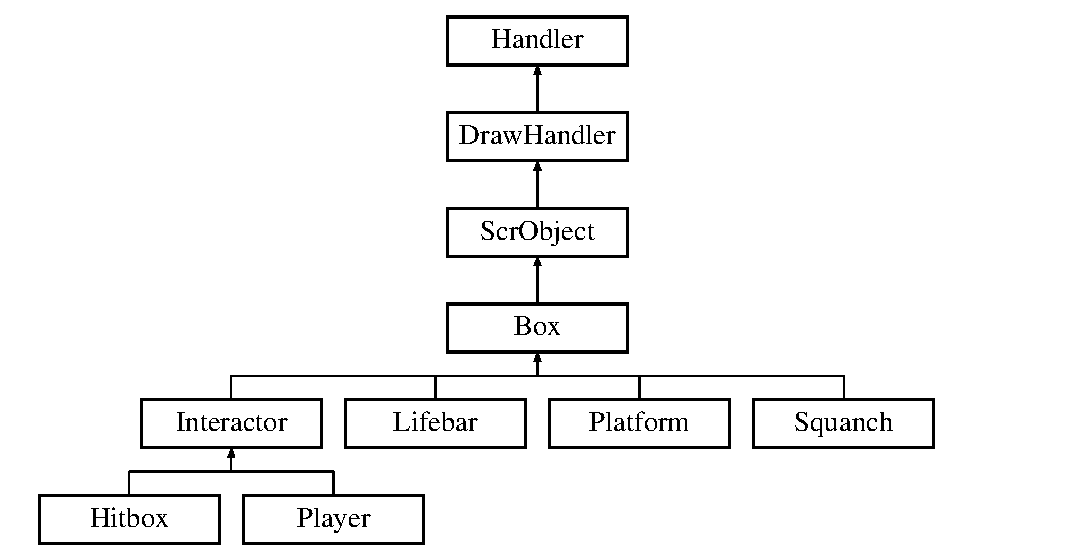
\includegraphics[height=6.000000cm]{class_draw_handler}
\end{center}
\end{figure}
\subsection*{Public Member Functions}
\begin{DoxyCompactItemize}
\item 
\hypertarget{class_draw_handler_a4bb69706083b6813cadfda8d3f7e0806}{}\label{class_draw_handler_a4bb69706083b6813cadfda8d3f7e0806} 
{\bfseries Draw\+Handler} (class \hyperlink{class_engine}{Engine} $\ast$game)
\item 
\hypertarget{class_draw_handler_a6ea4ba475a611834760c4dd5bb7313fe}{}\label{class_draw_handler_a6ea4ba475a611834760c4dd5bb7313fe} 
virtual void {\bfseries Draw\+Event} (class \hyperlink{class_engine}{Engine} $\ast$game\+Engine, \hyperlink{class_transform}{Transform} parent\+Trans)=0
\end{DoxyCompactItemize}
\subsection*{Additional Inherited Members}


The documentation for this class was generated from the following files\+:\begin{DoxyCompactItemize}
\item 
Handler.\+h\item 
Handler.\+cpp\end{DoxyCompactItemize}

\hypertarget{class_engine}{}\section{Engine Class Reference}
\label{class_engine}\index{Engine@{Engine}}


Game engine class. Not meant to be derived from.  




{\ttfamily \#include $<$Engine.\+h$>$}

\subsection*{Public Member Functions}
\begin{DoxyCompactItemize}
\item 
\hypertarget{class_engine_af4c789fb939a0870426c698a5124a0ee}{}\label{class_engine_af4c789fb939a0870426c698a5124a0ee} 
void {\bfseries Run} ()
\item 
\hypertarget{class_engine_a6eca7a961050e33cc3e801e8bd83baa4}{}\label{class_engine_a6eca7a961050e33cc3e801e8bd83baa4} 
double {\bfseries Get\+Time} ()
\item 
void \hyperlink{class_engine_a696e2de094fad8a043c105536a84754e}{Interact} (class \hyperlink{class_scr_object}{Scr\+Object} $\ast$obj)
\begin{DoxyCompactList}\small\item\em Method called by objects that want to interact with others. \end{DoxyCompactList}\item 
void \hyperlink{class_engine_a6636f2c1160776ebdcb1a07159c15e4a}{Udp\+Send} (\hyperlink{class_packet}{Packet} $\ast$pktin, \hyperlink{class_i_padd}{I\+Padd} addin, unsigned short portin)
\begin{DoxyCompactList}\small\item\em Basic networking method to send a packet. \end{DoxyCompactList}\item 
\hypertarget{class_engine_a6aaaa07c5d2706799deba2f29e88a2f7}{}\label{class_engine_a6aaaa07c5d2706799deba2f29e88a2f7} 
void \hyperlink{class_engine_a6aaaa07c5d2706799deba2f29e88a2f7}{Udp\+Bind} (unsigned short portin)
\begin{DoxyCompactList}\small\item\em Basic networking method to bind the engine\textquotesingle{}s socket to a port. \end{DoxyCompactList}\end{DoxyCompactItemize}
\subsection*{Public Attributes}
\begin{DoxyCompactItemize}
\item 
\hypertarget{class_engine_af71e99fa44783e7e43d54b1af786d219}{}\label{class_engine_af71e99fa44783e7e43d54b1af786d219} 
bool {\bfseries interact\+Entry}
\item 
\hypertarget{class_engine_ac6f3d9928c249b303891a2dff773637d}{}\label{class_engine_ac6f3d9928c249b303891a2dff773637d} 
sf\+::\+Udp\+Socket {\bfseries socket}
\item 
\hypertarget{class_engine_a5a108a01f06e9874ee4c1fda14ff03d8}{}\label{class_engine_a5a108a01f06e9874ee4c1fda14ff03d8} 
sf\+::\+Clock {\bfseries my\+Clock}
\item 
\hypertarget{class_engine_a82e2503954f7314236e0b50fa5019cd1}{}\label{class_engine_a82e2503954f7314236e0b50fa5019cd1} 
\hyperlink{class_camera}{Camera} {\bfseries my\+Cam}
\item 
\hypertarget{class_engine_ae7e9b4f9b0925005fb117dd1fadcfcfc}{}\label{class_engine_ae7e9b4f9b0925005fb117dd1fadcfcfc} 
sf\+::\+Window $\ast$ {\bfseries my\+Window}
\item 
\hypertarget{class_engine_ad0903c9fe548db11a3483f6dff106209}{}\label{class_engine_ad0903c9fe548db11a3483f6dff106209} 
\hyperlink{class_split_shader}{Split\+Shader} {\bfseries shader}
\item 
\hypertarget{class_engine_ab65a6d60cc6723aa970b42f254f8afbd}{}\label{class_engine_ab65a6d60cc6723aa970b42f254f8afbd} 
\hyperlink{class_split_shader_t_x}{Split\+Shader\+TX} {\bfseries T\+Xshader}
\item 
\hypertarget{class_engine_ab52c953691910ddd4b362e1991f8535b}{}\label{class_engine_ab52c953691910ddd4b362e1991f8535b} 
\hyperlink{class_handler_collection}{Handler\+Collection} {\bfseries time\+Handlers}
\item 
\hypertarget{class_engine_a022168a4bc78cd2b4e09066ce8491810}{}\label{class_engine_a022168a4bc78cd2b4e09066ce8491810} 
\hyperlink{class_handler_collection}{Handler\+Collection} {\bfseries key\+Handlers}
\item 
\hypertarget{class_engine_a7591342e66411592267969adb4902e07}{}\label{class_engine_a7591342e66411592267969adb4902e07} 
\hyperlink{class_handler_collection}{Handler\+Collection} {\bfseries draw\+Handlers}
\item 
\hypertarget{class_engine_a37a58bbf99c4f9f8be327703af07d546}{}\label{class_engine_a37a58bbf99c4f9f8be327703af07d546} 
\hyperlink{class_handler_collection}{Handler\+Collection} {\bfseries interact\+Handlers}
\item 
\hypertarget{class_engine_ac693cf7cd72cdce149af50599c841440}{}\label{class_engine_ac693cf7cd72cdce149af50599c841440} 
\hyperlink{class_handler_collection}{Handler\+Collection} {\bfseries network\+Handlers}
\end{DoxyCompactItemize}


\subsection{Detailed Description}
Game engine class. Not meant to be derived from. 

The game engine must first be created and then populated with objects before it is Run(). It manages the various game entities through its \hyperlink{class_handler}{Handler} collections. For example, all objects that are or have \hyperlink{class_draw_handler}{Draw\+Handler} are drawn in the \hyperlink{class_engine}{Engine}\textquotesingle{}s update loop. When an object is created outside of the engine, it receives a pointer to the engine and populates the respective collections on its own. 

\subsection{Member Function Documentation}
\hypertarget{class_engine_a696e2de094fad8a043c105536a84754e}{}\label{class_engine_a696e2de094fad8a043c105536a84754e} 
\index{Engine@{Engine}!Interact@{Interact}}
\index{Interact@{Interact}!Engine@{Engine}}
\subsubsection{\texorpdfstring{Interact()}{Interact()}}
{\footnotesize\ttfamily void Engine\+::\+Interact (\begin{DoxyParamCaption}\item[{class \hyperlink{class_scr_object}{Scr\+Object} $\ast$}]{obj }\end{DoxyParamCaption})}



Method called by objects that want to interact with others. 


\begin{DoxyParams}{Parameters}
{\em obj} & -\/ The object calling this method must pass itself as an argument. \\
\hline
\end{DoxyParams}
\hypertarget{class_engine_a6636f2c1160776ebdcb1a07159c15e4a}{}\label{class_engine_a6636f2c1160776ebdcb1a07159c15e4a} 
\index{Engine@{Engine}!Udp\+Send@{Udp\+Send}}
\index{Udp\+Send@{Udp\+Send}!Engine@{Engine}}
\subsubsection{\texorpdfstring{Udp\+Send()}{UdpSend()}}
{\footnotesize\ttfamily void Engine\+::\+Udp\+Send (\begin{DoxyParamCaption}\item[{\hyperlink{class_packet}{Packet} $\ast$}]{pktin,  }\item[{\hyperlink{class_i_padd}{I\+Padd}}]{addin,  }\item[{unsigned short}]{portin }\end{DoxyParamCaption})}



Basic networking method to send a packet. 


\begin{DoxyParams}{Parameters}
{\em pktin} & -\/ Pointer to the packet being sent. \\
\hline
{\em \hyperlink{class_i_padd}{I\+Padd}} & -\/ IP address of recipient; \\
\hline
{\em portin} & -\/ Port of recipient. \\
\hline
\end{DoxyParams}


The documentation for this class was generated from the following files\+:\begin{DoxyCompactItemize}
\item 
Engine.\+h\item 
Engine.\+cpp\end{DoxyCompactItemize}

\hypertarget{class_fancy_square}{}\section{Fancy\+Square Class Reference}
\label{class_fancy_square}\index{Fancy\+Square@{Fancy\+Square}}


Low-\/level \hyperlink{class_object}{Object} prefab that draws a simple textured square.  




{\ttfamily \#include $<$Shape.\+h$>$}

Inheritance diagram for Fancy\+Square\+:\begin{figure}[H]
\begin{center}
\leavevmode
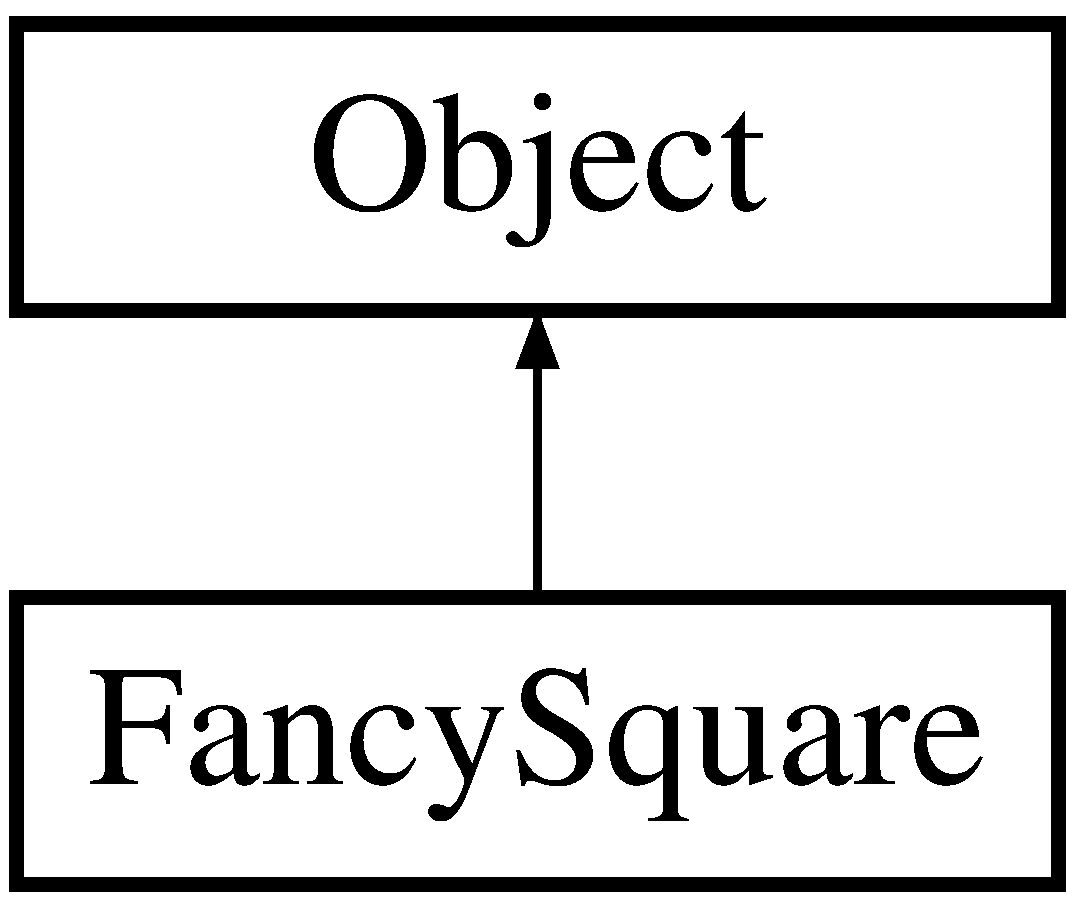
\includegraphics[height=2.000000cm]{class_fancy_square}
\end{center}
\end{figure}
\subsection*{Public Member Functions}
\begin{DoxyCompactItemize}
\item 
\hypertarget{class_fancy_square_a2ddb3b7be2421b2f6753ed6bb747f2ea}{}\label{class_fancy_square_a2ddb3b7be2421b2f6753ed6bb747f2ea} 
{\bfseries Fancy\+Square} (const char $\ast$input)
\item 
virtual void \hyperlink{class_fancy_square_ac77d35ba8ab766f8a3e35f68e7344953}{Draw} (class \hyperlink{class_engine}{Engine} $\ast$game\+Engine, \hyperlink{class_transform}{Transform} parent\+Trans)
\begin{DoxyCompactList}\small\item\em Virtual function meant to be implemented by children. Some objects use Draw to pass information, delegating the actual drawing to the objects at the end of the parent-\/child hierarchy. \end{DoxyCompactList}\end{DoxyCompactItemize}
\subsection*{Public Attributes}
\begin{DoxyCompactItemize}
\item 
\hypertarget{class_fancy_square_ae08622ddfab2e5c59a2af7978b10b0fc}{}\label{class_fancy_square_ae08622ddfab2e5c59a2af7978b10b0fc} 
\hyperlink{class_split_model_t_x}{Split\+Model\+TX} {\bfseries my\+Obj}
\end{DoxyCompactItemize}


\subsection{Detailed Description}
Low-\/level \hyperlink{class_object}{Object} prefab that draws a simple textured square. 

\subsection{Member Function Documentation}
\hypertarget{class_fancy_square_ac77d35ba8ab766f8a3e35f68e7344953}{}\label{class_fancy_square_ac77d35ba8ab766f8a3e35f68e7344953} 
\index{Fancy\+Square@{Fancy\+Square}!Draw@{Draw}}
\index{Draw@{Draw}!Fancy\+Square@{Fancy\+Square}}
\subsubsection{\texorpdfstring{Draw()}{Draw()}}
{\footnotesize\ttfamily void Fancy\+Square\+::\+Draw (\begin{DoxyParamCaption}\item[{class \hyperlink{class_engine}{Engine} $\ast$}]{game\+Engine,  }\item[{\hyperlink{class_transform}{Transform}}]{parent\+Trans }\end{DoxyParamCaption})\hspace{0.3cm}{\ttfamily [virtual]}}



Virtual function meant to be implemented by children. Some objects use Draw to pass information, delegating the actual drawing to the objects at the end of the parent-\/child hierarchy. 


\begin{DoxyParams}{Parameters}
{\em game\+Engine} & -\/ Pointer to the game engine that will render this \\
\hline
{\em parent\+Trans} & -\/ \hyperlink{class_transform}{Transform} being passed to the object. With long chains of object children/parents, transforms can be cumulative. \\
\hline
\end{DoxyParams}


Implements \hyperlink{class_object_adeb7a19aaca51dbf093b37fd21c5e41f}{Object}.



The documentation for this class was generated from the following files\+:\begin{DoxyCompactItemize}
\item 
Shape.\+h\item 
Shape.\+cpp\end{DoxyCompactItemize}

\hypertarget{class_handler}{}\section{Handler Class Reference}
\label{class_handler}\index{Handler@{Handler}}


Base class for the game\textquotesingle{}s event handlers.  




{\ttfamily \#include $<$Handler.\+h$>$}

Inheritance diagram for Handler\+:\begin{figure}[H]
\begin{center}
\leavevmode
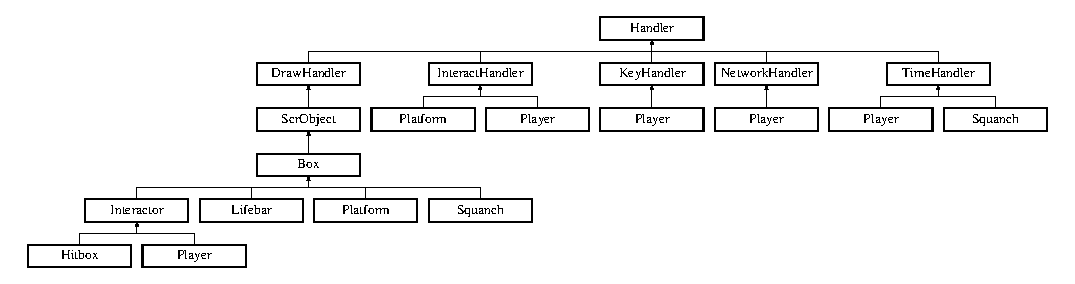
\includegraphics[height=3.363363cm]{class_handler}
\end{center}
\end{figure}
\subsection*{Public Member Functions}
\begin{DoxyCompactItemize}
\item 
\hypertarget{class_handler_a65054f56eca474ad58a12067347d341c}{}\label{class_handler_a65054f56eca474ad58a12067347d341c} 
{\bfseries Handler} (class \hyperlink{class_handler_collection}{Handler\+Collection} $\ast$input)
\item 
\hypertarget{class_handler_a1d7568b0690d98cfecf0b446de9c4250}{}\label{class_handler_a1d7568b0690d98cfecf0b446de9c4250} 
void {\bfseries Hold} (class \hyperlink{class_handler_collection}{Handler\+Collection} $\ast$target)
\item 
\hypertarget{class_handler_aaccb98d642889447dc7d8645df9ef773}{}\label{class_handler_aaccb98d642889447dc7d8645df9ef773} 
void {\bfseries Letgo} ()
\end{DoxyCompactItemize}
\subsection*{Public Attributes}
\begin{DoxyCompactItemize}
\item 
\hypertarget{class_handler_a439521850c1d2a5bed66ad4e878bb5ca}{}\label{class_handler_a439521850c1d2a5bed66ad4e878bb5ca} 
class \hyperlink{class_handler_collection}{Handler\+Collection} $\ast$ {\bfseries my\+Collection}
\item 
\hypertarget{class_handler_acee999ed1680b7e1d3c71def7570d864}{}\label{class_handler_acee999ed1680b7e1d3c71def7570d864} 
struct \hyperlink{struct_hand_ls_node}{Hand\+Ls\+Node} $\ast$ {\bfseries my\+Node}
\end{DoxyCompactItemize}


\subsection{Detailed Description}
Base class for the game\textquotesingle{}s event handlers. 

This engine processes events instead of having predefined code in an update loop. Objects that trigger or listen for events will normally inherit from either \hyperlink{class_time_handler}{Time\+Handler} or Keyhandler, and then implement the abstract functions. \hyperlink{class_key_handler}{Key\+Handler} has an enum interface that works with S\+F\+ML, while the \hyperlink{class_engine}{Engine} has a clock that works for \hyperlink{class_time_handler}{Time\+Handler}. Objects that want to be interacted with must inherit from or have an \hyperlink{class_interact_handler}{Interact\+Handler}. To be drawn by the engine, objects must be Draw\+Handlers. 

The documentation for this class was generated from the following files\+:\begin{DoxyCompactItemize}
\item 
Handler.\+h\item 
Handler.\+cpp\end{DoxyCompactItemize}

\hypertarget{class_handler_collection}{}\section{Handler\+Collection Class Reference}
\label{class_handler_collection}\index{Handler\+Collection@{Handler\+Collection}}
\subsection*{Public Member Functions}
\begin{DoxyCompactItemize}
\item 
\hypertarget{class_handler_collection_addbedfb20eb3cf420181d24cdf637e04}{}\label{class_handler_collection_addbedfb20eb3cf420181d24cdf637e04} 
\hyperlink{struct_hand_ls_node}{Hand\+Ls\+Node} $\ast$ {\bfseries Add} (\hyperlink{class_handler}{Handler} $\ast$in\+Handler)
\item 
\hypertarget{class_handler_collection_af12bcbf2f10f593abcf11ef36b22036d}{}\label{class_handler_collection_af12bcbf2f10f593abcf11ef36b22036d} 
void {\bfseries Remove} (\hyperlink{struct_hand_ls_node}{Hand\+Ls\+Node} $\ast$target)
\item 
\hypertarget{class_handler_collection_a63a6d4616f0410f8e9c5b3d2965a424b}{}\label{class_handler_collection_a63a6d4616f0410f8e9c5b3d2965a424b} 
\hyperlink{struct_hand_ls_node}{Hand\+Ls\+Node} $\ast$ {\bfseries Get\+First} ()
\item 
\hypertarget{class_handler_collection_a0ef8229aa3a1591351897dded37cd07e}{}\label{class_handler_collection_a0ef8229aa3a1591351897dded37cd07e} 
\hyperlink{struct_hand_ls_node}{Hand\+Ls\+Node} $\ast$ {\bfseries Get\+Next} ()
\end{DoxyCompactItemize}
\subsection*{Public Attributes}
\begin{DoxyCompactItemize}
\item 
\hypertarget{class_handler_collection_abf67414e513553827caa3664675224b7}{}\label{class_handler_collection_abf67414e513553827caa3664675224b7} 
\hyperlink{struct_hand_ls_node}{Hand\+Ls\+Node} $\ast$ {\bfseries my\+Head}
\item 
\hypertarget{class_handler_collection_a86ad3cf7be660dfad3c6e7bfc6ed31a8}{}\label{class_handler_collection_a86ad3cf7be660dfad3c6e7bfc6ed31a8} 
\hyperlink{struct_hand_ls_node}{Hand\+Ls\+Node} $\ast$ {\bfseries curr\+Ptr}
\end{DoxyCompactItemize}


The documentation for this class was generated from the following files\+:\begin{DoxyCompactItemize}
\item 
Handler\+Collection.\+h\item 
Handler\+Collection.\+cpp\end{DoxyCompactItemize}

\hypertarget{struct_hand_ls_node}{}\section{Hand\+Ls\+Node Struct Reference}
\label{struct_hand_ls_node}\index{Hand\+Ls\+Node@{Hand\+Ls\+Node}}
\subsection*{Public Member Functions}
\begin{DoxyCompactItemize}
\item 
\hypertarget{struct_hand_ls_node_a569a10760d13333ed184aedc0104ff26}{}\label{struct_hand_ls_node_a569a10760d13333ed184aedc0104ff26} 
{\bfseries Hand\+Ls\+Node} (\hyperlink{class_handler}{Handler} $\ast$in\+Handler)
\end{DoxyCompactItemize}
\subsection*{Public Attributes}
\begin{DoxyCompactItemize}
\item 
\hypertarget{struct_hand_ls_node_a0e8014f915df2512d0ad44f32003d710}{}\label{struct_hand_ls_node_a0e8014f915df2512d0ad44f32003d710} 
\hyperlink{class_handler}{Handler} $\ast$ {\bfseries my\+Handler}
\item 
\hypertarget{struct_hand_ls_node_a38ea26d6ddfa4170763bad9d06d435bb}{}\label{struct_hand_ls_node_a38ea26d6ddfa4170763bad9d06d435bb} 
\hyperlink{struct_hand_ls_node}{Hand\+Ls\+Node} $\ast$ {\bfseries next\+Node}
\item 
\hypertarget{struct_hand_ls_node_a6e42f95e93458d11cb562d3d986f6733}{}\label{struct_hand_ls_node_a6e42f95e93458d11cb562d3d986f6733} 
\hyperlink{struct_hand_ls_node}{Hand\+Ls\+Node} $\ast$ {\bfseries prev\+Node}
\end{DoxyCompactItemize}


The documentation for this struct was generated from the following file\+:\begin{DoxyCompactItemize}
\item 
Handler\+Collection.\+h\end{DoxyCompactItemize}

\hypertarget{class_hitbox}{}\section{Hitbox Class Reference}
\label{class_hitbox}\index{Hitbox@{Hitbox}}
Inheritance diagram for Hitbox\+:\begin{figure}[H]
\begin{center}
\leavevmode
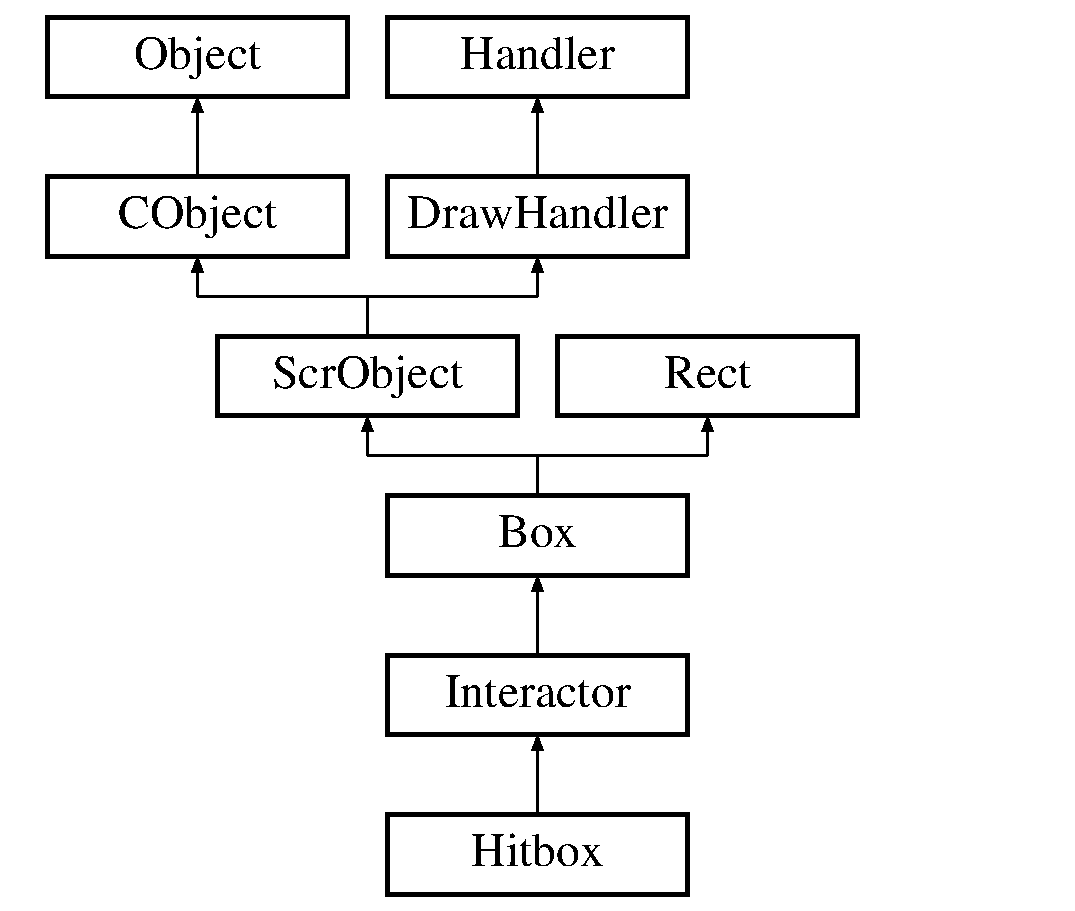
\includegraphics[height=6.000000cm]{class_hitbox}
\end{center}
\end{figure}
\subsection*{Public Member Functions}
\begin{DoxyCompactItemize}
\item 
\hypertarget{class_hitbox_a986c9a4829e3ce01e590ffdfe5835699}{}\label{class_hitbox_a986c9a4829e3ce01e590ffdfe5835699} 
{\bfseries Hitbox} (\hyperlink{class_engine}{Engine} $\ast$game, \hyperlink{class_rect}{Rect} refrect, class \hyperlink{class_player}{Player} $\ast$in)
\item 
\hypertarget{class_hitbox_a4885229ccba5a16403919055e8778923}{}\label{class_hitbox_a4885229ccba5a16403919055e8778923} 
void {\bfseries Interact\+Player} (class \hyperlink{class_player}{Player} $\ast$other)
\end{DoxyCompactItemize}
\subsection*{Public Attributes}
\begin{DoxyCompactItemize}
\item 
\hypertarget{class_hitbox_ab3d848f9286164ba8cbb6a85c441d0f5}{}\label{class_hitbox_ab3d848f9286164ba8cbb6a85c441d0f5} 
class \hyperlink{class_player}{Player} $\ast$ {\bfseries me}
\end{DoxyCompactItemize}


The documentation for this class was generated from the following file\+:\begin{DoxyCompactItemize}
\item 
Fight\+Game.\+cpp\end{DoxyCompactItemize}

\hypertarget{class_identity}{}\section{Identity Class Reference}
\label{class_identity}\index{Identity@{Identity}}
Inheritance diagram for Identity\+:\begin{figure}[H]
\begin{center}
\leavevmode
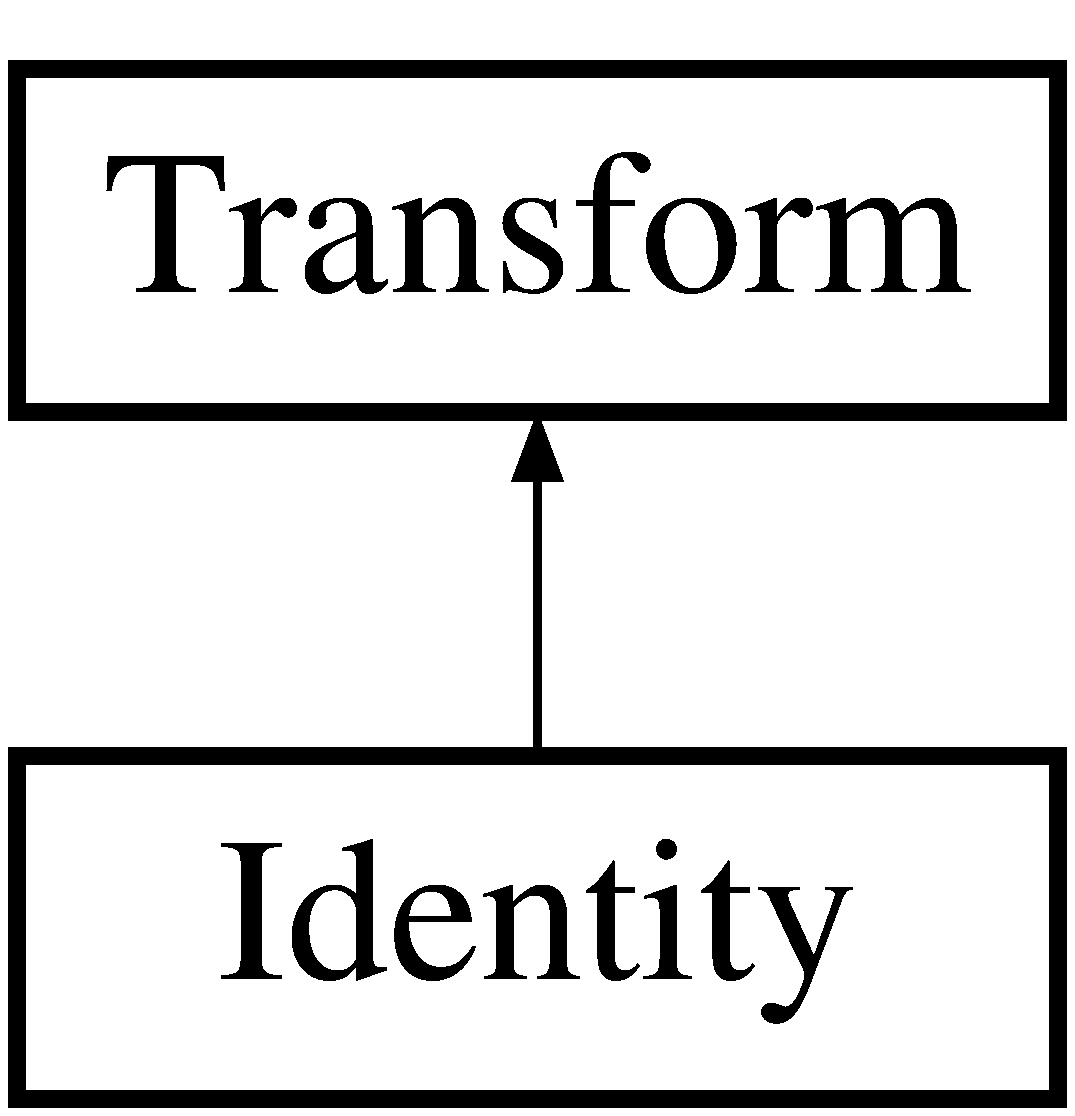
\includegraphics[height=2.000000cm]{class_identity}
\end{center}
\end{figure}
\subsection*{Additional Inherited Members}


The documentation for this class was generated from the following file\+:\begin{DoxyCompactItemize}
\item 
Transform.\+h\end{DoxyCompactItemize}

\hypertarget{class_interact_handler}{}\section{Interact\+Handler Class Reference}
\label{class_interact_handler}\index{Interact\+Handler@{Interact\+Handler}}
Inheritance diagram for Interact\+Handler\+:\begin{figure}[H]
\begin{center}
\leavevmode
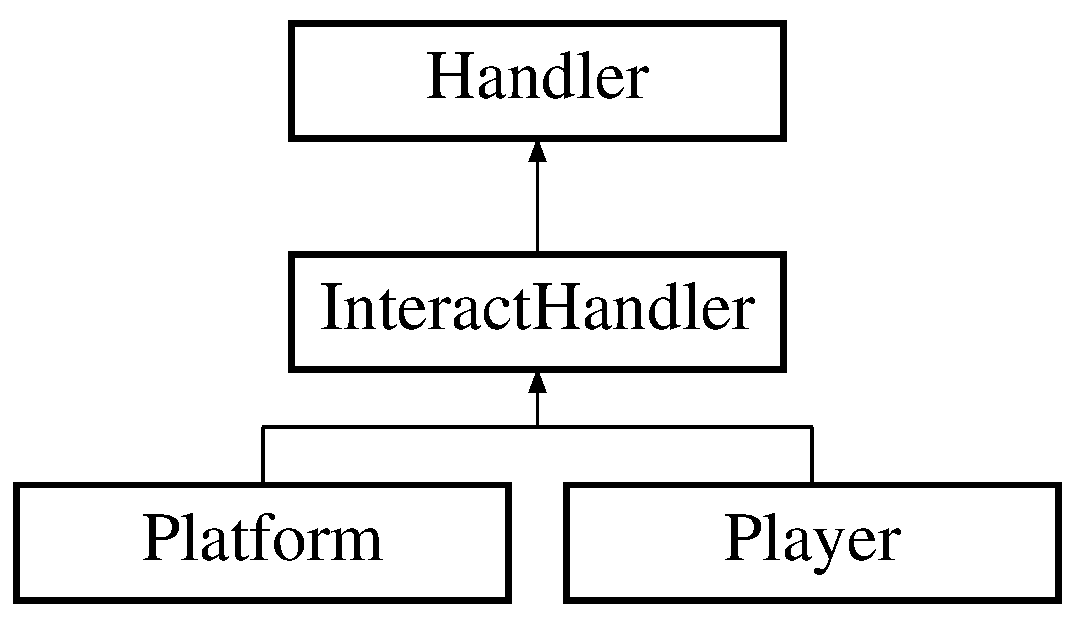
\includegraphics[height=3.000000cm]{class_interact_handler}
\end{center}
\end{figure}
\subsection*{Public Member Functions}
\begin{DoxyCompactItemize}
\item 
\hypertarget{class_interact_handler_a7a5a23fb8b7ab66282fa7e9e7f5f6004}{}\label{class_interact_handler_a7a5a23fb8b7ab66282fa7e9e7f5f6004} 
{\bfseries Interact\+Handler} (class \hyperlink{class_engine}{Engine} $\ast$game)
\item 
\hypertarget{class_interact_handler_a3c493434e2cd4e5b9ca4843005ed73cb}{}\label{class_interact_handler_a3c493434e2cd4e5b9ca4843005ed73cb} 
virtual void {\bfseries Interact\+Event} (class \hyperlink{class_scr_object}{Scr\+Object} $\ast$obj)=0
\end{DoxyCompactItemize}
\subsection*{Additional Inherited Members}


The documentation for this class was generated from the following files\+:\begin{DoxyCompactItemize}
\item 
Handler.\+h\item 
Handler.\+cpp\end{DoxyCompactItemize}

\hypertarget{class_interactor}{}\section{Interactor Class Reference}
\label{class_interactor}\index{Interactor@{Interactor}}
Inheritance diagram for Interactor\+:\begin{figure}[H]
\begin{center}
\leavevmode
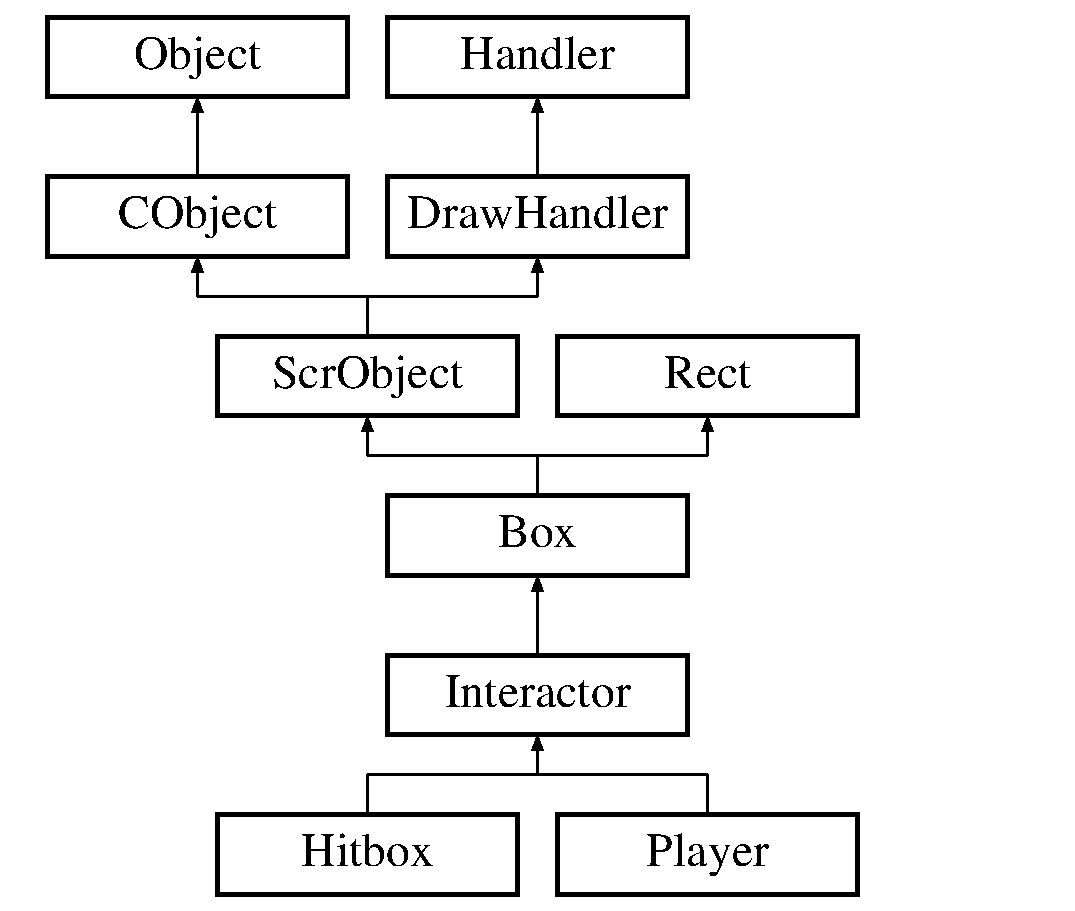
\includegraphics[height=6.000000cm]{class_interactor}
\end{center}
\end{figure}
\subsection*{Public Member Functions}
\begin{DoxyCompactItemize}
\item 
\hypertarget{class_interactor_afc2618cc8be769042fe84635f06baf14}{}\label{class_interactor_afc2618cc8be769042fe84635f06baf14} 
{\bfseries Interactor} (\hyperlink{class_engine}{Engine} $\ast$game, \hyperlink{class_rect}{Rect} refrect)
\item 
\hypertarget{class_interactor_a74fee5038189de32aae82d0358301b4b}{}\label{class_interactor_a74fee5038189de32aae82d0358301b4b} 
virtual void {\bfseries Interact\+Player} (class \hyperlink{class_player}{Player} $\ast$other)
\item 
\hypertarget{class_interactor_ae01bc3e9dcefe9e416b9da9d71cf4e82}{}\label{class_interactor_ae01bc3e9dcefe9e416b9da9d71cf4e82} 
virtual void {\bfseries Interact\+Platform} (class \hyperlink{class_platform}{Platform} $\ast$other)
\end{DoxyCompactItemize}
\subsection*{Public Attributes}
\begin{DoxyCompactItemize}
\item 
\hypertarget{class_interactor_a7349dd40ae48b78a4e491b41a373ba90}{}\label{class_interactor_a7349dd40ae48b78a4e491b41a373ba90} 
\hyperlink{class_engine}{Engine} $\ast$ {\bfseries gameptr}
\end{DoxyCompactItemize}


The documentation for this class was generated from the following file\+:\begin{DoxyCompactItemize}
\item 
Fight\+Game.\+cpp\end{DoxyCompactItemize}

\hypertarget{class_i_padd}{}\section{I\+Padd Class Reference}
\label{class_i_padd}\index{I\+Padd@{I\+Padd}}


Wrapper for sfml IP address class.  




{\ttfamily \#include $<$Network.\+h$>$}

\subsection*{Public Member Functions}
\begin{DoxyCompactItemize}
\item 
\hypertarget{class_i_padd_a1ab48dbb7feb2cacadeee14013b9c674}{}\label{class_i_padd_a1ab48dbb7feb2cacadeee14013b9c674} 
{\bfseries I\+Padd} (const char $\ast$input)
\item 
\hypertarget{class_i_padd_a239a6d6d6635bc580058d23ff32adf10}{}\label{class_i_padd_a239a6d6d6635bc580058d23ff32adf10} 
{\bfseries I\+Padd} (const \hyperlink{class_i_padd}{I\+Padd} \&input)
\item 
\hypertarget{class_i_padd_adbed9e60221ea1e5ac3464bfe17fdcf5}{}\label{class_i_padd_adbed9e60221ea1e5ac3464bfe17fdcf5} 
{\bfseries I\+Padd} (sf\+::\+Ip\+Address addin)
\item 
\hypertarget{class_i_padd_a19c791cae61178b0598fad23be2d0e8e}{}\label{class_i_padd_a19c791cae61178b0598fad23be2d0e8e} 
\hyperlink{class_i_padd}{I\+Padd} \& {\bfseries operator=} (const \hyperlink{class_i_padd}{I\+Padd} \&input)
\end{DoxyCompactItemize}
\subsection*{Public Attributes}
\begin{DoxyCompactItemize}
\item 
\hypertarget{class_i_padd_a4b9088ff481bb7c79e92e0d2f06faae1}{}\label{class_i_padd_a4b9088ff481bb7c79e92e0d2f06faae1} 
sf\+::\+Ip\+Address {\bfseries addr}
\end{DoxyCompactItemize}


\subsection{Detailed Description}
Wrapper for sfml IP address class. 

The documentation for this class was generated from the following files\+:\begin{DoxyCompactItemize}
\item 
Network.\+h\item 
Network.\+cpp\end{DoxyCompactItemize}

\hypertarget{class_key_handler_1_1_key}{}\section{Key\+Handler\+:\+:Key Class Reference}
\label{class_key_handler_1_1_key}\index{Key\+Handler\+::\+Key@{Key\+Handler\+::\+Key}}
\subsection*{Public Types}
\begin{DoxyCompactItemize}
\item 
enum \hyperlink{class_key_handler_1_1_key_a832541e186986ff9f6bd5a810ed5c164}{Keycode} \{ \newline
\hyperlink{class_key_handler_1_1_key_a832541e186986ff9f6bd5a810ed5c164ac80b99d4d6b9846fa39609c24217e58f}{Unknown} = -\/1, 
\hyperlink{class_key_handler_1_1_key_a832541e186986ff9f6bd5a810ed5c164a8efa41434e923f1a61d0f4b1a742c152}{A} = 0, 
\hyperlink{class_key_handler_1_1_key_a832541e186986ff9f6bd5a810ed5c164a64a868f2a3b899656eb605d7c5c832a1}{B}, 
\hyperlink{class_key_handler_1_1_key_a832541e186986ff9f6bd5a810ed5c164a07d7f0e4f3670ff07cd649a77c104b1e}{C}, 
\newline
\hyperlink{class_key_handler_1_1_key_a832541e186986ff9f6bd5a810ed5c164ac4f7283f592526f8aea5712037290fa7}{D}, 
\hyperlink{class_key_handler_1_1_key_a832541e186986ff9f6bd5a810ed5c164a8b651f8f29a7c804b53a0c160511ae49}{E}, 
\hyperlink{class_key_handler_1_1_key_a832541e186986ff9f6bd5a810ed5c164ad75a109842ef1ac7d07c3f6be865aeb7}{F}, 
\hyperlink{class_key_handler_1_1_key_a832541e186986ff9f6bd5a810ed5c164a54a78d1868d46882fdcfb65b92de7b91}{G}, 
\newline
\hyperlink{class_key_handler_1_1_key_a832541e186986ff9f6bd5a810ed5c164a3708fa0b0516fa1b3401a5044f7b212e}{H}, 
\hyperlink{class_key_handler_1_1_key_a832541e186986ff9f6bd5a810ed5c164ad15e0c59cd015691173e5cc6c48bd182}{I}, 
\hyperlink{class_key_handler_1_1_key_a832541e186986ff9f6bd5a810ed5c164a4ba5f406eadabb0d23b3e171fdd5f4eb}{J}, 
\hyperlink{class_key_handler_1_1_key_a832541e186986ff9f6bd5a810ed5c164a880cc51a91361c6c96c7f148213a8e75}{K}, 
\newline
\hyperlink{class_key_handler_1_1_key_a832541e186986ff9f6bd5a810ed5c164a67aba8d5780747863f750ee1fd4bad14}{L}, 
\hyperlink{class_key_handler_1_1_key_a832541e186986ff9f6bd5a810ed5c164a573ba33087bc1467fcf719dbc4d83b8b}{M}, 
\hyperlink{class_key_handler_1_1_key_a832541e186986ff9f6bd5a810ed5c164a1ab6d3767cb4f60f5b1be4f4794217af}{N}, 
\hyperlink{class_key_handler_1_1_key_a832541e186986ff9f6bd5a810ed5c164adaf8de28c483c61edcbbadea30117b17}{O}, 
\newline
\hyperlink{class_key_handler_1_1_key_a832541e186986ff9f6bd5a810ed5c164ae91576ccbb011bbb0e06ac3633ac9e34}{P}, 
\hyperlink{class_key_handler_1_1_key_a832541e186986ff9f6bd5a810ed5c164a4e68de6a49d6a34838fcd03ae92b7284}{Q}, 
\hyperlink{class_key_handler_1_1_key_a832541e186986ff9f6bd5a810ed5c164a1a14714229f65d75b8984fd0d23955c8}{R}, 
\hyperlink{class_key_handler_1_1_key_a832541e186986ff9f6bd5a810ed5c164a94493cabffa5bae30276eb354c3c552f}{S}, 
\newline
\hyperlink{class_key_handler_1_1_key_a832541e186986ff9f6bd5a810ed5c164a08c657ff499654c0408f613e23ed8f44}{T}, 
\hyperlink{class_key_handler_1_1_key_a832541e186986ff9f6bd5a810ed5c164adcb1b9cb0bb81da1e2fe82f3171938bd}{U}, 
\hyperlink{class_key_handler_1_1_key_a832541e186986ff9f6bd5a810ed5c164a80e8301fc2e1c0a329149bdf3015f9c2}{V}, 
\hyperlink{class_key_handler_1_1_key_a832541e186986ff9f6bd5a810ed5c164a1eee42314f265d55583b8575f9144404}{W}, 
\newline
\hyperlink{class_key_handler_1_1_key_a832541e186986ff9f6bd5a810ed5c164ae0f4fce5ae6792c9ebb49adedce9c5d4}{X}, 
\hyperlink{class_key_handler_1_1_key_a832541e186986ff9f6bd5a810ed5c164aaabfbd79d10faa782ad75b68b4c9564d}{Y}, 
\hyperlink{class_key_handler_1_1_key_a832541e186986ff9f6bd5a810ed5c164ac66f94fc7da9c1774e4233a440362f35}{Z}, 
\hyperlink{class_key_handler_1_1_key_a832541e186986ff9f6bd5a810ed5c164ab414103b554b09b25e27e67f22faac20}{Num0}, 
\newline
\hyperlink{class_key_handler_1_1_key_a832541e186986ff9f6bd5a810ed5c164a1910420bbcefbb463c827f95c8ec6a3f}{Num1}, 
\hyperlink{class_key_handler_1_1_key_a832541e186986ff9f6bd5a810ed5c164a1f317a1d4b5491948ca9c0c7ba1fef05}{Num2}, 
\hyperlink{class_key_handler_1_1_key_a832541e186986ff9f6bd5a810ed5c164a0ef0f9aa0ac92a70e19b104b51290eb5}{Num3}, 
\hyperlink{class_key_handler_1_1_key_a832541e186986ff9f6bd5a810ed5c164a14e1f6d0a80be11fc41a874e8e233120}{Num4}, 
\newline
\hyperlink{class_key_handler_1_1_key_a832541e186986ff9f6bd5a810ed5c164a5d2b8298858b094717c924e8909c9e31}{Num5}, 
\hyperlink{class_key_handler_1_1_key_a832541e186986ff9f6bd5a810ed5c164a1c50f6e0b15d3544261924ed4cbbb5ee}{Num6}, 
\hyperlink{class_key_handler_1_1_key_a832541e186986ff9f6bd5a810ed5c164a4f9a604ad40647b84ca8205663f2b263}{Num7}, 
\hyperlink{class_key_handler_1_1_key_a832541e186986ff9f6bd5a810ed5c164ad5260c696a6999de9998cb79b338fb56}{Num8}, 
\newline
\hyperlink{class_key_handler_1_1_key_a832541e186986ff9f6bd5a810ed5c164a0aeb972aa91160aa216a1cdc005fef48}{Num9}, 
\hyperlink{class_key_handler_1_1_key_a832541e186986ff9f6bd5a810ed5c164a303923da412dd7987f046dffe87cdb1d}{Escape}, 
\hyperlink{class_key_handler_1_1_key_a832541e186986ff9f6bd5a810ed5c164a97090e6da42c3b4c47eb134222826cc3}{L\+Control}, 
\hyperlink{class_key_handler_1_1_key_a832541e186986ff9f6bd5a810ed5c164a6273fc14747306032b36d43e6155df30}{L\+Shift}, 
\newline
\hyperlink{class_key_handler_1_1_key_a832541e186986ff9f6bd5a810ed5c164a3ac498d7a1ecb89ffb3d2a02a09303be}{L\+Alt}, 
\hyperlink{class_key_handler_1_1_key_a832541e186986ff9f6bd5a810ed5c164a2c7cae50215630f1da82446fe23e6994}{L\+System}, 
\hyperlink{class_key_handler_1_1_key_a832541e186986ff9f6bd5a810ed5c164aa288d5b4bff297b0642151d91e6be823}{R\+Control}, 
\hyperlink{class_key_handler_1_1_key_a832541e186986ff9f6bd5a810ed5c164a2021770abfe2d263856f7178ee3255cd}{R\+Shift}, 
\newline
\hyperlink{class_key_handler_1_1_key_a832541e186986ff9f6bd5a810ed5c164ad8fd531d243163f1c357729c3c137649}{R\+Alt}, 
\hyperlink{class_key_handler_1_1_key_a832541e186986ff9f6bd5a810ed5c164a976d46b2ae25030aa4ad9e9a5aed5cac}{R\+System}, 
\hyperlink{class_key_handler_1_1_key_a832541e186986ff9f6bd5a810ed5c164a4a77cac326e46de32f25ef1863a57a99}{Menu}, 
\hyperlink{class_key_handler_1_1_key_a832541e186986ff9f6bd5a810ed5c164a51d24046d4962e1e6877f1877913ba3c}{L\+Bracket}, 
\newline
\hyperlink{class_key_handler_1_1_key_a832541e186986ff9f6bd5a810ed5c164a08d13d228c5ceb776872a530307d8d9b}{R\+Bracket}, 
\hyperlink{class_key_handler_1_1_key_a832541e186986ff9f6bd5a810ed5c164afc4c701852a550c7ce608d5c1a8f74f4}{Semi\+Colon}, 
\hyperlink{class_key_handler_1_1_key_a832541e186986ff9f6bd5a810ed5c164acce12efa4af7b83362aea746009be3af}{Comma}, 
\hyperlink{class_key_handler_1_1_key_a832541e186986ff9f6bd5a810ed5c164afee555b1dffc60b2a14cf7485397fa48}{Period}, 
\newline
\hyperlink{class_key_handler_1_1_key_a832541e186986ff9f6bd5a810ed5c164a301ff0b6b56042e79f76645b0af74611}{Quote}, 
\hyperlink{class_key_handler_1_1_key_a832541e186986ff9f6bd5a810ed5c164a4d88e7384f71c3e10a4374036c464fec}{Slash}, 
\hyperlink{class_key_handler_1_1_key_a832541e186986ff9f6bd5a810ed5c164a997bf96d3cd50c8f2ef8e8a5b5e59bce}{Back\+Slash}, 
\hyperlink{class_key_handler_1_1_key_a832541e186986ff9f6bd5a810ed5c164ae390002d850be2da9bc93ebcfe25e043}{Tilde}, 
\newline
\hyperlink{class_key_handler_1_1_key_a832541e186986ff9f6bd5a810ed5c164af1f8969de28d04b6e3f77b35257f2080}{Equal}, 
\hyperlink{class_key_handler_1_1_key_a832541e186986ff9f6bd5a810ed5c164a66d5928e8e55ac9feaa2b6bc052bbd96}{Dash}, 
\hyperlink{class_key_handler_1_1_key_a832541e186986ff9f6bd5a810ed5c164aa166e5ab398eea2c557178c2b5840d0d}{Space}, 
\hyperlink{class_key_handler_1_1_key_a832541e186986ff9f6bd5a810ed5c164a32a95bcb4625ed526941d0f685c13801}{Return}, 
\newline
\hyperlink{class_key_handler_1_1_key_a832541e186986ff9f6bd5a810ed5c164a51629e2f3c605cc3b7ffd03aacb48c24}{Back\+Space}, 
\hyperlink{class_key_handler_1_1_key_a832541e186986ff9f6bd5a810ed5c164a69bd3770e0b6499cc9bbd334d84bf96a}{Tab}, 
\hyperlink{class_key_handler_1_1_key_a832541e186986ff9f6bd5a810ed5c164a2fcb48e56df575e8c34e5253449d871a}{Page\+Up}, 
\hyperlink{class_key_handler_1_1_key_a832541e186986ff9f6bd5a810ed5c164a1d5a59efd7b41d7f109a19ea1789d061}{Page\+Down}, 
\newline
\hyperlink{class_key_handler_1_1_key_a832541e186986ff9f6bd5a810ed5c164a816872de772229c09012fa95d69b3e4f}{End}, 
\hyperlink{class_key_handler_1_1_key_a832541e186986ff9f6bd5a810ed5c164a3ac8afdb68fe681e8592e631bbff4bed}{Home}, 
\hyperlink{class_key_handler_1_1_key_a832541e186986ff9f6bd5a810ed5c164a91dba14e6318ac07fc674c63e52390e1}{Insert}, 
\hyperlink{class_key_handler_1_1_key_a832541e186986ff9f6bd5a810ed5c164a22c200b707e0116ca11ba81ac987d2f7}{Delete}, 
\newline
\hyperlink{class_key_handler_1_1_key_a832541e186986ff9f6bd5a810ed5c164a015acd870e8db04addb030c44179b42e}{Add}, 
\hyperlink{class_key_handler_1_1_key_a832541e186986ff9f6bd5a810ed5c164a4f0f7fbea97a147337c83682b0f2258f}{Subtract}, 
\hyperlink{class_key_handler_1_1_key_a832541e186986ff9f6bd5a810ed5c164a3df1c12803345870869c15f215d30694}{Multiply}, 
\hyperlink{class_key_handler_1_1_key_a832541e186986ff9f6bd5a810ed5c164a863572cfae347037f0ba4ed21eb39b3a}{Divide}, 
\newline
\hyperlink{class_key_handler_1_1_key_a832541e186986ff9f6bd5a810ed5c164a951dd7354b26bc08e6f51d568587a02d}{Left}, 
\hyperlink{class_key_handler_1_1_key_a832541e186986ff9f6bd5a810ed5c164a97b3d9a19b212bcea53d7b9454a1831c}{Right}, 
\hyperlink{class_key_handler_1_1_key_a832541e186986ff9f6bd5a810ed5c164ac6335cdd931044c71362277a2ba4640d}{Up}, 
\hyperlink{class_key_handler_1_1_key_a832541e186986ff9f6bd5a810ed5c164a8b8c83d8643044a430e385f8dfeef491}{Down}, 
\newline
\hyperlink{class_key_handler_1_1_key_a832541e186986ff9f6bd5a810ed5c164a8d34055dbdbc56aab785fd107dcd581d}{Numpad0}, 
\hyperlink{class_key_handler_1_1_key_a832541e186986ff9f6bd5a810ed5c164ad9f99595f64d60c7b1fc06274835d592}{Numpad1}, 
\hyperlink{class_key_handler_1_1_key_a832541e186986ff9f6bd5a810ed5c164aed446998231a28d60c9ba420402ff169}{Numpad2}, 
\hyperlink{class_key_handler_1_1_key_a832541e186986ff9f6bd5a810ed5c164ae509cd80c42c01c7f1ad2514943f5e25}{Numpad3}, 
\newline
\hyperlink{class_key_handler_1_1_key_a832541e186986ff9f6bd5a810ed5c164aaed27fc56d36247a88a0256967e74fe1}{Numpad4}, 
\hyperlink{class_key_handler_1_1_key_a832541e186986ff9f6bd5a810ed5c164ae6086f6dfa6986484fb423b63f718bbe}{Numpad5}, 
\hyperlink{class_key_handler_1_1_key_a832541e186986ff9f6bd5a810ed5c164aef0c1dd5dc7ddd637f13d71bf9808d3d}{Numpad6}, 
\hyperlink{class_key_handler_1_1_key_a832541e186986ff9f6bd5a810ed5c164ab2ca5e352fc2d5d9b0521eb41a88375c}{Numpad7}, 
\newline
\hyperlink{class_key_handler_1_1_key_a832541e186986ff9f6bd5a810ed5c164a76ee8e42f66bb0732a8cd4e6ea2cee18}{Numpad8}, 
\hyperlink{class_key_handler_1_1_key_a832541e186986ff9f6bd5a810ed5c164ad54f4ffc2be1279efccadccb0f5d4ada}{Numpad9}, 
\hyperlink{class_key_handler_1_1_key_a832541e186986ff9f6bd5a810ed5c164af47a64ead8f1e483f543bf8ba3889f23}{F1}, 
\hyperlink{class_key_handler_1_1_key_a832541e186986ff9f6bd5a810ed5c164a3529f0640931d1dbb74f50963360e741}{F2}, 
\newline
\hyperlink{class_key_handler_1_1_key_a832541e186986ff9f6bd5a810ed5c164a59fb4138d370b9d916c3ac3ff5ec4d65}{F3}, 
\hyperlink{class_key_handler_1_1_key_a832541e186986ff9f6bd5a810ed5c164adec3352c64f98c213cb4b2f81e9d6a82}{F4}, 
\hyperlink{class_key_handler_1_1_key_a832541e186986ff9f6bd5a810ed5c164a74a582e81209e4a4788148dc678a4e83}{F5}, 
\hyperlink{class_key_handler_1_1_key_a832541e186986ff9f6bd5a810ed5c164adea949bc0e5fc06b1783ff83a6c6fe92}{F6}, 
\newline
\hyperlink{class_key_handler_1_1_key_a832541e186986ff9f6bd5a810ed5c164a0294ec1c5f9753a9b1b3d1ba45034250}{F7}, 
\hyperlink{class_key_handler_1_1_key_a832541e186986ff9f6bd5a810ed5c164afb6ae8f4880944eee6886e3d07bf0eba}{F8}, 
\hyperlink{class_key_handler_1_1_key_a832541e186986ff9f6bd5a810ed5c164a6c3b879f9c971c06486687371523f4de}{F9}, 
\hyperlink{class_key_handler_1_1_key_a832541e186986ff9f6bd5a810ed5c164ac6f09f538f3a10648dc3fa8f74a2a8c8}{F10}, 
\newline
\hyperlink{class_key_handler_1_1_key_a832541e186986ff9f6bd5a810ed5c164a3118e125763ee3a7480348d653c316bc}{F11}, 
\hyperlink{class_key_handler_1_1_key_a832541e186986ff9f6bd5a810ed5c164a2945abf3d33853c98ebbd5e708b9bacd}{F12}, 
\hyperlink{class_key_handler_1_1_key_a832541e186986ff9f6bd5a810ed5c164ac9d16280a7632d54a2ed1cd5a9709827}{F13}, 
\hyperlink{class_key_handler_1_1_key_a832541e186986ff9f6bd5a810ed5c164ae6fb6d859f11722eadd765ad17917adc}{F14}, 
\newline
\hyperlink{class_key_handler_1_1_key_a832541e186986ff9f6bd5a810ed5c164aa588201b6a9cfcd3e060b578c016193b}{F15}, 
\hyperlink{class_key_handler_1_1_key_a832541e186986ff9f6bd5a810ed5c164adccd6e248893bb2436507d450f2f6e6d}{Pause}, 
\hyperlink{class_key_handler_1_1_key_a832541e186986ff9f6bd5a810ed5c164a0aa780304087d38e44781c86fe30116a}{Key\+Count}
 \}
\end{DoxyCompactItemize}


\subsection{Member Enumeration Documentation}
\hypertarget{class_key_handler_1_1_key_a832541e186986ff9f6bd5a810ed5c164}{}\label{class_key_handler_1_1_key_a832541e186986ff9f6bd5a810ed5c164} 
\index{Key\+Handler\+::\+Key@{Key\+Handler\+::\+Key}!Keycode@{Keycode}}
\index{Keycode@{Keycode}!Key\+Handler\+::\+Key@{Key\+Handler\+::\+Key}}
\subsubsection{\texorpdfstring{Keycode}{Keycode}}
{\footnotesize\ttfamily enum \hyperlink{class_key_handler_1_1_key_a832541e186986ff9f6bd5a810ed5c164}{Key\+Handler\+::\+Key\+::\+Keycode}}

\begin{DoxyEnumFields}{Enumerator}
\raisebox{\heightof{T}}[0pt][0pt]{\index{Unknown@{Unknown}!Key\+Handler\+::\+Key@{Key\+Handler\+::\+Key}}\index{Key\+Handler\+::\+Key@{Key\+Handler\+::\+Key}!Unknown@{Unknown}}}\hypertarget{class_key_handler_1_1_key_a832541e186986ff9f6bd5a810ed5c164ac80b99d4d6b9846fa39609c24217e58f}{}\label{class_key_handler_1_1_key_a832541e186986ff9f6bd5a810ed5c164ac80b99d4d6b9846fa39609c24217e58f} 
Unknown&Unhandled key. \\
\hline

\raisebox{\heightof{T}}[0pt][0pt]{\index{A@{A}!Key\+Handler\+::\+Key@{Key\+Handler\+::\+Key}}\index{Key\+Handler\+::\+Key@{Key\+Handler\+::\+Key}!A@{A}}}\hypertarget{class_key_handler_1_1_key_a832541e186986ff9f6bd5a810ed5c164a8efa41434e923f1a61d0f4b1a742c152}{}\label{class_key_handler_1_1_key_a832541e186986ff9f6bd5a810ed5c164a8efa41434e923f1a61d0f4b1a742c152} 
A&The A key. \\
\hline

\raisebox{\heightof{T}}[0pt][0pt]{\index{B@{B}!Key\+Handler\+::\+Key@{Key\+Handler\+::\+Key}}\index{Key\+Handler\+::\+Key@{Key\+Handler\+::\+Key}!B@{B}}}\hypertarget{class_key_handler_1_1_key_a832541e186986ff9f6bd5a810ed5c164a64a868f2a3b899656eb605d7c5c832a1}{}\label{class_key_handler_1_1_key_a832541e186986ff9f6bd5a810ed5c164a64a868f2a3b899656eb605d7c5c832a1} 
B&The B key. \\
\hline

\raisebox{\heightof{T}}[0pt][0pt]{\index{C@{C}!Key\+Handler\+::\+Key@{Key\+Handler\+::\+Key}}\index{Key\+Handler\+::\+Key@{Key\+Handler\+::\+Key}!C@{C}}}\hypertarget{class_key_handler_1_1_key_a832541e186986ff9f6bd5a810ed5c164a07d7f0e4f3670ff07cd649a77c104b1e}{}\label{class_key_handler_1_1_key_a832541e186986ff9f6bd5a810ed5c164a07d7f0e4f3670ff07cd649a77c104b1e} 
C&The C key. \\
\hline

\raisebox{\heightof{T}}[0pt][0pt]{\index{D@{D}!Key\+Handler\+::\+Key@{Key\+Handler\+::\+Key}}\index{Key\+Handler\+::\+Key@{Key\+Handler\+::\+Key}!D@{D}}}\hypertarget{class_key_handler_1_1_key_a832541e186986ff9f6bd5a810ed5c164ac4f7283f592526f8aea5712037290fa7}{}\label{class_key_handler_1_1_key_a832541e186986ff9f6bd5a810ed5c164ac4f7283f592526f8aea5712037290fa7} 
D&The D key. \\
\hline

\raisebox{\heightof{T}}[0pt][0pt]{\index{E@{E}!Key\+Handler\+::\+Key@{Key\+Handler\+::\+Key}}\index{Key\+Handler\+::\+Key@{Key\+Handler\+::\+Key}!E@{E}}}\hypertarget{class_key_handler_1_1_key_a832541e186986ff9f6bd5a810ed5c164a8b651f8f29a7c804b53a0c160511ae49}{}\label{class_key_handler_1_1_key_a832541e186986ff9f6bd5a810ed5c164a8b651f8f29a7c804b53a0c160511ae49} 
E&The E key. \\
\hline

\raisebox{\heightof{T}}[0pt][0pt]{\index{F@{F}!Key\+Handler\+::\+Key@{Key\+Handler\+::\+Key}}\index{Key\+Handler\+::\+Key@{Key\+Handler\+::\+Key}!F@{F}}}\hypertarget{class_key_handler_1_1_key_a832541e186986ff9f6bd5a810ed5c164ad75a109842ef1ac7d07c3f6be865aeb7}{}\label{class_key_handler_1_1_key_a832541e186986ff9f6bd5a810ed5c164ad75a109842ef1ac7d07c3f6be865aeb7} 
F&The F key. \\
\hline

\raisebox{\heightof{T}}[0pt][0pt]{\index{G@{G}!Key\+Handler\+::\+Key@{Key\+Handler\+::\+Key}}\index{Key\+Handler\+::\+Key@{Key\+Handler\+::\+Key}!G@{G}}}\hypertarget{class_key_handler_1_1_key_a832541e186986ff9f6bd5a810ed5c164a54a78d1868d46882fdcfb65b92de7b91}{}\label{class_key_handler_1_1_key_a832541e186986ff9f6bd5a810ed5c164a54a78d1868d46882fdcfb65b92de7b91} 
G&The G key. \\
\hline

\raisebox{\heightof{T}}[0pt][0pt]{\index{H@{H}!Key\+Handler\+::\+Key@{Key\+Handler\+::\+Key}}\index{Key\+Handler\+::\+Key@{Key\+Handler\+::\+Key}!H@{H}}}\hypertarget{class_key_handler_1_1_key_a832541e186986ff9f6bd5a810ed5c164a3708fa0b0516fa1b3401a5044f7b212e}{}\label{class_key_handler_1_1_key_a832541e186986ff9f6bd5a810ed5c164a3708fa0b0516fa1b3401a5044f7b212e} 
H&The H key. \\
\hline

\raisebox{\heightof{T}}[0pt][0pt]{\index{I@{I}!Key\+Handler\+::\+Key@{Key\+Handler\+::\+Key}}\index{Key\+Handler\+::\+Key@{Key\+Handler\+::\+Key}!I@{I}}}\hypertarget{class_key_handler_1_1_key_a832541e186986ff9f6bd5a810ed5c164ad15e0c59cd015691173e5cc6c48bd182}{}\label{class_key_handler_1_1_key_a832541e186986ff9f6bd5a810ed5c164ad15e0c59cd015691173e5cc6c48bd182} 
I&The I key. \\
\hline

\raisebox{\heightof{T}}[0pt][0pt]{\index{J@{J}!Key\+Handler\+::\+Key@{Key\+Handler\+::\+Key}}\index{Key\+Handler\+::\+Key@{Key\+Handler\+::\+Key}!J@{J}}}\hypertarget{class_key_handler_1_1_key_a832541e186986ff9f6bd5a810ed5c164a4ba5f406eadabb0d23b3e171fdd5f4eb}{}\label{class_key_handler_1_1_key_a832541e186986ff9f6bd5a810ed5c164a4ba5f406eadabb0d23b3e171fdd5f4eb} 
J&The J key. \\
\hline

\raisebox{\heightof{T}}[0pt][0pt]{\index{K@{K}!Key\+Handler\+::\+Key@{Key\+Handler\+::\+Key}}\index{Key\+Handler\+::\+Key@{Key\+Handler\+::\+Key}!K@{K}}}\hypertarget{class_key_handler_1_1_key_a832541e186986ff9f6bd5a810ed5c164a880cc51a91361c6c96c7f148213a8e75}{}\label{class_key_handler_1_1_key_a832541e186986ff9f6bd5a810ed5c164a880cc51a91361c6c96c7f148213a8e75} 
K&The K key. \\
\hline

\raisebox{\heightof{T}}[0pt][0pt]{\index{L@{L}!Key\+Handler\+::\+Key@{Key\+Handler\+::\+Key}}\index{Key\+Handler\+::\+Key@{Key\+Handler\+::\+Key}!L@{L}}}\hypertarget{class_key_handler_1_1_key_a832541e186986ff9f6bd5a810ed5c164a67aba8d5780747863f750ee1fd4bad14}{}\label{class_key_handler_1_1_key_a832541e186986ff9f6bd5a810ed5c164a67aba8d5780747863f750ee1fd4bad14} 
L&The L key. \\
\hline

\raisebox{\heightof{T}}[0pt][0pt]{\index{M@{M}!Key\+Handler\+::\+Key@{Key\+Handler\+::\+Key}}\index{Key\+Handler\+::\+Key@{Key\+Handler\+::\+Key}!M@{M}}}\hypertarget{class_key_handler_1_1_key_a832541e186986ff9f6bd5a810ed5c164a573ba33087bc1467fcf719dbc4d83b8b}{}\label{class_key_handler_1_1_key_a832541e186986ff9f6bd5a810ed5c164a573ba33087bc1467fcf719dbc4d83b8b} 
M&The M key. \\
\hline

\raisebox{\heightof{T}}[0pt][0pt]{\index{N@{N}!Key\+Handler\+::\+Key@{Key\+Handler\+::\+Key}}\index{Key\+Handler\+::\+Key@{Key\+Handler\+::\+Key}!N@{N}}}\hypertarget{class_key_handler_1_1_key_a832541e186986ff9f6bd5a810ed5c164a1ab6d3767cb4f60f5b1be4f4794217af}{}\label{class_key_handler_1_1_key_a832541e186986ff9f6bd5a810ed5c164a1ab6d3767cb4f60f5b1be4f4794217af} 
N&The N key. \\
\hline

\raisebox{\heightof{T}}[0pt][0pt]{\index{O@{O}!Key\+Handler\+::\+Key@{Key\+Handler\+::\+Key}}\index{Key\+Handler\+::\+Key@{Key\+Handler\+::\+Key}!O@{O}}}\hypertarget{class_key_handler_1_1_key_a832541e186986ff9f6bd5a810ed5c164adaf8de28c483c61edcbbadea30117b17}{}\label{class_key_handler_1_1_key_a832541e186986ff9f6bd5a810ed5c164adaf8de28c483c61edcbbadea30117b17} 
O&The O key. \\
\hline

\raisebox{\heightof{T}}[0pt][0pt]{\index{P@{P}!Key\+Handler\+::\+Key@{Key\+Handler\+::\+Key}}\index{Key\+Handler\+::\+Key@{Key\+Handler\+::\+Key}!P@{P}}}\hypertarget{class_key_handler_1_1_key_a832541e186986ff9f6bd5a810ed5c164ae91576ccbb011bbb0e06ac3633ac9e34}{}\label{class_key_handler_1_1_key_a832541e186986ff9f6bd5a810ed5c164ae91576ccbb011bbb0e06ac3633ac9e34} 
P&The P key. \\
\hline

\raisebox{\heightof{T}}[0pt][0pt]{\index{Q@{Q}!Key\+Handler\+::\+Key@{Key\+Handler\+::\+Key}}\index{Key\+Handler\+::\+Key@{Key\+Handler\+::\+Key}!Q@{Q}}}\hypertarget{class_key_handler_1_1_key_a832541e186986ff9f6bd5a810ed5c164a4e68de6a49d6a34838fcd03ae92b7284}{}\label{class_key_handler_1_1_key_a832541e186986ff9f6bd5a810ed5c164a4e68de6a49d6a34838fcd03ae92b7284} 
Q&The Q key. \\
\hline

\raisebox{\heightof{T}}[0pt][0pt]{\index{R@{R}!Key\+Handler\+::\+Key@{Key\+Handler\+::\+Key}}\index{Key\+Handler\+::\+Key@{Key\+Handler\+::\+Key}!R@{R}}}\hypertarget{class_key_handler_1_1_key_a832541e186986ff9f6bd5a810ed5c164a1a14714229f65d75b8984fd0d23955c8}{}\label{class_key_handler_1_1_key_a832541e186986ff9f6bd5a810ed5c164a1a14714229f65d75b8984fd0d23955c8} 
R&The R key. \\
\hline

\raisebox{\heightof{T}}[0pt][0pt]{\index{S@{S}!Key\+Handler\+::\+Key@{Key\+Handler\+::\+Key}}\index{Key\+Handler\+::\+Key@{Key\+Handler\+::\+Key}!S@{S}}}\hypertarget{class_key_handler_1_1_key_a832541e186986ff9f6bd5a810ed5c164a94493cabffa5bae30276eb354c3c552f}{}\label{class_key_handler_1_1_key_a832541e186986ff9f6bd5a810ed5c164a94493cabffa5bae30276eb354c3c552f} 
S&The S key. \\
\hline

\raisebox{\heightof{T}}[0pt][0pt]{\index{T@{T}!Key\+Handler\+::\+Key@{Key\+Handler\+::\+Key}}\index{Key\+Handler\+::\+Key@{Key\+Handler\+::\+Key}!T@{T}}}\hypertarget{class_key_handler_1_1_key_a832541e186986ff9f6bd5a810ed5c164a08c657ff499654c0408f613e23ed8f44}{}\label{class_key_handler_1_1_key_a832541e186986ff9f6bd5a810ed5c164a08c657ff499654c0408f613e23ed8f44} 
T&The T key. \\
\hline

\raisebox{\heightof{T}}[0pt][0pt]{\index{U@{U}!Key\+Handler\+::\+Key@{Key\+Handler\+::\+Key}}\index{Key\+Handler\+::\+Key@{Key\+Handler\+::\+Key}!U@{U}}}\hypertarget{class_key_handler_1_1_key_a832541e186986ff9f6bd5a810ed5c164adcb1b9cb0bb81da1e2fe82f3171938bd}{}\label{class_key_handler_1_1_key_a832541e186986ff9f6bd5a810ed5c164adcb1b9cb0bb81da1e2fe82f3171938bd} 
U&The U key. \\
\hline

\raisebox{\heightof{T}}[0pt][0pt]{\index{V@{V}!Key\+Handler\+::\+Key@{Key\+Handler\+::\+Key}}\index{Key\+Handler\+::\+Key@{Key\+Handler\+::\+Key}!V@{V}}}\hypertarget{class_key_handler_1_1_key_a832541e186986ff9f6bd5a810ed5c164a80e8301fc2e1c0a329149bdf3015f9c2}{}\label{class_key_handler_1_1_key_a832541e186986ff9f6bd5a810ed5c164a80e8301fc2e1c0a329149bdf3015f9c2} 
V&The V key. \\
\hline

\raisebox{\heightof{T}}[0pt][0pt]{\index{W@{W}!Key\+Handler\+::\+Key@{Key\+Handler\+::\+Key}}\index{Key\+Handler\+::\+Key@{Key\+Handler\+::\+Key}!W@{W}}}\hypertarget{class_key_handler_1_1_key_a832541e186986ff9f6bd5a810ed5c164a1eee42314f265d55583b8575f9144404}{}\label{class_key_handler_1_1_key_a832541e186986ff9f6bd5a810ed5c164a1eee42314f265d55583b8575f9144404} 
W&The W key. \\
\hline

\raisebox{\heightof{T}}[0pt][0pt]{\index{X@{X}!Key\+Handler\+::\+Key@{Key\+Handler\+::\+Key}}\index{Key\+Handler\+::\+Key@{Key\+Handler\+::\+Key}!X@{X}}}\hypertarget{class_key_handler_1_1_key_a832541e186986ff9f6bd5a810ed5c164ae0f4fce5ae6792c9ebb49adedce9c5d4}{}\label{class_key_handler_1_1_key_a832541e186986ff9f6bd5a810ed5c164ae0f4fce5ae6792c9ebb49adedce9c5d4} 
X&The X key. \\
\hline

\raisebox{\heightof{T}}[0pt][0pt]{\index{Y@{Y}!Key\+Handler\+::\+Key@{Key\+Handler\+::\+Key}}\index{Key\+Handler\+::\+Key@{Key\+Handler\+::\+Key}!Y@{Y}}}\hypertarget{class_key_handler_1_1_key_a832541e186986ff9f6bd5a810ed5c164aaabfbd79d10faa782ad75b68b4c9564d}{}\label{class_key_handler_1_1_key_a832541e186986ff9f6bd5a810ed5c164aaabfbd79d10faa782ad75b68b4c9564d} 
Y&The Y key. \\
\hline

\raisebox{\heightof{T}}[0pt][0pt]{\index{Z@{Z}!Key\+Handler\+::\+Key@{Key\+Handler\+::\+Key}}\index{Key\+Handler\+::\+Key@{Key\+Handler\+::\+Key}!Z@{Z}}}\hypertarget{class_key_handler_1_1_key_a832541e186986ff9f6bd5a810ed5c164ac66f94fc7da9c1774e4233a440362f35}{}\label{class_key_handler_1_1_key_a832541e186986ff9f6bd5a810ed5c164ac66f94fc7da9c1774e4233a440362f35} 
Z&The Z key. \\
\hline

\raisebox{\heightof{T}}[0pt][0pt]{\index{Num0@{Num0}!Key\+Handler\+::\+Key@{Key\+Handler\+::\+Key}}\index{Key\+Handler\+::\+Key@{Key\+Handler\+::\+Key}!Num0@{Num0}}}\hypertarget{class_key_handler_1_1_key_a832541e186986ff9f6bd5a810ed5c164ab414103b554b09b25e27e67f22faac20}{}\label{class_key_handler_1_1_key_a832541e186986ff9f6bd5a810ed5c164ab414103b554b09b25e27e67f22faac20} 
Num0&The 0 key. \\
\hline

\raisebox{\heightof{T}}[0pt][0pt]{\index{Num1@{Num1}!Key\+Handler\+::\+Key@{Key\+Handler\+::\+Key}}\index{Key\+Handler\+::\+Key@{Key\+Handler\+::\+Key}!Num1@{Num1}}}\hypertarget{class_key_handler_1_1_key_a832541e186986ff9f6bd5a810ed5c164a1910420bbcefbb463c827f95c8ec6a3f}{}\label{class_key_handler_1_1_key_a832541e186986ff9f6bd5a810ed5c164a1910420bbcefbb463c827f95c8ec6a3f} 
Num1&The 1 key. \\
\hline

\raisebox{\heightof{T}}[0pt][0pt]{\index{Num2@{Num2}!Key\+Handler\+::\+Key@{Key\+Handler\+::\+Key}}\index{Key\+Handler\+::\+Key@{Key\+Handler\+::\+Key}!Num2@{Num2}}}\hypertarget{class_key_handler_1_1_key_a832541e186986ff9f6bd5a810ed5c164a1f317a1d4b5491948ca9c0c7ba1fef05}{}\label{class_key_handler_1_1_key_a832541e186986ff9f6bd5a810ed5c164a1f317a1d4b5491948ca9c0c7ba1fef05} 
Num2&The 2 key. \\
\hline

\raisebox{\heightof{T}}[0pt][0pt]{\index{Num3@{Num3}!Key\+Handler\+::\+Key@{Key\+Handler\+::\+Key}}\index{Key\+Handler\+::\+Key@{Key\+Handler\+::\+Key}!Num3@{Num3}}}\hypertarget{class_key_handler_1_1_key_a832541e186986ff9f6bd5a810ed5c164a0ef0f9aa0ac92a70e19b104b51290eb5}{}\label{class_key_handler_1_1_key_a832541e186986ff9f6bd5a810ed5c164a0ef0f9aa0ac92a70e19b104b51290eb5} 
Num3&The 3 key. \\
\hline

\raisebox{\heightof{T}}[0pt][0pt]{\index{Num4@{Num4}!Key\+Handler\+::\+Key@{Key\+Handler\+::\+Key}}\index{Key\+Handler\+::\+Key@{Key\+Handler\+::\+Key}!Num4@{Num4}}}\hypertarget{class_key_handler_1_1_key_a832541e186986ff9f6bd5a810ed5c164a14e1f6d0a80be11fc41a874e8e233120}{}\label{class_key_handler_1_1_key_a832541e186986ff9f6bd5a810ed5c164a14e1f6d0a80be11fc41a874e8e233120} 
Num4&The 4 key. \\
\hline

\raisebox{\heightof{T}}[0pt][0pt]{\index{Num5@{Num5}!Key\+Handler\+::\+Key@{Key\+Handler\+::\+Key}}\index{Key\+Handler\+::\+Key@{Key\+Handler\+::\+Key}!Num5@{Num5}}}\hypertarget{class_key_handler_1_1_key_a832541e186986ff9f6bd5a810ed5c164a5d2b8298858b094717c924e8909c9e31}{}\label{class_key_handler_1_1_key_a832541e186986ff9f6bd5a810ed5c164a5d2b8298858b094717c924e8909c9e31} 
Num5&The 5 key. \\
\hline

\raisebox{\heightof{T}}[0pt][0pt]{\index{Num6@{Num6}!Key\+Handler\+::\+Key@{Key\+Handler\+::\+Key}}\index{Key\+Handler\+::\+Key@{Key\+Handler\+::\+Key}!Num6@{Num6}}}\hypertarget{class_key_handler_1_1_key_a832541e186986ff9f6bd5a810ed5c164a1c50f6e0b15d3544261924ed4cbbb5ee}{}\label{class_key_handler_1_1_key_a832541e186986ff9f6bd5a810ed5c164a1c50f6e0b15d3544261924ed4cbbb5ee} 
Num6&The 6 key. \\
\hline

\raisebox{\heightof{T}}[0pt][0pt]{\index{Num7@{Num7}!Key\+Handler\+::\+Key@{Key\+Handler\+::\+Key}}\index{Key\+Handler\+::\+Key@{Key\+Handler\+::\+Key}!Num7@{Num7}}}\hypertarget{class_key_handler_1_1_key_a832541e186986ff9f6bd5a810ed5c164a4f9a604ad40647b84ca8205663f2b263}{}\label{class_key_handler_1_1_key_a832541e186986ff9f6bd5a810ed5c164a4f9a604ad40647b84ca8205663f2b263} 
Num7&The 7 key. \\
\hline

\raisebox{\heightof{T}}[0pt][0pt]{\index{Num8@{Num8}!Key\+Handler\+::\+Key@{Key\+Handler\+::\+Key}}\index{Key\+Handler\+::\+Key@{Key\+Handler\+::\+Key}!Num8@{Num8}}}\hypertarget{class_key_handler_1_1_key_a832541e186986ff9f6bd5a810ed5c164ad5260c696a6999de9998cb79b338fb56}{}\label{class_key_handler_1_1_key_a832541e186986ff9f6bd5a810ed5c164ad5260c696a6999de9998cb79b338fb56} 
Num8&The 8 key. \\
\hline

\raisebox{\heightof{T}}[0pt][0pt]{\index{Num9@{Num9}!Key\+Handler\+::\+Key@{Key\+Handler\+::\+Key}}\index{Key\+Handler\+::\+Key@{Key\+Handler\+::\+Key}!Num9@{Num9}}}\hypertarget{class_key_handler_1_1_key_a832541e186986ff9f6bd5a810ed5c164a0aeb972aa91160aa216a1cdc005fef48}{}\label{class_key_handler_1_1_key_a832541e186986ff9f6bd5a810ed5c164a0aeb972aa91160aa216a1cdc005fef48} 
Num9&The 9 key. \\
\hline

\raisebox{\heightof{T}}[0pt][0pt]{\index{Escape@{Escape}!Key\+Handler\+::\+Key@{Key\+Handler\+::\+Key}}\index{Key\+Handler\+::\+Key@{Key\+Handler\+::\+Key}!Escape@{Escape}}}\hypertarget{class_key_handler_1_1_key_a832541e186986ff9f6bd5a810ed5c164a303923da412dd7987f046dffe87cdb1d}{}\label{class_key_handler_1_1_key_a832541e186986ff9f6bd5a810ed5c164a303923da412dd7987f046dffe87cdb1d} 
Escape&The Escape key. \\
\hline

\raisebox{\heightof{T}}[0pt][0pt]{\index{L\+Control@{L\+Control}!Key\+Handler\+::\+Key@{Key\+Handler\+::\+Key}}\index{Key\+Handler\+::\+Key@{Key\+Handler\+::\+Key}!L\+Control@{L\+Control}}}\hypertarget{class_key_handler_1_1_key_a832541e186986ff9f6bd5a810ed5c164a97090e6da42c3b4c47eb134222826cc3}{}\label{class_key_handler_1_1_key_a832541e186986ff9f6bd5a810ed5c164a97090e6da42c3b4c47eb134222826cc3} 
L\+Control&The left Control key. \\
\hline

\raisebox{\heightof{T}}[0pt][0pt]{\index{L\+Shift@{L\+Shift}!Key\+Handler\+::\+Key@{Key\+Handler\+::\+Key}}\index{Key\+Handler\+::\+Key@{Key\+Handler\+::\+Key}!L\+Shift@{L\+Shift}}}\hypertarget{class_key_handler_1_1_key_a832541e186986ff9f6bd5a810ed5c164a6273fc14747306032b36d43e6155df30}{}\label{class_key_handler_1_1_key_a832541e186986ff9f6bd5a810ed5c164a6273fc14747306032b36d43e6155df30} 
L\+Shift&The left \hyperlink{class_shift}{Shift} key. \\
\hline

\raisebox{\heightof{T}}[0pt][0pt]{\index{L\+Alt@{L\+Alt}!Key\+Handler\+::\+Key@{Key\+Handler\+::\+Key}}\index{Key\+Handler\+::\+Key@{Key\+Handler\+::\+Key}!L\+Alt@{L\+Alt}}}\hypertarget{class_key_handler_1_1_key_a832541e186986ff9f6bd5a810ed5c164a3ac498d7a1ecb89ffb3d2a02a09303be}{}\label{class_key_handler_1_1_key_a832541e186986ff9f6bd5a810ed5c164a3ac498d7a1ecb89ffb3d2a02a09303be} 
L\+Alt&The left Alt key. \\
\hline

\raisebox{\heightof{T}}[0pt][0pt]{\index{L\+System@{L\+System}!Key\+Handler\+::\+Key@{Key\+Handler\+::\+Key}}\index{Key\+Handler\+::\+Key@{Key\+Handler\+::\+Key}!L\+System@{L\+System}}}\hypertarget{class_key_handler_1_1_key_a832541e186986ff9f6bd5a810ed5c164a2c7cae50215630f1da82446fe23e6994}{}\label{class_key_handler_1_1_key_a832541e186986ff9f6bd5a810ed5c164a2c7cae50215630f1da82446fe23e6994} 
L\+System&The left OS specific key\+: window (Windows and Linux), apple (Mac\+OS X), ... \\
\hline

\raisebox{\heightof{T}}[0pt][0pt]{\index{R\+Control@{R\+Control}!Key\+Handler\+::\+Key@{Key\+Handler\+::\+Key}}\index{Key\+Handler\+::\+Key@{Key\+Handler\+::\+Key}!R\+Control@{R\+Control}}}\hypertarget{class_key_handler_1_1_key_a832541e186986ff9f6bd5a810ed5c164aa288d5b4bff297b0642151d91e6be823}{}\label{class_key_handler_1_1_key_a832541e186986ff9f6bd5a810ed5c164aa288d5b4bff297b0642151d91e6be823} 
R\+Control&The right Control key. \\
\hline

\raisebox{\heightof{T}}[0pt][0pt]{\index{R\+Shift@{R\+Shift}!Key\+Handler\+::\+Key@{Key\+Handler\+::\+Key}}\index{Key\+Handler\+::\+Key@{Key\+Handler\+::\+Key}!R\+Shift@{R\+Shift}}}\hypertarget{class_key_handler_1_1_key_a832541e186986ff9f6bd5a810ed5c164a2021770abfe2d263856f7178ee3255cd}{}\label{class_key_handler_1_1_key_a832541e186986ff9f6bd5a810ed5c164a2021770abfe2d263856f7178ee3255cd} 
R\+Shift&The right \hyperlink{class_shift}{Shift} key. \\
\hline

\raisebox{\heightof{T}}[0pt][0pt]{\index{R\+Alt@{R\+Alt}!Key\+Handler\+::\+Key@{Key\+Handler\+::\+Key}}\index{Key\+Handler\+::\+Key@{Key\+Handler\+::\+Key}!R\+Alt@{R\+Alt}}}\hypertarget{class_key_handler_1_1_key_a832541e186986ff9f6bd5a810ed5c164ad8fd531d243163f1c357729c3c137649}{}\label{class_key_handler_1_1_key_a832541e186986ff9f6bd5a810ed5c164ad8fd531d243163f1c357729c3c137649} 
R\+Alt&The right Alt key. \\
\hline

\raisebox{\heightof{T}}[0pt][0pt]{\index{R\+System@{R\+System}!Key\+Handler\+::\+Key@{Key\+Handler\+::\+Key}}\index{Key\+Handler\+::\+Key@{Key\+Handler\+::\+Key}!R\+System@{R\+System}}}\hypertarget{class_key_handler_1_1_key_a832541e186986ff9f6bd5a810ed5c164a976d46b2ae25030aa4ad9e9a5aed5cac}{}\label{class_key_handler_1_1_key_a832541e186986ff9f6bd5a810ed5c164a976d46b2ae25030aa4ad9e9a5aed5cac} 
R\+System&The right OS specific key\+: window (Windows and Linux), apple (Mac\+OS X), ... \\
\hline

\raisebox{\heightof{T}}[0pt][0pt]{\index{Menu@{Menu}!Key\+Handler\+::\+Key@{Key\+Handler\+::\+Key}}\index{Key\+Handler\+::\+Key@{Key\+Handler\+::\+Key}!Menu@{Menu}}}\hypertarget{class_key_handler_1_1_key_a832541e186986ff9f6bd5a810ed5c164a4a77cac326e46de32f25ef1863a57a99}{}\label{class_key_handler_1_1_key_a832541e186986ff9f6bd5a810ed5c164a4a77cac326e46de32f25ef1863a57a99} 
Menu&The Menu key. \\
\hline

\raisebox{\heightof{T}}[0pt][0pt]{\index{L\+Bracket@{L\+Bracket}!Key\+Handler\+::\+Key@{Key\+Handler\+::\+Key}}\index{Key\+Handler\+::\+Key@{Key\+Handler\+::\+Key}!L\+Bracket@{L\+Bracket}}}\hypertarget{class_key_handler_1_1_key_a832541e186986ff9f6bd5a810ed5c164a51d24046d4962e1e6877f1877913ba3c}{}\label{class_key_handler_1_1_key_a832541e186986ff9f6bd5a810ed5c164a51d24046d4962e1e6877f1877913ba3c} 
L\+Bracket&The \mbox{[} key. \\
\hline

\raisebox{\heightof{T}}[0pt][0pt]{\index{R\+Bracket@{R\+Bracket}!Key\+Handler\+::\+Key@{Key\+Handler\+::\+Key}}\index{Key\+Handler\+::\+Key@{Key\+Handler\+::\+Key}!R\+Bracket@{R\+Bracket}}}\hypertarget{class_key_handler_1_1_key_a832541e186986ff9f6bd5a810ed5c164a08d13d228c5ceb776872a530307d8d9b}{}\label{class_key_handler_1_1_key_a832541e186986ff9f6bd5a810ed5c164a08d13d228c5ceb776872a530307d8d9b} 
R\+Bracket&The \mbox{]} key. \\
\hline

\raisebox{\heightof{T}}[0pt][0pt]{\index{Semi\+Colon@{Semi\+Colon}!Key\+Handler\+::\+Key@{Key\+Handler\+::\+Key}}\index{Key\+Handler\+::\+Key@{Key\+Handler\+::\+Key}!Semi\+Colon@{Semi\+Colon}}}\hypertarget{class_key_handler_1_1_key_a832541e186986ff9f6bd5a810ed5c164afc4c701852a550c7ce608d5c1a8f74f4}{}\label{class_key_handler_1_1_key_a832541e186986ff9f6bd5a810ed5c164afc4c701852a550c7ce608d5c1a8f74f4} 
Semi\+Colon&The ; key. \\
\hline

\raisebox{\heightof{T}}[0pt][0pt]{\index{Comma@{Comma}!Key\+Handler\+::\+Key@{Key\+Handler\+::\+Key}}\index{Key\+Handler\+::\+Key@{Key\+Handler\+::\+Key}!Comma@{Comma}}}\hypertarget{class_key_handler_1_1_key_a832541e186986ff9f6bd5a810ed5c164acce12efa4af7b83362aea746009be3af}{}\label{class_key_handler_1_1_key_a832541e186986ff9f6bd5a810ed5c164acce12efa4af7b83362aea746009be3af} 
Comma&The , key. \\
\hline

\raisebox{\heightof{T}}[0pt][0pt]{\index{Period@{Period}!Key\+Handler\+::\+Key@{Key\+Handler\+::\+Key}}\index{Key\+Handler\+::\+Key@{Key\+Handler\+::\+Key}!Period@{Period}}}\hypertarget{class_key_handler_1_1_key_a832541e186986ff9f6bd5a810ed5c164afee555b1dffc60b2a14cf7485397fa48}{}\label{class_key_handler_1_1_key_a832541e186986ff9f6bd5a810ed5c164afee555b1dffc60b2a14cf7485397fa48} 
Period&The . key. \\
\hline

\raisebox{\heightof{T}}[0pt][0pt]{\index{Quote@{Quote}!Key\+Handler\+::\+Key@{Key\+Handler\+::\+Key}}\index{Key\+Handler\+::\+Key@{Key\+Handler\+::\+Key}!Quote@{Quote}}}\hypertarget{class_key_handler_1_1_key_a832541e186986ff9f6bd5a810ed5c164a301ff0b6b56042e79f76645b0af74611}{}\label{class_key_handler_1_1_key_a832541e186986ff9f6bd5a810ed5c164a301ff0b6b56042e79f76645b0af74611} 
Quote&The \textquotesingle{} key. \\
\hline

\raisebox{\heightof{T}}[0pt][0pt]{\index{Slash@{Slash}!Key\+Handler\+::\+Key@{Key\+Handler\+::\+Key}}\index{Key\+Handler\+::\+Key@{Key\+Handler\+::\+Key}!Slash@{Slash}}}\hypertarget{class_key_handler_1_1_key_a832541e186986ff9f6bd5a810ed5c164a4d88e7384f71c3e10a4374036c464fec}{}\label{class_key_handler_1_1_key_a832541e186986ff9f6bd5a810ed5c164a4d88e7384f71c3e10a4374036c464fec} 
Slash&The / key. \\
\hline

\raisebox{\heightof{T}}[0pt][0pt]{\index{Back\+Slash@{Back\+Slash}!Key\+Handler\+::\+Key@{Key\+Handler\+::\+Key}}\index{Key\+Handler\+::\+Key@{Key\+Handler\+::\+Key}!Back\+Slash@{Back\+Slash}}}\hypertarget{class_key_handler_1_1_key_a832541e186986ff9f6bd5a810ed5c164a997bf96d3cd50c8f2ef8e8a5b5e59bce}{}\label{class_key_handler_1_1_key_a832541e186986ff9f6bd5a810ed5c164a997bf96d3cd50c8f2ef8e8a5b5e59bce} 
Back\+Slash&The \textbackslash{} key. \\
\hline

\raisebox{\heightof{T}}[0pt][0pt]{\index{Tilde@{Tilde}!Key\+Handler\+::\+Key@{Key\+Handler\+::\+Key}}\index{Key\+Handler\+::\+Key@{Key\+Handler\+::\+Key}!Tilde@{Tilde}}}\hypertarget{class_key_handler_1_1_key_a832541e186986ff9f6bd5a810ed5c164ae390002d850be2da9bc93ebcfe25e043}{}\label{class_key_handler_1_1_key_a832541e186986ff9f6bd5a810ed5c164ae390002d850be2da9bc93ebcfe25e043} 
Tilde&The $\sim$ key. \\
\hline

\raisebox{\heightof{T}}[0pt][0pt]{\index{Equal@{Equal}!Key\+Handler\+::\+Key@{Key\+Handler\+::\+Key}}\index{Key\+Handler\+::\+Key@{Key\+Handler\+::\+Key}!Equal@{Equal}}}\hypertarget{class_key_handler_1_1_key_a832541e186986ff9f6bd5a810ed5c164af1f8969de28d04b6e3f77b35257f2080}{}\label{class_key_handler_1_1_key_a832541e186986ff9f6bd5a810ed5c164af1f8969de28d04b6e3f77b35257f2080} 
Equal&The = key. \\
\hline

\raisebox{\heightof{T}}[0pt][0pt]{\index{Dash@{Dash}!Key\+Handler\+::\+Key@{Key\+Handler\+::\+Key}}\index{Key\+Handler\+::\+Key@{Key\+Handler\+::\+Key}!Dash@{Dash}}}\hypertarget{class_key_handler_1_1_key_a832541e186986ff9f6bd5a810ed5c164a66d5928e8e55ac9feaa2b6bc052bbd96}{}\label{class_key_handler_1_1_key_a832541e186986ff9f6bd5a810ed5c164a66d5928e8e55ac9feaa2b6bc052bbd96} 
Dash&The -\/ key. \\
\hline

\raisebox{\heightof{T}}[0pt][0pt]{\index{Space@{Space}!Key\+Handler\+::\+Key@{Key\+Handler\+::\+Key}}\index{Key\+Handler\+::\+Key@{Key\+Handler\+::\+Key}!Space@{Space}}}\hypertarget{class_key_handler_1_1_key_a832541e186986ff9f6bd5a810ed5c164aa166e5ab398eea2c557178c2b5840d0d}{}\label{class_key_handler_1_1_key_a832541e186986ff9f6bd5a810ed5c164aa166e5ab398eea2c557178c2b5840d0d} 
Space&The Space key. \\
\hline

\raisebox{\heightof{T}}[0pt][0pt]{\index{Return@{Return}!Key\+Handler\+::\+Key@{Key\+Handler\+::\+Key}}\index{Key\+Handler\+::\+Key@{Key\+Handler\+::\+Key}!Return@{Return}}}\hypertarget{class_key_handler_1_1_key_a832541e186986ff9f6bd5a810ed5c164a32a95bcb4625ed526941d0f685c13801}{}\label{class_key_handler_1_1_key_a832541e186986ff9f6bd5a810ed5c164a32a95bcb4625ed526941d0f685c13801} 
Return&The Return key. \\
\hline

\raisebox{\heightof{T}}[0pt][0pt]{\index{Back\+Space@{Back\+Space}!Key\+Handler\+::\+Key@{Key\+Handler\+::\+Key}}\index{Key\+Handler\+::\+Key@{Key\+Handler\+::\+Key}!Back\+Space@{Back\+Space}}}\hypertarget{class_key_handler_1_1_key_a832541e186986ff9f6bd5a810ed5c164a51629e2f3c605cc3b7ffd03aacb48c24}{}\label{class_key_handler_1_1_key_a832541e186986ff9f6bd5a810ed5c164a51629e2f3c605cc3b7ffd03aacb48c24} 
Back\+Space&The Backspace key. \\
\hline

\raisebox{\heightof{T}}[0pt][0pt]{\index{Tab@{Tab}!Key\+Handler\+::\+Key@{Key\+Handler\+::\+Key}}\index{Key\+Handler\+::\+Key@{Key\+Handler\+::\+Key}!Tab@{Tab}}}\hypertarget{class_key_handler_1_1_key_a832541e186986ff9f6bd5a810ed5c164a69bd3770e0b6499cc9bbd334d84bf96a}{}\label{class_key_handler_1_1_key_a832541e186986ff9f6bd5a810ed5c164a69bd3770e0b6499cc9bbd334d84bf96a} 
Tab&The Tabulation key. \\
\hline

\raisebox{\heightof{T}}[0pt][0pt]{\index{Page\+Up@{Page\+Up}!Key\+Handler\+::\+Key@{Key\+Handler\+::\+Key}}\index{Key\+Handler\+::\+Key@{Key\+Handler\+::\+Key}!Page\+Up@{Page\+Up}}}\hypertarget{class_key_handler_1_1_key_a832541e186986ff9f6bd5a810ed5c164a2fcb48e56df575e8c34e5253449d871a}{}\label{class_key_handler_1_1_key_a832541e186986ff9f6bd5a810ed5c164a2fcb48e56df575e8c34e5253449d871a} 
Page\+Up&The Page up key. \\
\hline

\raisebox{\heightof{T}}[0pt][0pt]{\index{Page\+Down@{Page\+Down}!Key\+Handler\+::\+Key@{Key\+Handler\+::\+Key}}\index{Key\+Handler\+::\+Key@{Key\+Handler\+::\+Key}!Page\+Down@{Page\+Down}}}\hypertarget{class_key_handler_1_1_key_a832541e186986ff9f6bd5a810ed5c164a1d5a59efd7b41d7f109a19ea1789d061}{}\label{class_key_handler_1_1_key_a832541e186986ff9f6bd5a810ed5c164a1d5a59efd7b41d7f109a19ea1789d061} 
Page\+Down&The Page down key. \\
\hline

\raisebox{\heightof{T}}[0pt][0pt]{\index{End@{End}!Key\+Handler\+::\+Key@{Key\+Handler\+::\+Key}}\index{Key\+Handler\+::\+Key@{Key\+Handler\+::\+Key}!End@{End}}}\hypertarget{class_key_handler_1_1_key_a832541e186986ff9f6bd5a810ed5c164a816872de772229c09012fa95d69b3e4f}{}\label{class_key_handler_1_1_key_a832541e186986ff9f6bd5a810ed5c164a816872de772229c09012fa95d69b3e4f} 
End&The End key. \\
\hline

\raisebox{\heightof{T}}[0pt][0pt]{\index{Home@{Home}!Key\+Handler\+::\+Key@{Key\+Handler\+::\+Key}}\index{Key\+Handler\+::\+Key@{Key\+Handler\+::\+Key}!Home@{Home}}}\hypertarget{class_key_handler_1_1_key_a832541e186986ff9f6bd5a810ed5c164a3ac8afdb68fe681e8592e631bbff4bed}{}\label{class_key_handler_1_1_key_a832541e186986ff9f6bd5a810ed5c164a3ac8afdb68fe681e8592e631bbff4bed} 
Home&The Home key. \\
\hline

\raisebox{\heightof{T}}[0pt][0pt]{\index{Insert@{Insert}!Key\+Handler\+::\+Key@{Key\+Handler\+::\+Key}}\index{Key\+Handler\+::\+Key@{Key\+Handler\+::\+Key}!Insert@{Insert}}}\hypertarget{class_key_handler_1_1_key_a832541e186986ff9f6bd5a810ed5c164a91dba14e6318ac07fc674c63e52390e1}{}\label{class_key_handler_1_1_key_a832541e186986ff9f6bd5a810ed5c164a91dba14e6318ac07fc674c63e52390e1} 
Insert&The Insert key. \\
\hline

\raisebox{\heightof{T}}[0pt][0pt]{\index{Delete@{Delete}!Key\+Handler\+::\+Key@{Key\+Handler\+::\+Key}}\index{Key\+Handler\+::\+Key@{Key\+Handler\+::\+Key}!Delete@{Delete}}}\hypertarget{class_key_handler_1_1_key_a832541e186986ff9f6bd5a810ed5c164a22c200b707e0116ca11ba81ac987d2f7}{}\label{class_key_handler_1_1_key_a832541e186986ff9f6bd5a810ed5c164a22c200b707e0116ca11ba81ac987d2f7} 
Delete&The Delete key. \\
\hline

\raisebox{\heightof{T}}[0pt][0pt]{\index{Add@{Add}!Key\+Handler\+::\+Key@{Key\+Handler\+::\+Key}}\index{Key\+Handler\+::\+Key@{Key\+Handler\+::\+Key}!Add@{Add}}}\hypertarget{class_key_handler_1_1_key_a832541e186986ff9f6bd5a810ed5c164a015acd870e8db04addb030c44179b42e}{}\label{class_key_handler_1_1_key_a832541e186986ff9f6bd5a810ed5c164a015acd870e8db04addb030c44179b42e} 
Add&The + key. \\
\hline

\raisebox{\heightof{T}}[0pt][0pt]{\index{Subtract@{Subtract}!Key\+Handler\+::\+Key@{Key\+Handler\+::\+Key}}\index{Key\+Handler\+::\+Key@{Key\+Handler\+::\+Key}!Subtract@{Subtract}}}\hypertarget{class_key_handler_1_1_key_a832541e186986ff9f6bd5a810ed5c164a4f0f7fbea97a147337c83682b0f2258f}{}\label{class_key_handler_1_1_key_a832541e186986ff9f6bd5a810ed5c164a4f0f7fbea97a147337c83682b0f2258f} 
Subtract&The -\/ key. \\
\hline

\raisebox{\heightof{T}}[0pt][0pt]{\index{Multiply@{Multiply}!Key\+Handler\+::\+Key@{Key\+Handler\+::\+Key}}\index{Key\+Handler\+::\+Key@{Key\+Handler\+::\+Key}!Multiply@{Multiply}}}\hypertarget{class_key_handler_1_1_key_a832541e186986ff9f6bd5a810ed5c164a3df1c12803345870869c15f215d30694}{}\label{class_key_handler_1_1_key_a832541e186986ff9f6bd5a810ed5c164a3df1c12803345870869c15f215d30694} 
Multiply&The $\ast$ key. \\
\hline

\raisebox{\heightof{T}}[0pt][0pt]{\index{Divide@{Divide}!Key\+Handler\+::\+Key@{Key\+Handler\+::\+Key}}\index{Key\+Handler\+::\+Key@{Key\+Handler\+::\+Key}!Divide@{Divide}}}\hypertarget{class_key_handler_1_1_key_a832541e186986ff9f6bd5a810ed5c164a863572cfae347037f0ba4ed21eb39b3a}{}\label{class_key_handler_1_1_key_a832541e186986ff9f6bd5a810ed5c164a863572cfae347037f0ba4ed21eb39b3a} 
Divide&The / key. \\
\hline

\raisebox{\heightof{T}}[0pt][0pt]{\index{Left@{Left}!Key\+Handler\+::\+Key@{Key\+Handler\+::\+Key}}\index{Key\+Handler\+::\+Key@{Key\+Handler\+::\+Key}!Left@{Left}}}\hypertarget{class_key_handler_1_1_key_a832541e186986ff9f6bd5a810ed5c164a951dd7354b26bc08e6f51d568587a02d}{}\label{class_key_handler_1_1_key_a832541e186986ff9f6bd5a810ed5c164a951dd7354b26bc08e6f51d568587a02d} 
Left&Left arrow. \\
\hline

\raisebox{\heightof{T}}[0pt][0pt]{\index{Right@{Right}!Key\+Handler\+::\+Key@{Key\+Handler\+::\+Key}}\index{Key\+Handler\+::\+Key@{Key\+Handler\+::\+Key}!Right@{Right}}}\hypertarget{class_key_handler_1_1_key_a832541e186986ff9f6bd5a810ed5c164a97b3d9a19b212bcea53d7b9454a1831c}{}\label{class_key_handler_1_1_key_a832541e186986ff9f6bd5a810ed5c164a97b3d9a19b212bcea53d7b9454a1831c} 
Right&Right arrow. \\
\hline

\raisebox{\heightof{T}}[0pt][0pt]{\index{Up@{Up}!Key\+Handler\+::\+Key@{Key\+Handler\+::\+Key}}\index{Key\+Handler\+::\+Key@{Key\+Handler\+::\+Key}!Up@{Up}}}\hypertarget{class_key_handler_1_1_key_a832541e186986ff9f6bd5a810ed5c164ac6335cdd931044c71362277a2ba4640d}{}\label{class_key_handler_1_1_key_a832541e186986ff9f6bd5a810ed5c164ac6335cdd931044c71362277a2ba4640d} 
Up&Up arrow. \\
\hline

\raisebox{\heightof{T}}[0pt][0pt]{\index{Down@{Down}!Key\+Handler\+::\+Key@{Key\+Handler\+::\+Key}}\index{Key\+Handler\+::\+Key@{Key\+Handler\+::\+Key}!Down@{Down}}}\hypertarget{class_key_handler_1_1_key_a832541e186986ff9f6bd5a810ed5c164a8b8c83d8643044a430e385f8dfeef491}{}\label{class_key_handler_1_1_key_a832541e186986ff9f6bd5a810ed5c164a8b8c83d8643044a430e385f8dfeef491} 
Down&Down arrow. \\
\hline

\raisebox{\heightof{T}}[0pt][0pt]{\index{Numpad0@{Numpad0}!Key\+Handler\+::\+Key@{Key\+Handler\+::\+Key}}\index{Key\+Handler\+::\+Key@{Key\+Handler\+::\+Key}!Numpad0@{Numpad0}}}\hypertarget{class_key_handler_1_1_key_a832541e186986ff9f6bd5a810ed5c164a8d34055dbdbc56aab785fd107dcd581d}{}\label{class_key_handler_1_1_key_a832541e186986ff9f6bd5a810ed5c164a8d34055dbdbc56aab785fd107dcd581d} 
Numpad0&The numpad 0 key. \\
\hline

\raisebox{\heightof{T}}[0pt][0pt]{\index{Numpad1@{Numpad1}!Key\+Handler\+::\+Key@{Key\+Handler\+::\+Key}}\index{Key\+Handler\+::\+Key@{Key\+Handler\+::\+Key}!Numpad1@{Numpad1}}}\hypertarget{class_key_handler_1_1_key_a832541e186986ff9f6bd5a810ed5c164ad9f99595f64d60c7b1fc06274835d592}{}\label{class_key_handler_1_1_key_a832541e186986ff9f6bd5a810ed5c164ad9f99595f64d60c7b1fc06274835d592} 
Numpad1&The numpad 1 key. \\
\hline

\raisebox{\heightof{T}}[0pt][0pt]{\index{Numpad2@{Numpad2}!Key\+Handler\+::\+Key@{Key\+Handler\+::\+Key}}\index{Key\+Handler\+::\+Key@{Key\+Handler\+::\+Key}!Numpad2@{Numpad2}}}\hypertarget{class_key_handler_1_1_key_a832541e186986ff9f6bd5a810ed5c164aed446998231a28d60c9ba420402ff169}{}\label{class_key_handler_1_1_key_a832541e186986ff9f6bd5a810ed5c164aed446998231a28d60c9ba420402ff169} 
Numpad2&The numpad 2 key. \\
\hline

\raisebox{\heightof{T}}[0pt][0pt]{\index{Numpad3@{Numpad3}!Key\+Handler\+::\+Key@{Key\+Handler\+::\+Key}}\index{Key\+Handler\+::\+Key@{Key\+Handler\+::\+Key}!Numpad3@{Numpad3}}}\hypertarget{class_key_handler_1_1_key_a832541e186986ff9f6bd5a810ed5c164ae509cd80c42c01c7f1ad2514943f5e25}{}\label{class_key_handler_1_1_key_a832541e186986ff9f6bd5a810ed5c164ae509cd80c42c01c7f1ad2514943f5e25} 
Numpad3&The numpad 3 key. \\
\hline

\raisebox{\heightof{T}}[0pt][0pt]{\index{Numpad4@{Numpad4}!Key\+Handler\+::\+Key@{Key\+Handler\+::\+Key}}\index{Key\+Handler\+::\+Key@{Key\+Handler\+::\+Key}!Numpad4@{Numpad4}}}\hypertarget{class_key_handler_1_1_key_a832541e186986ff9f6bd5a810ed5c164aaed27fc56d36247a88a0256967e74fe1}{}\label{class_key_handler_1_1_key_a832541e186986ff9f6bd5a810ed5c164aaed27fc56d36247a88a0256967e74fe1} 
Numpad4&The numpad 4 key. \\
\hline

\raisebox{\heightof{T}}[0pt][0pt]{\index{Numpad5@{Numpad5}!Key\+Handler\+::\+Key@{Key\+Handler\+::\+Key}}\index{Key\+Handler\+::\+Key@{Key\+Handler\+::\+Key}!Numpad5@{Numpad5}}}\hypertarget{class_key_handler_1_1_key_a832541e186986ff9f6bd5a810ed5c164ae6086f6dfa6986484fb423b63f718bbe}{}\label{class_key_handler_1_1_key_a832541e186986ff9f6bd5a810ed5c164ae6086f6dfa6986484fb423b63f718bbe} 
Numpad5&The numpad 5 key. \\
\hline

\raisebox{\heightof{T}}[0pt][0pt]{\index{Numpad6@{Numpad6}!Key\+Handler\+::\+Key@{Key\+Handler\+::\+Key}}\index{Key\+Handler\+::\+Key@{Key\+Handler\+::\+Key}!Numpad6@{Numpad6}}}\hypertarget{class_key_handler_1_1_key_a832541e186986ff9f6bd5a810ed5c164aef0c1dd5dc7ddd637f13d71bf9808d3d}{}\label{class_key_handler_1_1_key_a832541e186986ff9f6bd5a810ed5c164aef0c1dd5dc7ddd637f13d71bf9808d3d} 
Numpad6&The numpad 6 key. \\
\hline

\raisebox{\heightof{T}}[0pt][0pt]{\index{Numpad7@{Numpad7}!Key\+Handler\+::\+Key@{Key\+Handler\+::\+Key}}\index{Key\+Handler\+::\+Key@{Key\+Handler\+::\+Key}!Numpad7@{Numpad7}}}\hypertarget{class_key_handler_1_1_key_a832541e186986ff9f6bd5a810ed5c164ab2ca5e352fc2d5d9b0521eb41a88375c}{}\label{class_key_handler_1_1_key_a832541e186986ff9f6bd5a810ed5c164ab2ca5e352fc2d5d9b0521eb41a88375c} 
Numpad7&The numpad 7 key. \\
\hline

\raisebox{\heightof{T}}[0pt][0pt]{\index{Numpad8@{Numpad8}!Key\+Handler\+::\+Key@{Key\+Handler\+::\+Key}}\index{Key\+Handler\+::\+Key@{Key\+Handler\+::\+Key}!Numpad8@{Numpad8}}}\hypertarget{class_key_handler_1_1_key_a832541e186986ff9f6bd5a810ed5c164a76ee8e42f66bb0732a8cd4e6ea2cee18}{}\label{class_key_handler_1_1_key_a832541e186986ff9f6bd5a810ed5c164a76ee8e42f66bb0732a8cd4e6ea2cee18} 
Numpad8&The numpad 8 key. \\
\hline

\raisebox{\heightof{T}}[0pt][0pt]{\index{Numpad9@{Numpad9}!Key\+Handler\+::\+Key@{Key\+Handler\+::\+Key}}\index{Key\+Handler\+::\+Key@{Key\+Handler\+::\+Key}!Numpad9@{Numpad9}}}\hypertarget{class_key_handler_1_1_key_a832541e186986ff9f6bd5a810ed5c164ad54f4ffc2be1279efccadccb0f5d4ada}{}\label{class_key_handler_1_1_key_a832541e186986ff9f6bd5a810ed5c164ad54f4ffc2be1279efccadccb0f5d4ada} 
Numpad9&The numpad 9 key. \\
\hline

\raisebox{\heightof{T}}[0pt][0pt]{\index{F1@{F1}!Key\+Handler\+::\+Key@{Key\+Handler\+::\+Key}}\index{Key\+Handler\+::\+Key@{Key\+Handler\+::\+Key}!F1@{F1}}}\hypertarget{class_key_handler_1_1_key_a832541e186986ff9f6bd5a810ed5c164af47a64ead8f1e483f543bf8ba3889f23}{}\label{class_key_handler_1_1_key_a832541e186986ff9f6bd5a810ed5c164af47a64ead8f1e483f543bf8ba3889f23} 
F1&The F1 key. \\
\hline

\raisebox{\heightof{T}}[0pt][0pt]{\index{F2@{F2}!Key\+Handler\+::\+Key@{Key\+Handler\+::\+Key}}\index{Key\+Handler\+::\+Key@{Key\+Handler\+::\+Key}!F2@{F2}}}\hypertarget{class_key_handler_1_1_key_a832541e186986ff9f6bd5a810ed5c164a3529f0640931d1dbb74f50963360e741}{}\label{class_key_handler_1_1_key_a832541e186986ff9f6bd5a810ed5c164a3529f0640931d1dbb74f50963360e741} 
F2&The F2 key. \\
\hline

\raisebox{\heightof{T}}[0pt][0pt]{\index{F3@{F3}!Key\+Handler\+::\+Key@{Key\+Handler\+::\+Key}}\index{Key\+Handler\+::\+Key@{Key\+Handler\+::\+Key}!F3@{F3}}}\hypertarget{class_key_handler_1_1_key_a832541e186986ff9f6bd5a810ed5c164a59fb4138d370b9d916c3ac3ff5ec4d65}{}\label{class_key_handler_1_1_key_a832541e186986ff9f6bd5a810ed5c164a59fb4138d370b9d916c3ac3ff5ec4d65} 
F3&The F3 key. \\
\hline

\raisebox{\heightof{T}}[0pt][0pt]{\index{F4@{F4}!Key\+Handler\+::\+Key@{Key\+Handler\+::\+Key}}\index{Key\+Handler\+::\+Key@{Key\+Handler\+::\+Key}!F4@{F4}}}\hypertarget{class_key_handler_1_1_key_a832541e186986ff9f6bd5a810ed5c164adec3352c64f98c213cb4b2f81e9d6a82}{}\label{class_key_handler_1_1_key_a832541e186986ff9f6bd5a810ed5c164adec3352c64f98c213cb4b2f81e9d6a82} 
F4&The F4 key. \\
\hline

\raisebox{\heightof{T}}[0pt][0pt]{\index{F5@{F5}!Key\+Handler\+::\+Key@{Key\+Handler\+::\+Key}}\index{Key\+Handler\+::\+Key@{Key\+Handler\+::\+Key}!F5@{F5}}}\hypertarget{class_key_handler_1_1_key_a832541e186986ff9f6bd5a810ed5c164a74a582e81209e4a4788148dc678a4e83}{}\label{class_key_handler_1_1_key_a832541e186986ff9f6bd5a810ed5c164a74a582e81209e4a4788148dc678a4e83} 
F5&The F5 key. \\
\hline

\raisebox{\heightof{T}}[0pt][0pt]{\index{F6@{F6}!Key\+Handler\+::\+Key@{Key\+Handler\+::\+Key}}\index{Key\+Handler\+::\+Key@{Key\+Handler\+::\+Key}!F6@{F6}}}\hypertarget{class_key_handler_1_1_key_a832541e186986ff9f6bd5a810ed5c164adea949bc0e5fc06b1783ff83a6c6fe92}{}\label{class_key_handler_1_1_key_a832541e186986ff9f6bd5a810ed5c164adea949bc0e5fc06b1783ff83a6c6fe92} 
F6&The F6 key. \\
\hline

\raisebox{\heightof{T}}[0pt][0pt]{\index{F7@{F7}!Key\+Handler\+::\+Key@{Key\+Handler\+::\+Key}}\index{Key\+Handler\+::\+Key@{Key\+Handler\+::\+Key}!F7@{F7}}}\hypertarget{class_key_handler_1_1_key_a832541e186986ff9f6bd5a810ed5c164a0294ec1c5f9753a9b1b3d1ba45034250}{}\label{class_key_handler_1_1_key_a832541e186986ff9f6bd5a810ed5c164a0294ec1c5f9753a9b1b3d1ba45034250} 
F7&The F7 key. \\
\hline

\raisebox{\heightof{T}}[0pt][0pt]{\index{F8@{F8}!Key\+Handler\+::\+Key@{Key\+Handler\+::\+Key}}\index{Key\+Handler\+::\+Key@{Key\+Handler\+::\+Key}!F8@{F8}}}\hypertarget{class_key_handler_1_1_key_a832541e186986ff9f6bd5a810ed5c164afb6ae8f4880944eee6886e3d07bf0eba}{}\label{class_key_handler_1_1_key_a832541e186986ff9f6bd5a810ed5c164afb6ae8f4880944eee6886e3d07bf0eba} 
F8&The F8 key. \\
\hline

\raisebox{\heightof{T}}[0pt][0pt]{\index{F9@{F9}!Key\+Handler\+::\+Key@{Key\+Handler\+::\+Key}}\index{Key\+Handler\+::\+Key@{Key\+Handler\+::\+Key}!F9@{F9}}}\hypertarget{class_key_handler_1_1_key_a832541e186986ff9f6bd5a810ed5c164a6c3b879f9c971c06486687371523f4de}{}\label{class_key_handler_1_1_key_a832541e186986ff9f6bd5a810ed5c164a6c3b879f9c971c06486687371523f4de} 
F9&The F9 key. \\
\hline

\raisebox{\heightof{T}}[0pt][0pt]{\index{F10@{F10}!Key\+Handler\+::\+Key@{Key\+Handler\+::\+Key}}\index{Key\+Handler\+::\+Key@{Key\+Handler\+::\+Key}!F10@{F10}}}\hypertarget{class_key_handler_1_1_key_a832541e186986ff9f6bd5a810ed5c164ac6f09f538f3a10648dc3fa8f74a2a8c8}{}\label{class_key_handler_1_1_key_a832541e186986ff9f6bd5a810ed5c164ac6f09f538f3a10648dc3fa8f74a2a8c8} 
F10&The F10 key. \\
\hline

\raisebox{\heightof{T}}[0pt][0pt]{\index{F11@{F11}!Key\+Handler\+::\+Key@{Key\+Handler\+::\+Key}}\index{Key\+Handler\+::\+Key@{Key\+Handler\+::\+Key}!F11@{F11}}}\hypertarget{class_key_handler_1_1_key_a832541e186986ff9f6bd5a810ed5c164a3118e125763ee3a7480348d653c316bc}{}\label{class_key_handler_1_1_key_a832541e186986ff9f6bd5a810ed5c164a3118e125763ee3a7480348d653c316bc} 
F11&The F11 key. \\
\hline

\raisebox{\heightof{T}}[0pt][0pt]{\index{F12@{F12}!Key\+Handler\+::\+Key@{Key\+Handler\+::\+Key}}\index{Key\+Handler\+::\+Key@{Key\+Handler\+::\+Key}!F12@{F12}}}\hypertarget{class_key_handler_1_1_key_a832541e186986ff9f6bd5a810ed5c164a2945abf3d33853c98ebbd5e708b9bacd}{}\label{class_key_handler_1_1_key_a832541e186986ff9f6bd5a810ed5c164a2945abf3d33853c98ebbd5e708b9bacd} 
F12&The F12 key. \\
\hline

\raisebox{\heightof{T}}[0pt][0pt]{\index{F13@{F13}!Key\+Handler\+::\+Key@{Key\+Handler\+::\+Key}}\index{Key\+Handler\+::\+Key@{Key\+Handler\+::\+Key}!F13@{F13}}}\hypertarget{class_key_handler_1_1_key_a832541e186986ff9f6bd5a810ed5c164ac9d16280a7632d54a2ed1cd5a9709827}{}\label{class_key_handler_1_1_key_a832541e186986ff9f6bd5a810ed5c164ac9d16280a7632d54a2ed1cd5a9709827} 
F13&The F13 key. \\
\hline

\raisebox{\heightof{T}}[0pt][0pt]{\index{F14@{F14}!Key\+Handler\+::\+Key@{Key\+Handler\+::\+Key}}\index{Key\+Handler\+::\+Key@{Key\+Handler\+::\+Key}!F14@{F14}}}\hypertarget{class_key_handler_1_1_key_a832541e186986ff9f6bd5a810ed5c164ae6fb6d859f11722eadd765ad17917adc}{}\label{class_key_handler_1_1_key_a832541e186986ff9f6bd5a810ed5c164ae6fb6d859f11722eadd765ad17917adc} 
F14&The F14 key. \\
\hline

\raisebox{\heightof{T}}[0pt][0pt]{\index{F15@{F15}!Key\+Handler\+::\+Key@{Key\+Handler\+::\+Key}}\index{Key\+Handler\+::\+Key@{Key\+Handler\+::\+Key}!F15@{F15}}}\hypertarget{class_key_handler_1_1_key_a832541e186986ff9f6bd5a810ed5c164aa588201b6a9cfcd3e060b578c016193b}{}\label{class_key_handler_1_1_key_a832541e186986ff9f6bd5a810ed5c164aa588201b6a9cfcd3e060b578c016193b} 
F15&The F15 key. \\
\hline

\raisebox{\heightof{T}}[0pt][0pt]{\index{Pause@{Pause}!Key\+Handler\+::\+Key@{Key\+Handler\+::\+Key}}\index{Key\+Handler\+::\+Key@{Key\+Handler\+::\+Key}!Pause@{Pause}}}\hypertarget{class_key_handler_1_1_key_a832541e186986ff9f6bd5a810ed5c164adccd6e248893bb2436507d450f2f6e6d}{}\label{class_key_handler_1_1_key_a832541e186986ff9f6bd5a810ed5c164adccd6e248893bb2436507d450f2f6e6d} 
Pause&The Pause key. \\
\hline

\raisebox{\heightof{T}}[0pt][0pt]{\index{Key\+Count@{Key\+Count}!Key\+Handler\+::\+Key@{Key\+Handler\+::\+Key}}\index{Key\+Handler\+::\+Key@{Key\+Handler\+::\+Key}!Key\+Count@{Key\+Count}}}\hypertarget{class_key_handler_1_1_key_a832541e186986ff9f6bd5a810ed5c164a0aa780304087d38e44781c86fe30116a}{}\label{class_key_handler_1_1_key_a832541e186986ff9f6bd5a810ed5c164a0aa780304087d38e44781c86fe30116a} 
Key\+Count&Keep last -- the total number of keyboard keys. \\
\hline

\end{DoxyEnumFields}


The documentation for this class was generated from the following file\+:\begin{DoxyCompactItemize}
\item 
Handler.\+h\end{DoxyCompactItemize}

\hypertarget{class_key_handler}{}\section{Key\+Handler Class Reference}
\label{class_key_handler}\index{Key\+Handler@{Key\+Handler}}
Inheritance diagram for Key\+Handler\+:\begin{figure}[H]
\begin{center}
\leavevmode
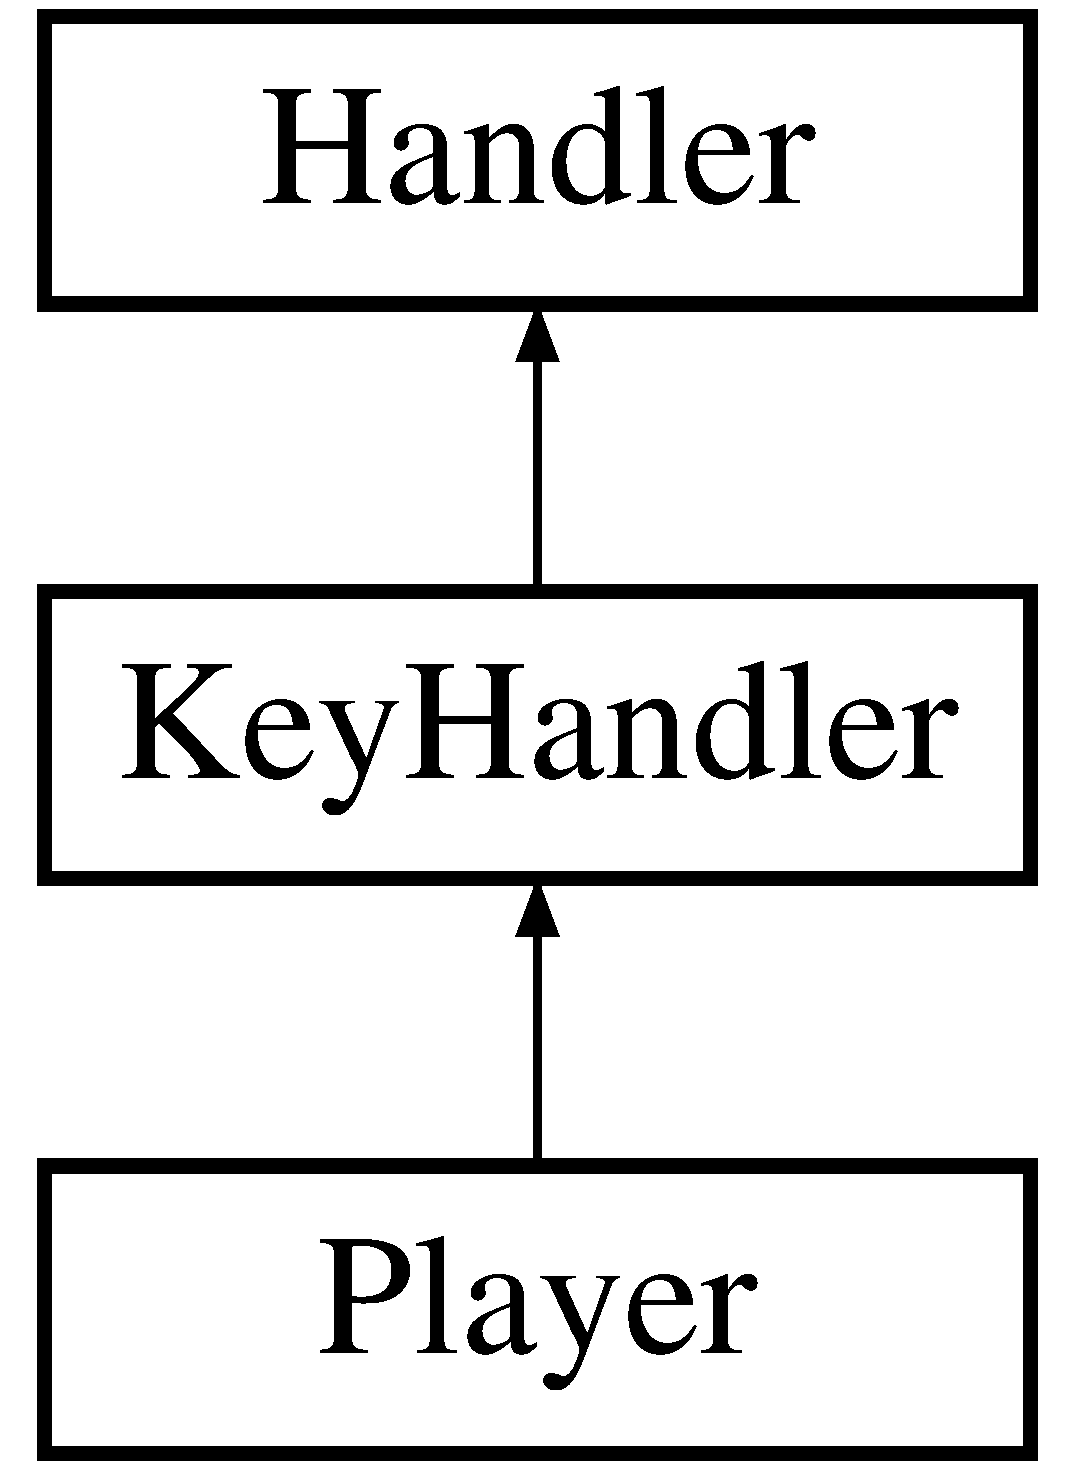
\includegraphics[height=3.000000cm]{class_key_handler}
\end{center}
\end{figure}
\subsection*{Classes}
\begin{DoxyCompactItemize}
\item 
class \hyperlink{class_key_handler_1_1_key}{Key}
\end{DoxyCompactItemize}
\subsection*{Public Member Functions}
\begin{DoxyCompactItemize}
\item 
\hypertarget{class_key_handler_a37dacf5fdd9bb28162562b5b584b49b3}{}\label{class_key_handler_a37dacf5fdd9bb28162562b5b584b49b3} 
{\bfseries Key\+Handler} (class \hyperlink{class_engine}{Engine} $\ast$game)
\item 
\hypertarget{class_key_handler_ab62ed8038ace8783cfb6d2dea1a8821d}{}\label{class_key_handler_ab62ed8038ace8783cfb6d2dea1a8821d} 
virtual void {\bfseries Key\+Up\+Event} (\hyperlink{class_key_handler_1_1_key_a832541e186986ff9f6bd5a810ed5c164}{Key\+::\+Keycode} key\+In, bool alt, bool control, bool shift, bool system)
\item 
\hypertarget{class_key_handler_ac497fa48f5e4fc6e133c110a018f6fb3}{}\label{class_key_handler_ac497fa48f5e4fc6e133c110a018f6fb3} 
virtual void {\bfseries Key\+Dn\+Event} (\hyperlink{class_key_handler_1_1_key_a832541e186986ff9f6bd5a810ed5c164}{Key\+::\+Keycode} key\+In, bool alt, bool control, bool shift, bool system)=0
\end{DoxyCompactItemize}
\subsection*{Additional Inherited Members}


The documentation for this class was generated from the following files\+:\begin{DoxyCompactItemize}
\item 
Handler.\+h\item 
Handler.\+cpp\end{DoxyCompactItemize}

\hypertarget{class_lifebar}{}\section{Lifebar Class Reference}
\label{class_lifebar}\index{Lifebar@{Lifebar}}
Inheritance diagram for Lifebar\+:\begin{figure}[H]
\begin{center}
\leavevmode
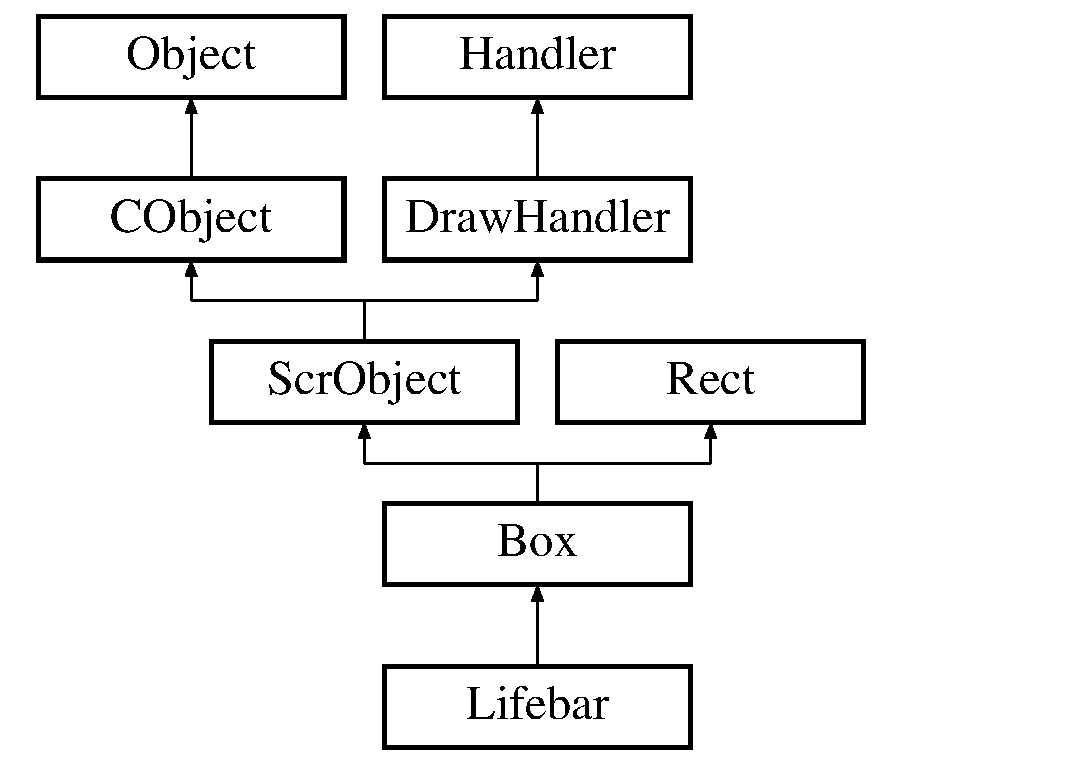
\includegraphics[height=5.000000cm]{class_lifebar}
\end{center}
\end{figure}
\subsection*{Public Member Functions}
\begin{DoxyCompactItemize}
\item 
\hypertarget{class_lifebar_a27922e8a4be8396e1e68ec4ca03b1874}{}\label{class_lifebar_a27922e8a4be8396e1e68ec4ca03b1874} 
{\bfseries Lifebar} (\hyperlink{class_engine}{Engine} $\ast$game, \hyperlink{class_rect}{Rect} refrect)
\item 
\hypertarget{class_lifebar_a0a904e4004820e0d1c0cb5152e69cfbf}{}\label{class_lifebar_a0a904e4004820e0d1c0cb5152e69cfbf} 
void {\bfseries Set\+Health} (double input)
\end{DoxyCompactItemize}
\subsection*{Public Attributes}
\begin{DoxyCompactItemize}
\item 
\hypertarget{class_lifebar_a1fd0dcdaba628c269d0c26301605d2ff}{}\label{class_lifebar_a1fd0dcdaba628c269d0c26301605d2ff} 
\hyperlink{class_square}{Square} {\bfseries squanch}
\end{DoxyCompactItemize}


The documentation for this class was generated from the following file\+:\begin{DoxyCompactItemize}
\item 
Fight\+Game.\+cpp\end{DoxyCompactItemize}

\hypertarget{class_motion}{}\section{Motion Class Reference}
\label{class_motion}\index{Motion@{Motion}}


Helper class that has simple functionality for primitive vector physics calculations.  




{\ttfamily \#include $<$Physics.\+h$>$}

Inheritance diagram for Motion\+:\begin{figure}[H]
\begin{center}
\leavevmode
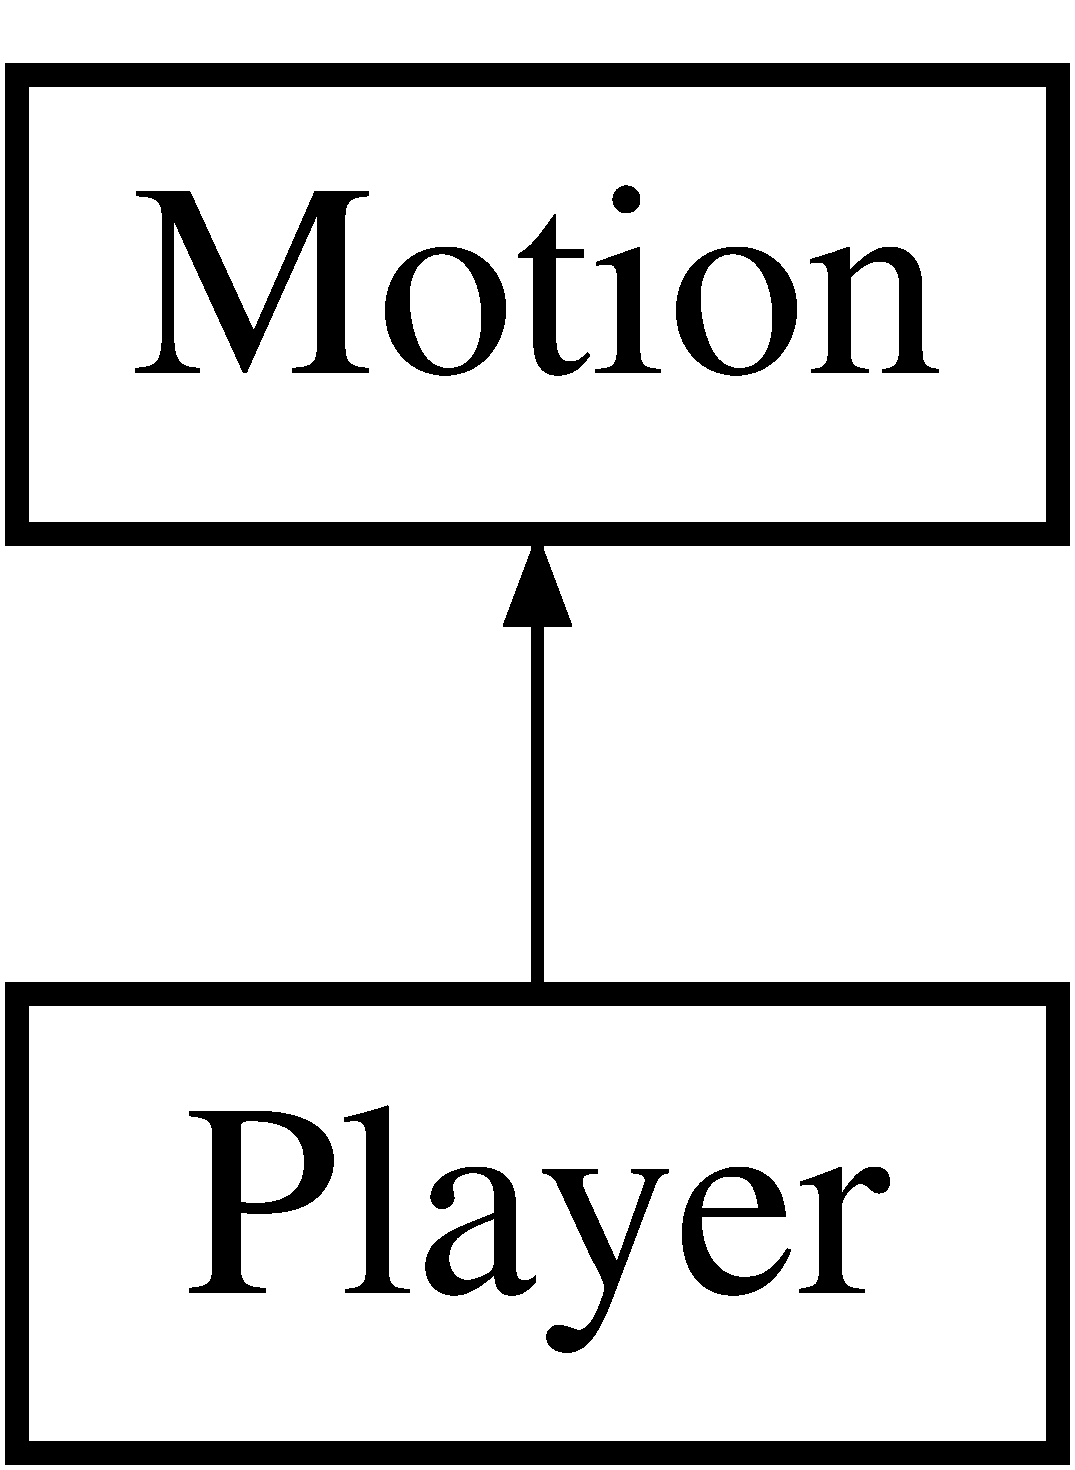
\includegraphics[height=2.000000cm]{class_motion}
\end{center}
\end{figure}
\subsection*{Public Member Functions}
\begin{DoxyCompactItemize}
\item 
\hypertarget{class_motion_a4c7abd6f494d4c6900c41de832b3a81d}{}\label{class_motion_a4c7abd6f494d4c6900c41de832b3a81d} 
\hyperlink{class_motion_a4c7abd6f494d4c6900c41de832b3a81d}{Motion} (double initime, \hyperlink{class_vector2}{Vector2} acc=\hyperlink{class_vector2}{Vector2}(0, 0), \hyperlink{class_vector2}{Vector2} vel=\hyperlink{class_vector2}{Vector2}(0, 0))
\begin{DoxyCompactList}\small\item\em This class must be initialized with starting acceleration and velocity vectors. The time is used during update calculations and should come from the engine\textquotesingle{}s clock. \end{DoxyCompactList}\item 
\hypertarget{class_motion_aa4cda5dcd08b8854ee807e8413a268fc}{}\label{class_motion_aa4cda5dcd08b8854ee807e8413a268fc} 
\hyperlink{class_vector2}{Vector2} \hyperlink{class_motion_aa4cda5dcd08b8854ee807e8413a268fc}{Update} (double rtime)
\begin{DoxyCompactList}\small\item\em This method updates velocity (not acceleration) A\+F\+T\+ER returning the displacement. The time passed in is current engine time. This means that all movement happens a frame later from the last outside update, since the \char`\"{}old\char`\"{} displacement is returned. \end{DoxyCompactList}\item 
\hypertarget{class_motion_af91acfa4e8aba0be029f7a8716f9ee69}{}\label{class_motion_af91acfa4e8aba0be029f7a8716f9ee69} 
\hyperlink{class_vector2}{Vector2} \hyperlink{class_motion_af91acfa4e8aba0be029f7a8716f9ee69}{Get\+Displacement} (double rtime)
\begin{DoxyCompactList}\small\item\em This method returns a displacement based on current velocity. It updates nothing. \end{DoxyCompactList}\end{DoxyCompactItemize}
\subsection*{Public Attributes}
\begin{DoxyCompactItemize}
\item 
\hypertarget{class_motion_a07a9a3095b33bec14859fea515611174}{}\label{class_motion_a07a9a3095b33bec14859fea515611174} 
double {\bfseries l\+Time}
\item 
\hypertarget{class_motion_aee2de6ed8260b8aac72a68b03cf985c3}{}\label{class_motion_aee2de6ed8260b8aac72a68b03cf985c3} 
\hyperlink{class_vector2}{Vector2} {\bfseries acceleration}
\item 
\hypertarget{class_motion_ab1d630ea5dd81de4066665673bd422d6}{}\label{class_motion_ab1d630ea5dd81de4066665673bd422d6} 
\hyperlink{class_vector2}{Vector2} {\bfseries velocity}
\end{DoxyCompactItemize}


\subsection{Detailed Description}
Helper class that has simple functionality for primitive vector physics calculations. 

The documentation for this class was generated from the following files\+:\begin{DoxyCompactItemize}
\item 
Physics.\+h\item 
Physics.\+cpp\end{DoxyCompactItemize}

\hypertarget{class_network_handler}{}\section{Network\+Handler Class Reference}
\label{class_network_handler}\index{Network\+Handler@{Network\+Handler}}
Inheritance diagram for Network\+Handler\+:\begin{figure}[H]
\begin{center}
\leavevmode
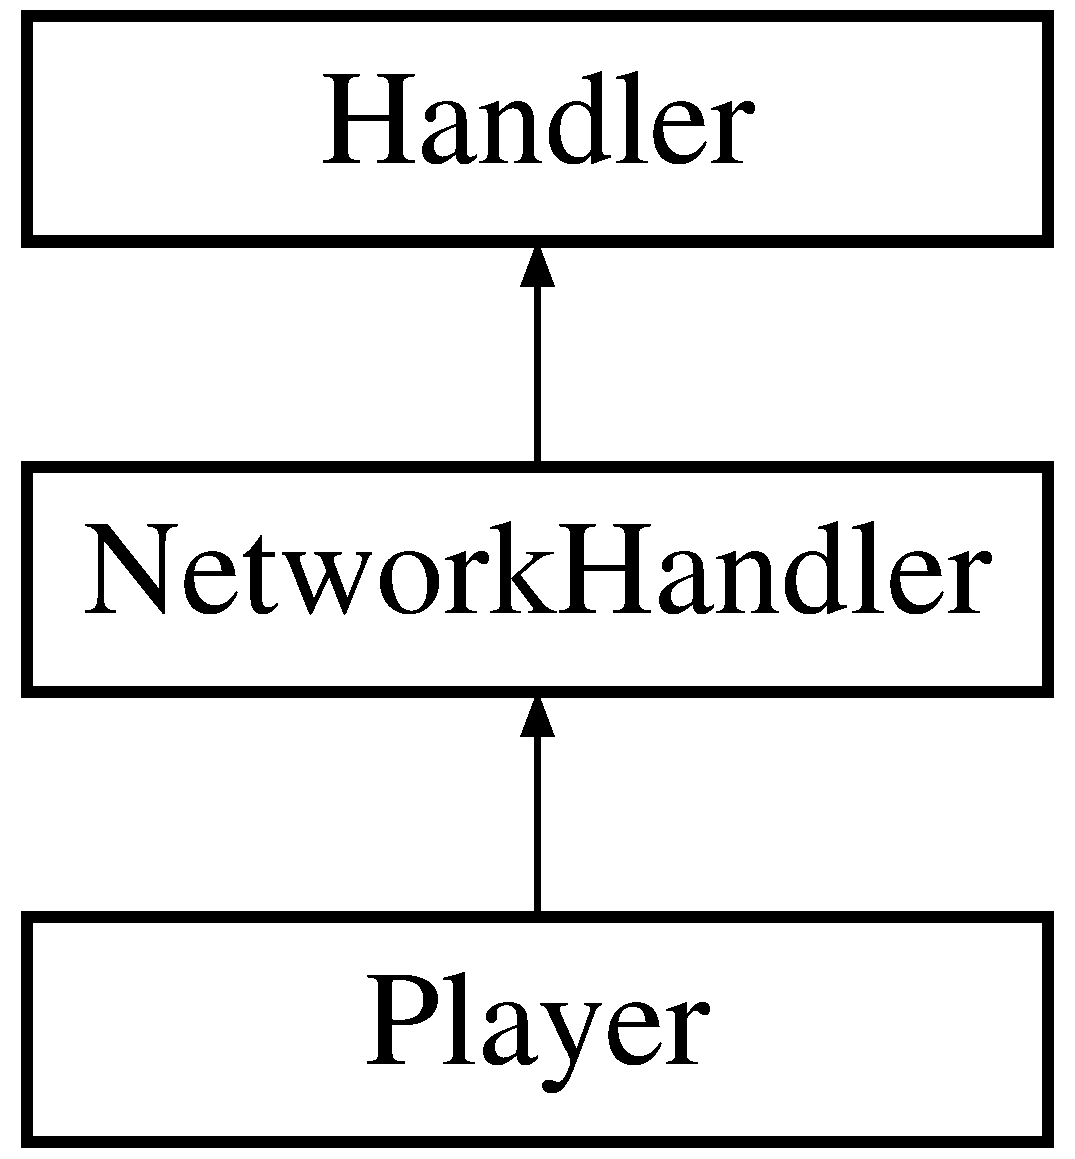
\includegraphics[height=3.000000cm]{class_network_handler}
\end{center}
\end{figure}
\subsection*{Public Member Functions}
\begin{DoxyCompactItemize}
\item 
\hypertarget{class_network_handler_a692fd2010a3dd2bf40cd3aac311b9d53}{}\label{class_network_handler_a692fd2010a3dd2bf40cd3aac311b9d53} 
{\bfseries Network\+Handler} (class \hyperlink{class_engine}{Engine} $\ast$game)
\item 
\hypertarget{class_network_handler_a31dab0982a0da9b6ff4d2a964cd804db}{}\label{class_network_handler_a31dab0982a0da9b6ff4d2a964cd804db} 
virtual void {\bfseries Udp\+Event} (class \hyperlink{class_packet}{Packet} $\ast$pktin, class \hyperlink{class_i_padd}{I\+Padd} addin, unsigned short portin)=0
\end{DoxyCompactItemize}
\subsection*{Additional Inherited Members}


The documentation for this class was generated from the following files\+:\begin{DoxyCompactItemize}
\item 
Handler.\+h\item 
Handler.\+cpp\end{DoxyCompactItemize}

\hypertarget{class_obj_collection}{}\section{Obj\+Collection Class Reference}
\label{class_obj_collection}\index{Obj\+Collection@{Obj\+Collection}}


Container/linked list used to manage Objects.  




{\ttfamily \#include $<$Collection.\+h$>$}

\subsection*{Public Member Functions}
\begin{DoxyCompactItemize}
\item 
\hypertarget{class_obj_collection_ac0edc07cad1b67925b032bd93a9e72d8}{}\label{class_obj_collection_ac0edc07cad1b67925b032bd93a9e72d8} 
\hyperlink{class_obj_collection_ac0edc07cad1b67925b032bd93a9e72d8}{Obj\+Collection} ()
\begin{DoxyCompactList}\small\item\em Inits head to null. \end{DoxyCompactList}\item 
\hypertarget{class_obj_collection_a97764e65b3ced57232008835f938b67a}{}\label{class_obj_collection_a97764e65b3ced57232008835f938b67a} 
\hyperlink{class_obj_collection_a97764e65b3ced57232008835f938b67a}{$\sim$\+Obj\+Collection} ()
\begin{DoxyCompactList}\small\item\em Detaches all objects associated with nodes in this collection, therefore depopulating list as well. \end{DoxyCompactList}\item 
\hypertarget{class_obj_collection_a109344a592e7f2daa0f3b4f5dc9d926d}{}\label{class_obj_collection_a109344a592e7f2daa0f3b4f5dc9d926d} 
void \hyperlink{class_obj_collection_a109344a592e7f2daa0f3b4f5dc9d926d}{Remove} (\hyperlink{struct_obj_ls_node}{Obj\+Ls\+Node} $\ast$target)
\begin{DoxyCompactList}\small\item\em Removes specified node from the list. This is really only called by \hyperlink{class_object}{Object}\textquotesingle{}s Detach(). \end{DoxyCompactList}\item 
\hyperlink{struct_obj_ls_node}{Obj\+Ls\+Node} $\ast$ \hyperlink{class_obj_collection_a0fc6d26772a3f657a41ca9360e65b33f}{Add} (\hyperlink{class_object}{Object} $\ast$input, \hyperlink{class_transform}{Transform} in\+Trans)
\begin{DoxyCompactList}\small\item\em This list adds nodes to the start of the list, not to the end, with the oldest nodes at the end of the list. The pointer returned is used by the \hyperlink{class_object}{Object} associated with this node. \end{DoxyCompactList}\end{DoxyCompactItemize}
\subsection*{Public Attributes}
\begin{DoxyCompactItemize}
\item 
\hypertarget{class_obj_collection_add6095e3454bd7ab4f288ac842cc7fce}{}\label{class_obj_collection_add6095e3454bd7ab4f288ac842cc7fce} 
\hyperlink{struct_obj_ls_node}{Obj\+Ls\+Node} $\ast$ \hyperlink{class_obj_collection_add6095e3454bd7ab4f288ac842cc7fce}{my\+Head}
\begin{DoxyCompactList}\small\item\em The first node in the list. \end{DoxyCompactList}\end{DoxyCompactItemize}


\subsection{Detailed Description}
Container/linked list used to manage Objects. 

Mainly used by C\+Objects. Manages nodes that store pointer information. 

\subsection{Member Function Documentation}
\hypertarget{class_obj_collection_a0fc6d26772a3f657a41ca9360e65b33f}{}\label{class_obj_collection_a0fc6d26772a3f657a41ca9360e65b33f} 
\index{Obj\+Collection@{Obj\+Collection}!Add@{Add}}
\index{Add@{Add}!Obj\+Collection@{Obj\+Collection}}
\subsubsection{\texorpdfstring{Add()}{Add()}}
{\footnotesize\ttfamily \hyperlink{struct_obj_ls_node}{Obj\+Ls\+Node} $\ast$ Obj\+Collection\+::\+Add (\begin{DoxyParamCaption}\item[{\hyperlink{class_object}{Object} $\ast$}]{input,  }\item[{\hyperlink{class_transform}{Transform}}]{in\+Trans }\end{DoxyParamCaption})}



This list adds nodes to the start of the list, not to the end, with the oldest nodes at the end of the list. The pointer returned is used by the \hyperlink{class_object}{Object} associated with this node. 


\begin{DoxyParams}{Parameters}
{\em input} & -\/ The object associated with this node \\
\hline
{\em in\+Trans} & -\/ The transform information to store in the node. Usually this is some offset from the parent\textquotesingle{}s transform. \\
\hline
\end{DoxyParams}


The documentation for this class was generated from the following files\+:\begin{DoxyCompactItemize}
\item 
Collection.\+h\item 
Collection.\+cpp\end{DoxyCompactItemize}

\hypertarget{class_object}{}\section{Object Class Reference}
\label{class_object}\index{Object@{Object}}


Base class for almost all rendered entities in the engine.  




{\ttfamily \#include $<$Object.\+h$>$}

Inheritance diagram for Object\+:\begin{figure}[H]
\begin{center}
\leavevmode
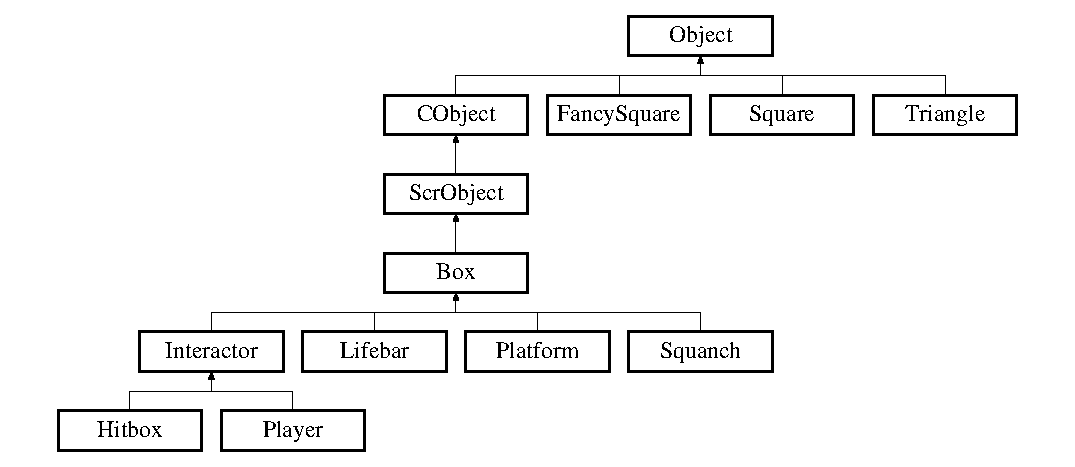
\includegraphics[height=5.833333cm]{class_object}
\end{center}
\end{figure}
\subsection*{Public Member Functions}
\begin{DoxyCompactItemize}
\item 
\hypertarget{class_object_a40860402e64d8008fb42329df7097cdb}{}\label{class_object_a40860402e64d8008fb42329df7097cdb} 
\hyperlink{class_object_a40860402e64d8008fb42329df7097cdb}{Object} ()
\begin{DoxyCompactList}\small\item\em Simple constructor that sets parent and node to null. \end{DoxyCompactList}\item 
\hypertarget{class_object_ae8f5483f459e46687bd01e6f9977afd3}{}\label{class_object_ae8f5483f459e46687bd01e6f9977afd3} 
\hyperlink{class_object_ae8f5483f459e46687bd01e6f9977afd3}{$\sim$\+Object} ()
\begin{DoxyCompactList}\small\item\em The destructor simply calls detach. \end{DoxyCompactList}\item 
virtual void \hyperlink{class_object_adeb7a19aaca51dbf093b37fd21c5e41f}{Draw} (class \hyperlink{class_engine}{Engine} $\ast$game\+Engine, \hyperlink{class_transform}{Transform} parent\+Trans)=0
\begin{DoxyCompactList}\small\item\em Virtual function meant to be implemented by children. Some objects use Draw to pass information, delegating the actual drawing to the objects at the end of the parent-\/child hierarchy. \end{DoxyCompactList}\item 
void \hyperlink{class_object_ab0d9f0a189f0587d672cc21008b2be76}{Attach\+To} (class \hyperlink{class_c_object}{C\+Object} $\ast$target, \hyperlink{class_transform}{Transform} input\+Trans)
\begin{DoxyCompactList}\small\item\em Function to attach objects (whether \hyperlink{class_c_object}{C\+Object} or otherwise) to C\+Objects. This will create a new node and place it in the \hyperlink{class_c_object}{C\+Object}\textquotesingle{}s list, which is appropriately updated. \end{DoxyCompactList}\item 
\hypertarget{class_object_ad818b7d495bf99bedcabfdf0f37774ac}{}\label{class_object_ad818b7d495bf99bedcabfdf0f37774ac} 
void \hyperlink{class_object_ad818b7d495bf99bedcabfdf0f37774ac}{Detach} ()
\begin{DoxyCompactList}\small\item\em Removes this object\textquotesingle{}s node from its parent\textquotesingle{}s collection, then sets its node and parent to null. \end{DoxyCompactList}\item 
\hypertarget{class_object_a9df4b0c95c3af3a00f8193a4a8e5888c}{}\label{class_object_a9df4b0c95c3af3a00f8193a4a8e5888c} 
void \hyperlink{class_object_a9df4b0c95c3af3a00f8193a4a8e5888c}{UpdateT} (\hyperlink{class_transform}{Transform} input)
\begin{DoxyCompactList}\small\item\em Changes the transform information stored in the object\textquotesingle{}s node (if one exists). Note that this overwrites the old transform information if it is not explicitly added to the old one. \end{DoxyCompactList}\end{DoxyCompactItemize}
\subsection*{Public Attributes}
\begin{DoxyCompactItemize}
\item 
\hypertarget{class_object_a986b4a5516d90927038453711be9a4e8}{}\label{class_object_a986b4a5516d90927038453711be9a4e8} 
class \hyperlink{class_c_object}{C\+Object} $\ast$ \hyperlink{class_object_a986b4a5516d90927038453711be9a4e8}{my\+Parent}
\begin{DoxyCompactList}\small\item\em This is the object\textquotesingle{}s parent. Normally, game objects are not drawn if they don\textquotesingle{}t have a parent. \end{DoxyCompactList}\item 
\hypertarget{class_object_ab95df2681777f02917105b7797acde33}{}\label{class_object_ab95df2681777f02917105b7797acde33} 
struct \hyperlink{struct_obj_ls_node}{Obj\+Ls\+Node} $\ast$ \hyperlink{class_object_ab95df2681777f02917105b7797acde33}{my\+Node}
\begin{DoxyCompactList}\small\item\em This points to the node that this object is stored in. This information is used to update the list that the object resides in. It can also be used to change the object\textquotesingle{}s transform. \end{DoxyCompactList}\end{DoxyCompactItemize}


\subsection{Detailed Description}
Base class for almost all rendered entities in the engine. 

Many children inherit from this base class. It provides basic functionality for attaching to C\+Objects and drawing. Since it in always assumed that an \hyperlink{class_object}{Object} has a parent, and since object parents are collections, this makes it easy to make a long hierarchy of game objects. This is particularly useful for passing down transformation info. This also means that rendering occurs according to a parent-\/child hierarchy. 

\subsection{Member Function Documentation}
\hypertarget{class_object_ab0d9f0a189f0587d672cc21008b2be76}{}\label{class_object_ab0d9f0a189f0587d672cc21008b2be76} 
\index{Object@{Object}!Attach\+To@{Attach\+To}}
\index{Attach\+To@{Attach\+To}!Object@{Object}}
\subsubsection{\texorpdfstring{Attach\+To()}{AttachTo()}}
{\footnotesize\ttfamily void Object\+::\+Attach\+To (\begin{DoxyParamCaption}\item[{class \hyperlink{class_c_object}{C\+Object} $\ast$}]{target,  }\item[{\hyperlink{class_transform}{Transform}}]{input\+Trans }\end{DoxyParamCaption})}



Function to attach objects (whether \hyperlink{class_c_object}{C\+Object} or otherwise) to C\+Objects. This will create a new node and place it in the \hyperlink{class_c_object}{C\+Object}\textquotesingle{}s list, which is appropriately updated. 


\begin{DoxyParams}{Parameters}
{\em target} & -\/ Pointer to the \hyperlink{class_c_object}{C\+Object} to be attached to \\
\hline
{\em input\+Trans} & -\/ In Attach\+To, the input transform can be thought of as an offset or difference (using the parent transform as reference). It is stored in the object\textquotesingle{}s node and later added to the parent\textquotesingle{}s transform. \\
\hline
\end{DoxyParams}
\hypertarget{class_object_adeb7a19aaca51dbf093b37fd21c5e41f}{}\label{class_object_adeb7a19aaca51dbf093b37fd21c5e41f} 
\index{Object@{Object}!Draw@{Draw}}
\index{Draw@{Draw}!Object@{Object}}
\subsubsection{\texorpdfstring{Draw()}{Draw()}}
{\footnotesize\ttfamily virtual void Object\+::\+Draw (\begin{DoxyParamCaption}\item[{class \hyperlink{class_engine}{Engine} $\ast$}]{game\+Engine,  }\item[{\hyperlink{class_transform}{Transform}}]{parent\+Trans }\end{DoxyParamCaption})\hspace{0.3cm}{\ttfamily [pure virtual]}}



Virtual function meant to be implemented by children. Some objects use Draw to pass information, delegating the actual drawing to the objects at the end of the parent-\/child hierarchy. 


\begin{DoxyParams}{Parameters}
{\em game\+Engine} & -\/ Pointer to the game engine that will render this \\
\hline
{\em parent\+Trans} & -\/ \hyperlink{class_transform}{Transform} being passed to the object. With long chains of object children/parents, transforms can be cumulative. \\
\hline
\end{DoxyParams}


Implemented in \hyperlink{class_fancy_square_ac77d35ba8ab766f8a3e35f68e7344953}{Fancy\+Square}, \hyperlink{class_c_object_a65338dd4ac20a20340875597344c0c4b}{C\+Object}, \hyperlink{class_square_a9a533e0dd001a0b883bea5145c7444e0}{Square}, and \hyperlink{class_triangle_a2c8418bbe7a955b9ad53571a5832e1b0}{Triangle}.



The documentation for this class was generated from the following files\+:\begin{DoxyCompactItemize}
\item 
Object.\+h\item 
Object.\+cpp\end{DoxyCompactItemize}

\hypertarget{struct_obj_ls_node}{}\section{Obj\+Ls\+Node Struct Reference}
\label{struct_obj_ls_node}\index{Obj\+Ls\+Node@{Obj\+Ls\+Node}}


Basic node used in object lists.  




{\ttfamily \#include $<$Collection.\+h$>$}

\subsection*{Public Member Functions}
\begin{DoxyCompactItemize}
\item 
\hypertarget{struct_obj_ls_node_ab363607829875f39aaaeb69c8e0f73b9}{}\label{struct_obj_ls_node_ab363607829875f39aaaeb69c8e0f73b9} 
\hyperlink{struct_obj_ls_node_ab363607829875f39aaaeb69c8e0f73b9}{Obj\+Ls\+Node} (class \hyperlink{class_object}{Object} $\ast$in\+Obj, class \hyperlink{class_transform}{Transform} in\+Trans)
\begin{DoxyCompactList}\small\item\em Straightforward constructor with init list that simply initializes the supplied arguments. \end{DoxyCompactList}\end{DoxyCompactItemize}
\subsection*{Public Attributes}
\begin{DoxyCompactItemize}
\item 
\hypertarget{struct_obj_ls_node_a2b1d525574c323263c4b6fce4e0a45c4}{}\label{struct_obj_ls_node_a2b1d525574c323263c4b6fce4e0a45c4} 
\hyperlink{class_object}{Object} $\ast$ \hyperlink{struct_obj_ls_node_a2b1d525574c323263c4b6fce4e0a45c4}{my\+Object}
\begin{DoxyCompactList}\small\item\em Pointer to object associated with this node. \end{DoxyCompactList}\item 
\hypertarget{struct_obj_ls_node_aae78b2902eeed5cf1104057251d2bcdc}{}\label{struct_obj_ls_node_aae78b2902eeed5cf1104057251d2bcdc} 
\hyperlink{struct_obj_ls_node}{Obj\+Ls\+Node} $\ast$ \hyperlink{struct_obj_ls_node_aae78b2902eeed5cf1104057251d2bcdc}{next\+Node}
\begin{DoxyCompactList}\small\item\em Pointer to the next node within this node\textquotesingle{}s list. \end{DoxyCompactList}\item 
\hypertarget{struct_obj_ls_node_a99f388a245b879697357c363fd972668}{}\label{struct_obj_ls_node_a99f388a245b879697357c363fd972668} 
\hyperlink{struct_obj_ls_node}{Obj\+Ls\+Node} $\ast$ \hyperlink{struct_obj_ls_node_a99f388a245b879697357c363fd972668}{prev\+Node}
\begin{DoxyCompactList}\small\item\em Pointer to the previous node within this node\textquotesingle{}s list. \end{DoxyCompactList}\item 
\hypertarget{struct_obj_ls_node_aa002f5d20dccf6c1fa442d66538e46b1}{}\label{struct_obj_ls_node_aa002f5d20dccf6c1fa442d66538e46b1} 
\hyperlink{class_transform}{Transform} \hyperlink{struct_obj_ls_node_aa002f5d20dccf6c1fa442d66538e46b1}{my\+Object\+Trans}
\begin{DoxyCompactList}\small\item\em \hyperlink{class_transform}{Transform} information stored when this node is created and/or updated. Usually used to offset an object from its parent transform reference. \end{DoxyCompactList}\end{DoxyCompactItemize}


\subsection{Detailed Description}
Basic node used in object lists. 

Obj\+Ls\+Nodes (\hyperlink{class_object}{Object} list node) populate object collections. They are part of a simple linked list system; they also point to their respective \hyperlink{class_object}{Object} and some supplied \hyperlink{class_transform}{Transform} information. 

The documentation for this struct was generated from the following file\+:\begin{DoxyCompactItemize}
\item 
Collection.\+h\end{DoxyCompactItemize}

\hypertarget{class_packet}{}\section{Packet Class Reference}
\label{class_packet}\index{Packet@{Packet}}


Wrapper for sfml \hyperlink{class_packet}{Packet} class that provides primitive \hyperlink{class_packet}{Packet} generation and manipulation.  




{\ttfamily \#include $<$Network.\+h$>$}

\subsection*{Public Member Functions}
\begin{DoxyCompactItemize}
\item 
\hypertarget{class_packet_a8b4c1dd3fec14925e88df2b0f3fdfa28}{}\label{class_packet_a8b4c1dd3fec14925e88df2b0f3fdfa28} 
\hyperlink{class_packet_a8b4c1dd3fec14925e88df2b0f3fdfa28}{Packet} (sf\+::\+Packet pktin)
\begin{DoxyCompactList}\small\item\em Copy constructor. \end{DoxyCompactList}\item 
\hypertarget{class_packet_ad9268e17dd1ec9c3ed5ba8630dd6a5d0}{}\label{class_packet_ad9268e17dd1ec9c3ed5ba8630dd6a5d0} 
void {\bfseries Stuff\+Me} (double input)
\item 
\hypertarget{class_packet_a16415c06803e885529f1f7fba7455dc3}{}\label{class_packet_a16415c06803e885529f1f7fba7455dc3} 
void {\bfseries Stuff\+Me} (int input)
\item 
\hypertarget{class_packet_a0828dded7d7aae907bff02a897e2d0b8}{}\label{class_packet_a0828dded7d7aae907bff02a897e2d0b8} 
void {\bfseries Stuff\+Me} (bool input)
\item 
\hypertarget{class_packet_af9dd66e7668001601b01e024b3909c26}{}\label{class_packet_af9dd66e7668001601b01e024b3909c26} 
void {\bfseries Pop\+Me} (double $\ast$input)
\item 
\hypertarget{class_packet_a870a5bc6e8efb188459d474360a7b6bd}{}\label{class_packet_a870a5bc6e8efb188459d474360a7b6bd} 
void {\bfseries Pop\+Me} (int $\ast$input)
\item 
\hypertarget{class_packet_a48e1b1bbb9a3a31f730136a13c4c7f73}{}\label{class_packet_a48e1b1bbb9a3a31f730136a13c4c7f73} 
void {\bfseries Pop\+Me} (bool $\ast$input)
\end{DoxyCompactItemize}
\subsection*{Public Attributes}
\begin{DoxyCompactItemize}
\item 
\hypertarget{class_packet_acd7d675f2640238e3926d4489cf26e30}{}\label{class_packet_acd7d675f2640238e3926d4489cf26e30} 
sf\+::\+Packet {\bfseries belly}
\end{DoxyCompactItemize}


\subsection{Detailed Description}
Wrapper for sfml \hyperlink{class_packet}{Packet} class that provides primitive \hyperlink{class_packet}{Packet} generation and manipulation. 

Stuff\+Me methods place data of the appropriate type into the packet. They can be placed into outside variables using pointers together with Pop\+Me methods. Variables must be popped out in the same order they were stuffed in. 

The documentation for this class was generated from the following files\+:\begin{DoxyCompactItemize}
\item 
Network.\+h\item 
Network.\+cpp\end{DoxyCompactItemize}

\hypertarget{class_platform}{}\section{Platform Class Reference}
\label{class_platform}\index{Platform@{Platform}}
Inheritance diagram for Platform\+:\begin{figure}[H]
\begin{center}
\leavevmode
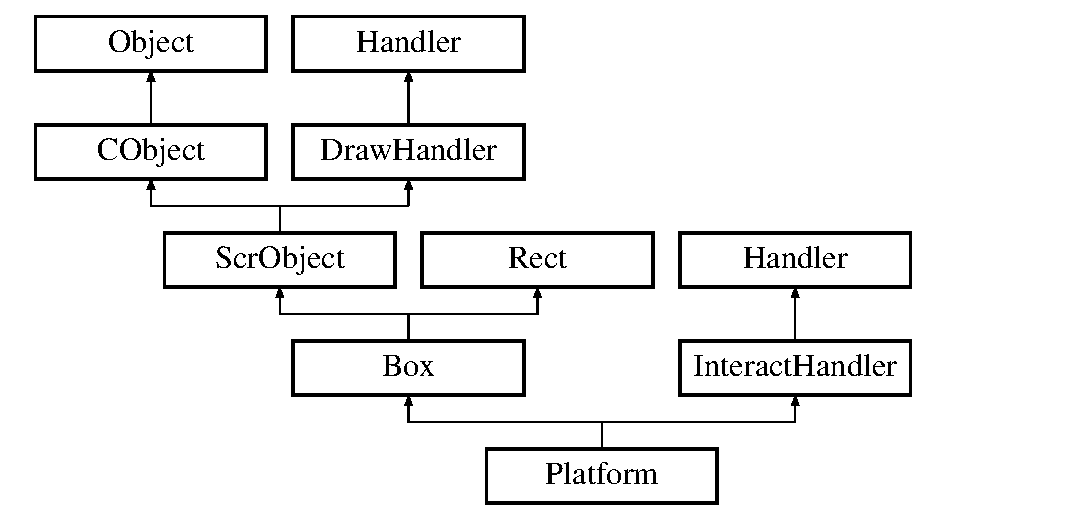
\includegraphics[height=5.000000cm]{class_platform}
\end{center}
\end{figure}
\subsection*{Public Member Functions}
\begin{DoxyCompactItemize}
\item 
\hypertarget{class_platform_aed64a657550c688d2b8a3087cf85d345}{}\label{class_platform_aed64a657550c688d2b8a3087cf85d345} 
{\bfseries Platform} (\hyperlink{class_engine}{Engine} $\ast$game, \hyperlink{class_rect}{Rect} refrect)
\item 
\hypertarget{class_platform_a18a98565e486b1113f729cf737178069}{}\label{class_platform_a18a98565e486b1113f729cf737178069} 
void {\bfseries Interact\+Event} (class \hyperlink{class_scr_object}{Scr\+Object} $\ast$obj)
\end{DoxyCompactItemize}
\subsection*{Public Attributes}
\begin{DoxyCompactItemize}
\item 
\hypertarget{class_platform_ae0c7c9a6a9a6eaa040d35eb245d7bd37}{}\label{class_platform_ae0c7c9a6a9a6eaa040d35eb245d7bd37} 
\hyperlink{class_square}{Square} {\bfseries squanch}
\end{DoxyCompactItemize}


The documentation for this class was generated from the following file\+:\begin{DoxyCompactItemize}
\item 
Fight\+Game.\+cpp\end{DoxyCompactItemize}

\hypertarget{class_player}{}\section{Player Class Reference}
\label{class_player}\index{Player@{Player}}
Inheritance diagram for Player\+:\begin{figure}[H]
\begin{center}
\leavevmode
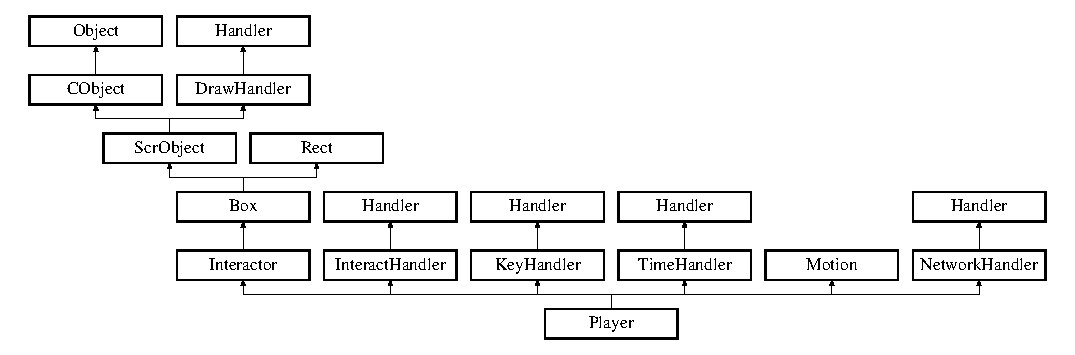
\includegraphics[height=4.324325cm]{class_player}
\end{center}
\end{figure}
\subsection*{Public Member Functions}
\begin{DoxyCompactItemize}
\item 
\hypertarget{class_player_ae06a51f500b10368dd5ebb7853566b22}{}\label{class_player_ae06a51f500b10368dd5ebb7853566b22} 
{\bfseries Player} (\hyperlink{class_engine}{Engine} $\ast$game, \hyperlink{class_rect}{Rect} refrect, const char $\ast$input, const char $\ast$input2, int ID)
\item 
\hypertarget{class_player_afb17544a1c1d12cba93e77a25fbd27a9}{}\label{class_player_afb17544a1c1d12cba93e77a25fbd27a9} 
void {\bfseries Sprite\+Proc} ()
\item 
\hypertarget{class_player_a79060b32a95ca6e3f7a482b9ed45fa07}{}\label{class_player_a79060b32a95ca6e3f7a482b9ed45fa07} 
void {\bfseries Take\+Damage} ()
\item 
\hypertarget{class_player_aa6077bbdf83a68e49deec5425fa490a5}{}\label{class_player_aa6077bbdf83a68e49deec5425fa490a5} 
void {\bfseries Interact\+Event} (class \hyperlink{class_scr_object}{Scr\+Object} $\ast$obj)
\item 
\hypertarget{class_player_acb2790a9c737e1b9c1ab744abdcbc6a0}{}\label{class_player_acb2790a9c737e1b9c1ab744abdcbc6a0} 
void {\bfseries Interact\+Player} (class \hyperlink{class_player}{Player} $\ast$other)
\item 
\hypertarget{class_player_a89d63167bff6dac4cb9a04265908457b}{}\label{class_player_a89d63167bff6dac4cb9a04265908457b} 
void {\bfseries Interact\+Platform} (class \hyperlink{class_platform}{Platform} $\ast$other)
\item 
\hypertarget{class_player_a1334990b8b7aaaad904e22f03f4d947d}{}\label{class_player_a1334990b8b7aaaad904e22f03f4d947d} 
void {\bfseries Jump} ()
\item 
\hypertarget{class_player_a6c879db24d39d894207e078eb4c56e8d}{}\label{class_player_a6c879db24d39d894207e078eb4c56e8d} 
void {\bfseries Attack} ()
\item 
\hypertarget{class_player_ac9d22befc482bf7f2ae7956d9116baf6}{}\label{class_player_ac9d22befc482bf7f2ae7956d9116baf6} 
void {\bfseries Key\+Dn\+Event} (\hyperlink{class_key_handler_1_1_key_a832541e186986ff9f6bd5a810ed5c164}{Key\+::\+Keycode} key\+In, bool alt, bool control, bool shift, bool system)
\item 
\hypertarget{class_player_ae849a9d15bb49f8be75b792eb0ad91ff}{}\label{class_player_ae849a9d15bb49f8be75b792eb0ad91ff} 
void {\bfseries Time\+Event} (double curr\+Time)
\item 
\hypertarget{class_player_a5f4e16ffd07d713353123f5778f1d9b6}{}\label{class_player_a5f4e16ffd07d713353123f5778f1d9b6} 
void {\bfseries Key\+Up\+Event} (\hyperlink{class_key_handler_1_1_key_a832541e186986ff9f6bd5a810ed5c164}{Key\+::\+Keycode} key\+In, bool alt, bool control, bool shift, bool system)
\item 
\hypertarget{class_player_a5feaecbb7796f319449f2fd7abd7c226}{}\label{class_player_a5feaecbb7796f319449f2fd7abd7c226} 
void {\bfseries Udp\+Event} (class \hyperlink{class_packet}{Packet} $\ast$pktin, class \hyperlink{class_i_padd}{I\+Padd} addin, unsigned short portin)
\end{DoxyCompactItemize}
\subsection*{Public Attributes}
\begin{DoxyCompactItemize}
\item 
\hypertarget{class_player_af56d931c400cdea7c22e8160093037e3}{}\label{class_player_af56d931c400cdea7c22e8160093037e3} 
\hyperlink{class_fancy_square}{Fancy\+Square} {\bfseries idle\+Spr}
\item 
\hypertarget{class_player_a2541c4c6dc509de5a68752d4e9d43d15}{}\label{class_player_a2541c4c6dc509de5a68752d4e9d43d15} 
\hyperlink{class_fancy_square}{Fancy\+Square} {\bfseries atk\+Spr}
\item 
\hypertarget{class_player_a4c90c45b5567f3ad77ab62b836a4538d}{}\label{class_player_a4c90c45b5567f3ad77ab62b836a4538d} 
\hyperlink{class_lifebar}{Lifebar} {\bfseries guts}
\item 
\hypertarget{class_player_a33c1b79f3bd3885c420d88acee0431f7}{}\label{class_player_a33c1b79f3bd3885c420d88acee0431f7} 
int {\bfseries player\+ID}
\item 
\hypertarget{class_player_aad3727f9bbaeaffc4ba09c7805ad2a09}{}\label{class_player_aad3727f9bbaeaffc4ba09c7805ad2a09} 
bool {\bfseries in\+Air}
\item 
\hypertarget{class_player_a319ddbd239b2114102f0d6e742c6f8b0}{}\label{class_player_a319ddbd239b2114102f0d6e742c6f8b0} 
bool {\bfseries facing\+Right}
\item 
\hypertarget{class_player_a332b68cd95ad6ef4b513f8bfdd416951}{}\label{class_player_a332b68cd95ad6ef4b513f8bfdd416951} 
bool {\bfseries in\+Atk}
\item 
\hypertarget{class_player_a9a1e8db696e64fae86431fd60076c2ea}{}\label{class_player_a9a1e8db696e64fae86431fd60076c2ea} 
double {\bfseries atk\+Timer}
\item 
\hypertarget{class_player_a60d5cfe903e32557ff4847d1409f7cd1}{}\label{class_player_a60d5cfe903e32557ff4847d1409f7cd1} 
double {\bfseries atk\+CD}
\item 
\hypertarget{class_player_a3b5a5fceb2d734ca5816bf509e78ca9d}{}\label{class_player_a3b5a5fceb2d734ca5816bf509e78ca9d} 
double {\bfseries invul\+Timer}
\item 
\hypertarget{class_player_ab2b72a8e3b80192e49d77c79ffdd2d01}{}\label{class_player_ab2b72a8e3b80192e49d77c79ffdd2d01} 
double {\bfseries invul\+CD}
\item 
\hypertarget{class_player_a231c9aa13c1530858d5b16069935a725}{}\label{class_player_a231c9aa13c1530858d5b16069935a725} 
double {\bfseries atk\+Width}
\item 
\hypertarget{class_player_a8787ba98f514093218da0b971c7db8b3}{}\label{class_player_a8787ba98f514093218da0b971c7db8b3} 
double {\bfseries atk\+Height}
\item 
\hypertarget{class_player_a359f983f7b2e401f4d9f35ad24a082b8}{}\label{class_player_a359f983f7b2e401f4d9f35ad24a082b8} 
double {\bfseries y\+Adjust}
\item 
\hypertarget{class_player_aa5b271dcb0c0843a5f5694565bcad3a0}{}\label{class_player_aa5b271dcb0c0843a5f5694565bcad3a0} 
double {\bfseries health}
\end{DoxyCompactItemize}


The documentation for this class was generated from the following file\+:\begin{DoxyCompactItemize}
\item 
Fight\+Game.\+cpp\end{DoxyCompactItemize}

\hypertarget{class_rect}{}\section{Rect Class Reference}
\label{class_rect}\index{Rect@{Rect}}


Class used for making boxes used in collisions and Screen Objects.  




{\ttfamily \#include $<$Vector.\+h$>$}

Inheritance diagram for Rect\+:\begin{figure}[H]
\begin{center}
\leavevmode
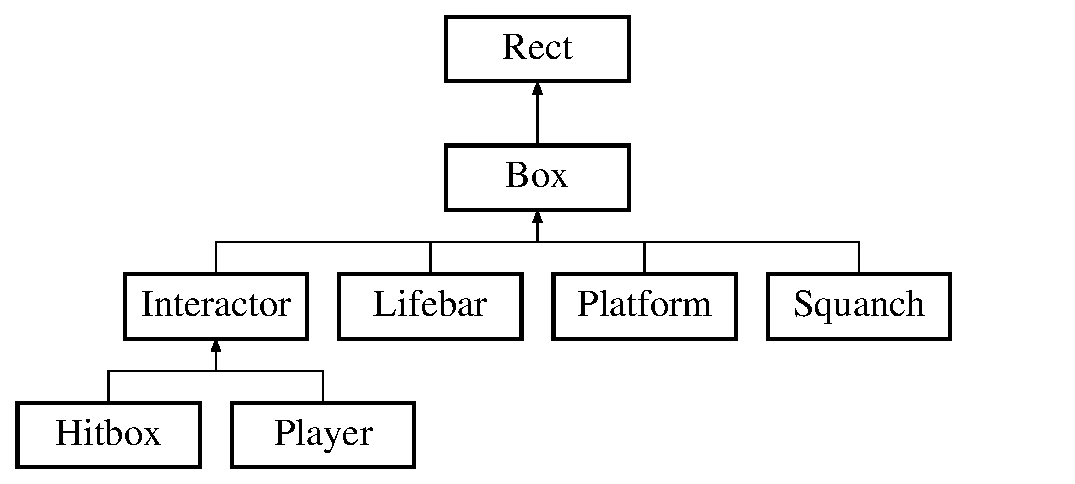
\includegraphics[height=4.000000cm]{class_rect}
\end{center}
\end{figure}
\subsection*{Public Member Functions}
\begin{DoxyCompactItemize}
\item 
\hyperlink{class_rect_ad24b6cae9dd49da138e054b7b7b5ac3f}{Rect} (\hyperlink{class_vector2}{Vector2} p1, \hyperlink{class_vector2}{Vector2} p2)
\begin{DoxyCompactList}\small\item\em Constructor that accepts two points. \end{DoxyCompactList}\item 
\hypertarget{class_rect_a3f92c92e465b3a789f4da3e0d295c53a}{}\label{class_rect_a3f92c92e465b3a789f4da3e0d295c53a} 
\hyperlink{class_rect_a3f92c92e465b3a789f4da3e0d295c53a}{Rect} (const \hyperlink{class_rect}{Rect} \&thing)
\begin{DoxyCompactList}\small\item\em Copy constructor. \end{DoxyCompactList}\item 
\hypertarget{class_rect_a176d3cbbec5903c85063cac2fb380afc}{}\label{class_rect_a176d3cbbec5903c85063cac2fb380afc} 
\hyperlink{class_rect}{Rect} {\bfseries operator+} (const \hyperlink{class_vector2}{Vector2} \&vecin)
\item 
\hypertarget{class_rect_a9aeefc780b44fc2cf9c151e4c24cba9d}{}\label{class_rect_a9aeefc780b44fc2cf9c151e4c24cba9d} 
\hyperlink{class_rect}{Rect} \& {\bfseries operator=} (const \hyperlink{class_rect}{Rect} \&thing)
\item 
\hypertarget{class_rect_abe5622a1eb8736a2022e3e01ea983c73}{}\label{class_rect_abe5622a1eb8736a2022e3e01ea983c73} 
\hyperlink{class_vector2}{Vector2} {\bfseries Get\+Center} ()
\item 
\hypertarget{class_rect_a5744f2db0f140913670eeda0649ab201}{}\label{class_rect_a5744f2db0f140913670eeda0649ab201} 
bool \hyperlink{class_rect_a5744f2db0f140913670eeda0649ab201}{Check\+Overlap} (\hyperlink{class_rect}{Rect} other\+Box)
\begin{DoxyCompactList}\small\item\em Checks if an overlap occurs with the argument. \end{DoxyCompactList}\item 
\hypertarget{class_rect_ae4e3467a3e1f5c23686326a8c6bbafcf}{}\label{class_rect_ae4e3467a3e1f5c23686326a8c6bbafcf} 
double {\bfseries Get\+Height} ()
\item 
\hypertarget{class_rect_a193f7f6cfb2a58c7b66e1143d1ddeb10}{}\label{class_rect_a193f7f6cfb2a58c7b66e1143d1ddeb10} 
double {\bfseries Get\+Width} ()
\item 
\hypertarget{class_rect_a098ae9f097da18fb509f873305d066ed}{}\label{class_rect_a098ae9f097da18fb509f873305d066ed} 
void \hyperlink{class_rect_a098ae9f097da18fb509f873305d066ed}{Displace} (\hyperlink{class_vector2}{Vector2} inputvec)
\begin{DoxyCompactList}\small\item\em Displaces the rect by the supplied vector. \end{DoxyCompactList}\item 
\hypertarget{class_rect_a8d32f2a6333f11f6c415823dd352f631}{}\label{class_rect_a8d32f2a6333f11f6c415823dd352f631} 
void \hyperlink{class_rect_a8d32f2a6333f11f6c415823dd352f631}{Place} (\hyperlink{class_vector2}{Vector2} inputvec)
\begin{DoxyCompactList}\small\item\em Places the rect (centered) at the supplied point. \end{DoxyCompactList}\end{DoxyCompactItemize}
\subsection*{Public Attributes}
\begin{DoxyCompactItemize}
\item 
\hypertarget{class_rect_a6ce67f181f04d552c5b618e47b282a80}{}\label{class_rect_a6ce67f181f04d552c5b618e47b282a80} 
\hyperlink{class_vector2}{Vector2} {\bfseries pt1}
\item 
\hypertarget{class_rect_a691c7827e063156b2cefbb1f2d74b6f5}{}\label{class_rect_a691c7827e063156b2cefbb1f2d74b6f5} 
\hyperlink{class_vector2}{Vector2} {\bfseries pt2}
\end{DoxyCompactItemize}


\subsection{Detailed Description}
Class used for making boxes used in collisions and Screen Objects. 

This class is mainly used as a reference space for Screen Objects. It defines a box with many useful methods good for checking collisions and moving the box around. 

\subsection{Constructor \& Destructor Documentation}
\hypertarget{class_rect_ad24b6cae9dd49da138e054b7b7b5ac3f}{}\label{class_rect_ad24b6cae9dd49da138e054b7b7b5ac3f} 
\index{Rect@{Rect}!Rect@{Rect}}
\index{Rect@{Rect}!Rect@{Rect}}
\subsubsection{\texorpdfstring{Rect()}{Rect()}}
{\footnotesize\ttfamily Rect\+::\+Rect (\begin{DoxyParamCaption}\item[{\hyperlink{class_vector2}{Vector2}}]{p1,  }\item[{\hyperlink{class_vector2}{Vector2}}]{p2 }\end{DoxyParamCaption})}



Constructor that accepts two points. 


\begin{DoxyParams}{Parameters}
{\em p1} & -\/ The first point must always be the lower left point of the rect. \\
\hline
{\em p2} & -\/ The second point must always be the top right point of the rect. \\
\hline
\end{DoxyParams}


The documentation for this class was generated from the following files\+:\begin{DoxyCompactItemize}
\item 
Vector.\+h\item 
Vector.\+cpp\end{DoxyCompactItemize}

\hypertarget{class_rotate}{}\section{Rotate Class Reference}
\label{class_rotate}\index{Rotate@{Rotate}}
Inheritance diagram for Rotate\+:\begin{figure}[H]
\begin{center}
\leavevmode
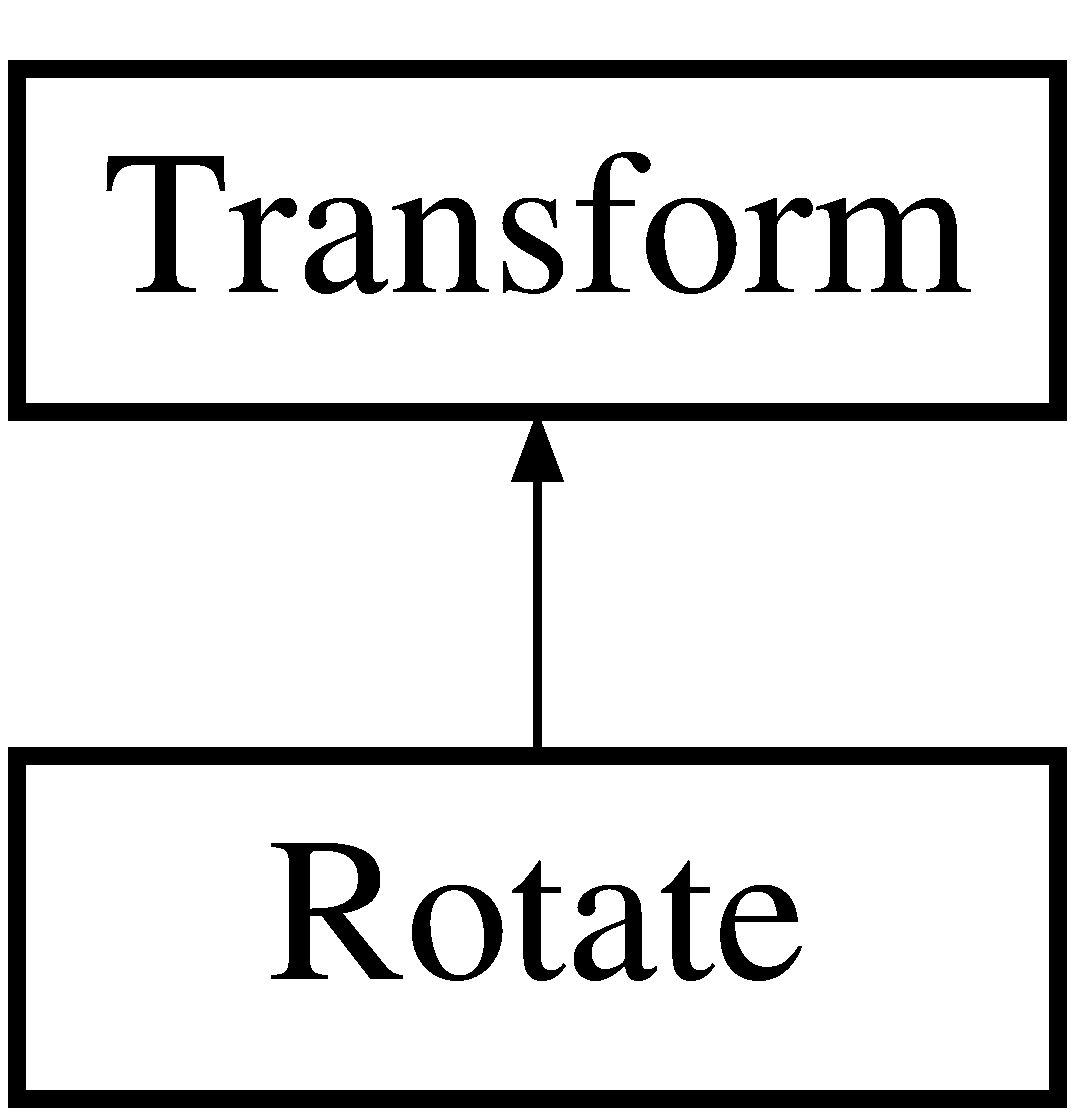
\includegraphics[height=2.000000cm]{class_rotate}
\end{center}
\end{figure}
\subsection*{Public Member Functions}
\begin{DoxyCompactItemize}
\item 
\hypertarget{class_rotate_a9e117ee1fdce26779ee0fb4605d4e8ac}{}\label{class_rotate_a9e117ee1fdce26779ee0fb4605d4e8ac} 
{\bfseries Rotate} (double angle)
\end{DoxyCompactItemize}
\subsection*{Additional Inherited Members}


The documentation for this class was generated from the following file\+:\begin{DoxyCompactItemize}
\item 
Transform.\+h\end{DoxyCompactItemize}

\hypertarget{class_scale}{}\section{Scale Class Reference}
\label{class_scale}\index{Scale@{Scale}}
Inheritance diagram for Scale\+:\begin{figure}[H]
\begin{center}
\leavevmode
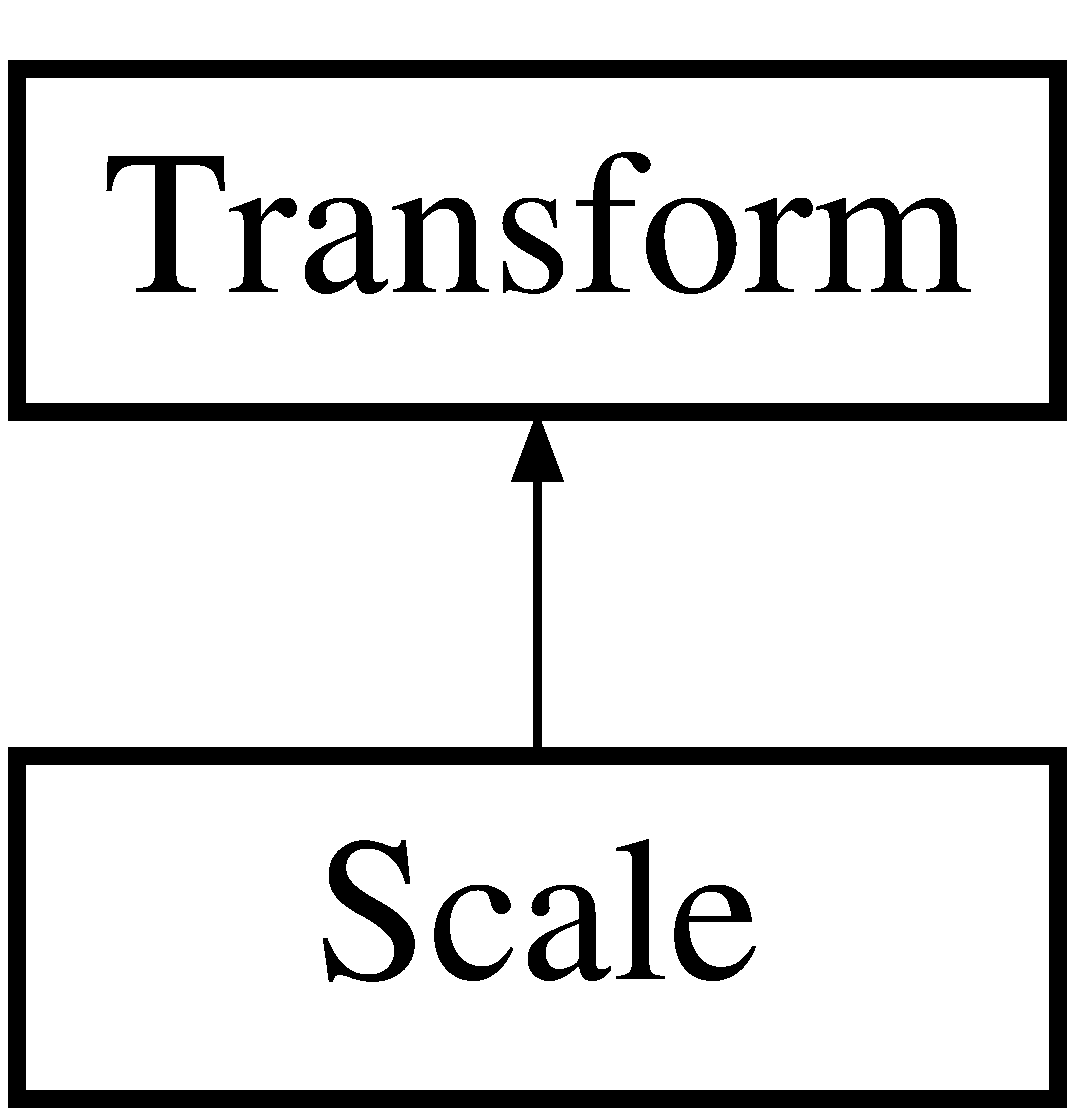
\includegraphics[height=2.000000cm]{class_scale}
\end{center}
\end{figure}
\subsection*{Public Member Functions}
\begin{DoxyCompactItemize}
\item 
\hypertarget{class_scale_a764037517d6d322c62ecaa239e8118f3}{}\label{class_scale_a764037517d6d322c62ecaa239e8118f3} 
{\bfseries Scale} (\hyperlink{class_vector}{Vector} input)
\item 
\hypertarget{class_scale_ab6dce279bf01982adf281ca67bd4ca93}{}\label{class_scale_ab6dce279bf01982adf281ca67bd4ca93} 
{\bfseries Scale} (double x, double y, double z)
\item 
\hypertarget{class_scale_aec810bcc0db8deb0a1ab4b62004c63d3}{}\label{class_scale_aec810bcc0db8deb0a1ab4b62004c63d3} 
{\bfseries Scale} (double input)
\end{DoxyCompactItemize}
\subsection*{Additional Inherited Members}


The documentation for this class was generated from the following file\+:\begin{DoxyCompactItemize}
\item 
Transform.\+h\end{DoxyCompactItemize}

\hypertarget{class_scr_object}{}\section{Scr\+Object Class Reference}
\label{class_scr_object}\index{Scr\+Object@{Scr\+Object}}


Short for Screen\+Object, this is a useful base class with a transformation hierarchy and draw functionality.  




{\ttfamily \#include $<$Scr\+Obj.\+h$>$}

Inheritance diagram for Scr\+Object\+:\begin{figure}[H]
\begin{center}
\leavevmode
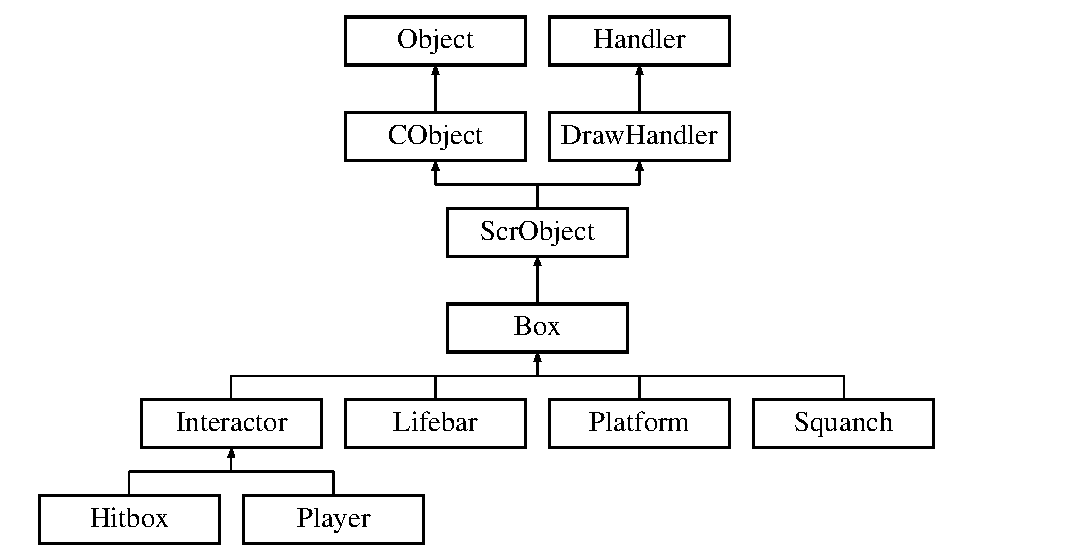
\includegraphics[height=6.000000cm]{class_scr_object}
\end{center}
\end{figure}
\subsection*{Public Member Functions}
\begin{DoxyCompactItemize}
\item 
\hypertarget{class_scr_object_a18bb8e44e47711db6e13482d810ad83d}{}\label{class_scr_object_a18bb8e44e47711db6e13482d810ad83d} 
{\bfseries Scr\+Object} (class \hyperlink{class_engine}{Engine} $\ast$game)
\end{DoxyCompactItemize}
\subsection*{Additional Inherited Members}


\subsection{Detailed Description}
Short for Screen\+Object, this is a useful base class with a transformation hierarchy and draw functionality. 

This class is mainly derived from to make other useful bases. \hyperlink{class_c_object}{C\+Object} provides a transformation hierarchy and object collection, while \hyperlink{class_draw_handler}{Draw\+Handler} provides rendering functionality. 

The documentation for this class was generated from the following files\+:\begin{DoxyCompactItemize}
\item 
Scr\+Obj.\+h\item 
Scr\+Obj.\+cpp\end{DoxyCompactItemize}

\hypertarget{class_shade}{}\section{Shade Class Reference}
\label{class_shade}\index{Shade@{Shade}}
Inheritance diagram for Shade\+:\begin{figure}[H]
\begin{center}
\leavevmode
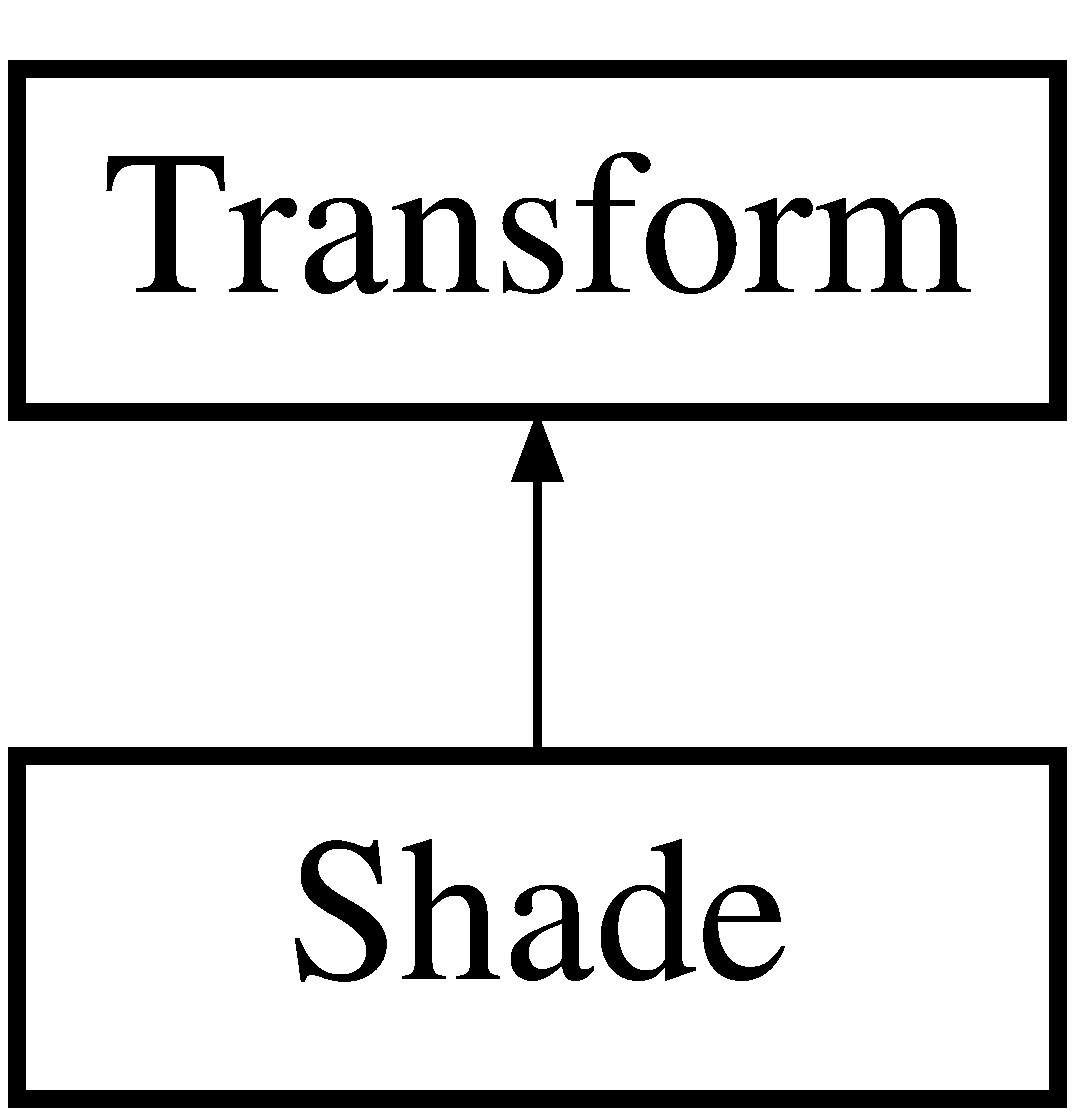
\includegraphics[height=2.000000cm]{class_shade}
\end{center}
\end{figure}
\subsection*{Public Member Functions}
\begin{DoxyCompactItemize}
\item 
\hypertarget{class_shade_afdd84308cff9eebdd2d929079c64bb37}{}\label{class_shade_afdd84308cff9eebdd2d929079c64bb37} 
{\bfseries Shade} (\hyperlink{class_color}{Color} input)
\item 
\hypertarget{class_shade_a6602fccca82ffc97289403f1183bf18e}{}\label{class_shade_a6602fccca82ffc97289403f1183bf18e} 
{\bfseries Shade} (double R, double G, double B)
\item 
\hypertarget{class_shade_ac6c7c2a972788bbbad1504a39690dcde}{}\label{class_shade_ac6c7c2a972788bbbad1504a39690dcde} 
{\bfseries Shade} (double input)
\end{DoxyCompactItemize}
\subsection*{Additional Inherited Members}


The documentation for this class was generated from the following file\+:\begin{DoxyCompactItemize}
\item 
Transform.\+h\end{DoxyCompactItemize}

\hypertarget{class_shift}{}\section{Shift Class Reference}
\label{class_shift}\index{Shift@{Shift}}
Inheritance diagram for Shift\+:\begin{figure}[H]
\begin{center}
\leavevmode
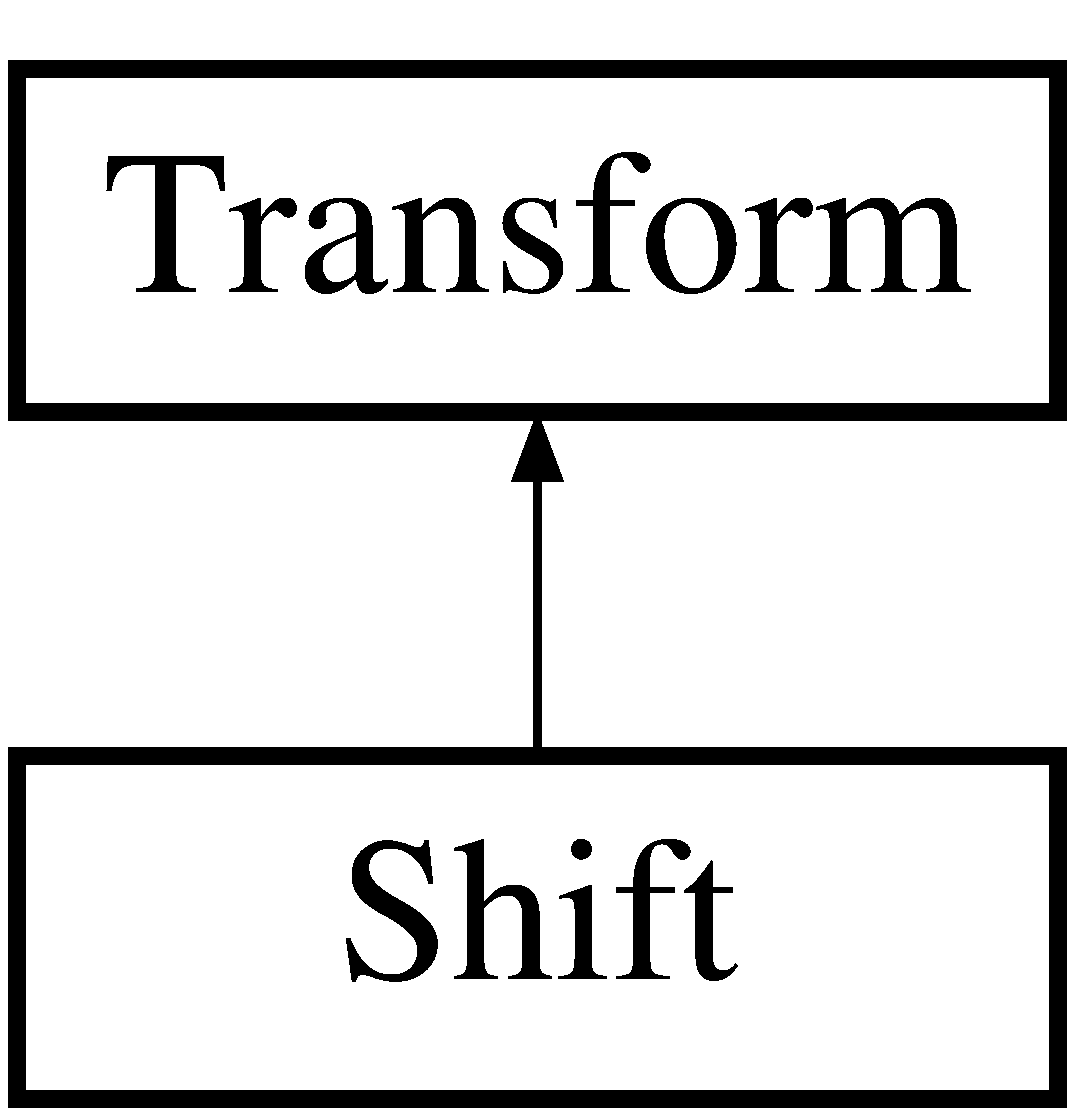
\includegraphics[height=2.000000cm]{class_shift}
\end{center}
\end{figure}
\subsection*{Public Member Functions}
\begin{DoxyCompactItemize}
\item 
\hypertarget{class_shift_a578c0679c998e3a34b9e3ae529e78ab4}{}\label{class_shift_a578c0679c998e3a34b9e3ae529e78ab4} 
{\bfseries Shift} (\hyperlink{class_vector}{Vector} input)
\item 
\hypertarget{class_shift_aabc77a031682d7ae89d5e113edd28770}{}\label{class_shift_aabc77a031682d7ae89d5e113edd28770} 
{\bfseries Shift} (double x, double y, double z)
\end{DoxyCompactItemize}
\subsection*{Additional Inherited Members}


The documentation for this class was generated from the following file\+:\begin{DoxyCompactItemize}
\item 
Transform.\+h\end{DoxyCompactItemize}

\hypertarget{class_split_model}{}\section{Split\+Model Class Reference}
\label{class_split_model}\index{Split\+Model@{Split\+Model}}
\subsection*{Public Member Functions}
\begin{DoxyCompactItemize}
\item 
\hypertarget{class_split_model_a2a29d100a2858da27db5f73236753a5a}{}\label{class_split_model_a2a29d100a2858da27db5f73236753a5a} 
{\bfseries Split\+Model} (G\+Lfloat points\mbox{[}$\,$\mbox{]}, int size)
\item 
\hypertarget{class_split_model_a08efefbd04dcfaebc4de31ea0380b844}{}\label{class_split_model_a08efefbd04dcfaebc4de31ea0380b844} 
void {\bfseries init} (G\+Lfloat points\mbox{[}$\,$\mbox{]}, int size)
\item 
\hypertarget{class_split_model_a45ba9a4c0ddd51542e34f8a47b3a2357}{}\label{class_split_model_a45ba9a4c0ddd51542e34f8a47b3a2357} 
glm\+::vec3 $\ast$ {\bfseries get\+Translation\+Ptr} ()
\item 
\hypertarget{class_split_model_aeac718718504e7b7c096e6654e30b6ae}{}\label{class_split_model_aeac718718504e7b7c096e6654e30b6ae} 
glm\+::vec3 $\ast$ {\bfseries get\+Rotation\+Ptr} ()
\item 
\hypertarget{class_split_model_a25cb815e58bb751d7d2b5b776a2c26ad}{}\label{class_split_model_a25cb815e58bb751d7d2b5b776a2c26ad} 
glm\+::vec3 $\ast$ {\bfseries get\+Scale\+Ptr} ()
\item 
\hypertarget{class_split_model_a3d7e38cbe2b1c4e308e836525829d441}{}\label{class_split_model_a3d7e38cbe2b1c4e308e836525829d441} 
glm\+::mat4 {\bfseries get\+Transformation\+Model} ()
\item 
\hypertarget{class_split_model_aa15f35cc42dc6cf106d39ff4faa404a7}{}\label{class_split_model_aa15f35cc42dc6cf106d39ff4faa404a7} 
void {\bfseries draw} ()
\end{DoxyCompactItemize}


The documentation for this class was generated from the following files\+:\begin{DoxyCompactItemize}
\item 
Split\+Model.\+h\item 
Split\+Model.\+cpp\end{DoxyCompactItemize}

\hypertarget{class_split_model_t_x}{}\section{Split\+Model\+TX Class Reference}
\label{class_split_model_t_x}\index{Split\+Model\+TX@{Split\+Model\+TX}}
\subsection*{Public Member Functions}
\begin{DoxyCompactItemize}
\item 
\hypertarget{class_split_model_t_x_a686e302388ca57cae346fb334cac0df8}{}\label{class_split_model_t_x_a686e302388ca57cae346fb334cac0df8} 
{\bfseries Split\+Model\+TX} (G\+Lfloat points\mbox{[}$\,$\mbox{]}, G\+Lfloat texture\+Points\mbox{[}$\,$\mbox{]}, int size, std\+::string texture\+File)
\item 
\hypertarget{class_split_model_t_x_a253a153a739823c7b044987f296442c9}{}\label{class_split_model_t_x_a253a153a739823c7b044987f296442c9} 
void {\bfseries init} (G\+Lfloat points\mbox{[}$\,$\mbox{]}, G\+Lfloat texture\+Points\mbox{[}$\,$\mbox{]}, int size, std\+::string texture\+File)
\item 
\hypertarget{class_split_model_t_x_a4278572c6eb4a3ae41b1e970944820ab}{}\label{class_split_model_t_x_a4278572c6eb4a3ae41b1e970944820ab} 
glm\+::vec3 $\ast$ {\bfseries get\+Translation\+Ptr} ()
\item 
\hypertarget{class_split_model_t_x_a34c2dcca2f8398d99033ecdda7f8384a}{}\label{class_split_model_t_x_a34c2dcca2f8398d99033ecdda7f8384a} 
glm\+::vec3 $\ast$ {\bfseries get\+Rotation\+Ptr} ()
\item 
\hypertarget{class_split_model_t_x_a799d8c24bf93e16902fb835715c57aaf}{}\label{class_split_model_t_x_a799d8c24bf93e16902fb835715c57aaf} 
glm\+::vec3 $\ast$ {\bfseries get\+Scale\+Ptr} ()
\item 
\hypertarget{class_split_model_t_x_a0b6b7aeaddb00786a072cffc74d276bb}{}\label{class_split_model_t_x_a0b6b7aeaddb00786a072cffc74d276bb} 
glm\+::mat4 {\bfseries get\+Transformation\+Model} ()
\item 
\hypertarget{class_split_model_t_x_a6ecf010ab19af33c19df13355e19a5f8}{}\label{class_split_model_t_x_a6ecf010ab19af33c19df13355e19a5f8} 
void {\bfseries draw} ()
\end{DoxyCompactItemize}


The documentation for this class was generated from the following files\+:\begin{DoxyCompactItemize}
\item 
Split\+Model\+T\+X.\+h\item 
Split\+Model\+T\+X.\+cpp\end{DoxyCompactItemize}

\hypertarget{class_split_shader}{}\section{Split\+Shader Class Reference}
\label{class_split_shader}\index{Split\+Shader@{Split\+Shader}}
\subsection*{Public Member Functions}
\begin{DoxyCompactItemize}
\item 
\hypertarget{class_split_shader_ab85af89730cc15b1f444d6846fca7c11}{}\label{class_split_shader_ab85af89730cc15b1f444d6846fca7c11} 
{\bfseries Split\+Shader} (std\+::string shaderV, std\+::string shaderF)
\item 
\hypertarget{class_split_shader_a6e3d53230b9c63337027b9fc768db4ca}{}\label{class_split_shader_a6e3d53230b9c63337027b9fc768db4ca} 
void {\bfseries init} (std\+::string shaderV, std\+::string shaderF)
\item 
\hypertarget{class_split_shader_ab25eaac7c011f3ae71acc7742edafc2d}{}\label{class_split_shader_ab25eaac7c011f3ae71acc7742edafc2d} 
void {\bfseries bind} (glm\+::mat4 tran\+Model, float r, float g, float b)
\item 
\hypertarget{class_split_shader_a4f5c5ff7e0ee232a0ff618d76db13d8d}{}\label{class_split_shader_a4f5c5ff7e0ee232a0ff618d76db13d8d} 
void {\bfseries bind\+Camera} (glm\+::mat4 camera, glm\+::mat4 tran\+Model, float r, float g, float b)
\end{DoxyCompactItemize}


The documentation for this class was generated from the following files\+:\begin{DoxyCompactItemize}
\item 
Split\+Shader.\+h\item 
Split\+Shader.\+cpp\end{DoxyCompactItemize}

\hypertarget{class_split_shader_t_x}{}\section{Split\+Shader\+TX Class Reference}
\label{class_split_shader_t_x}\index{Split\+Shader\+TX@{Split\+Shader\+TX}}
\subsection*{Public Member Functions}
\begin{DoxyCompactItemize}
\item 
\hypertarget{class_split_shader_t_x_a6820393c3591a56cf057d73458fc9220}{}\label{class_split_shader_t_x_a6820393c3591a56cf057d73458fc9220} 
{\bfseries Split\+Shader\+TX} (std\+::string shaderV, std\+::string shaderF)
\item 
\hypertarget{class_split_shader_t_x_a89df0702804badd311eeb88fd6917dee}{}\label{class_split_shader_t_x_a89df0702804badd311eeb88fd6917dee} 
void {\bfseries init} (std\+::string shaderV, std\+::string shaderF)
\item 
\hypertarget{class_split_shader_t_x_a21c36c7e5a066da1b61b73ce7a6e9e07}{}\label{class_split_shader_t_x_a21c36c7e5a066da1b61b73ce7a6e9e07} 
void {\bfseries bind} (glm\+::mat4 tran\+Model, glm\+::vec3 mulcolor, glm\+::vec3 addcolor)
\item 
\hypertarget{class_split_shader_t_x_ad9f8e9b49e3534fe9ea0d383bf46c075}{}\label{class_split_shader_t_x_ad9f8e9b49e3534fe9ea0d383bf46c075} 
void {\bfseries bind\+Camera} (glm\+::mat4 camera, glm\+::mat4 tran\+Model, glm\+::vec3 mulcolor, glm\+::vec3 addcolor)
\end{DoxyCompactItemize}


The documentation for this class was generated from the following files\+:\begin{DoxyCompactItemize}
\item 
Split\+Shader\+T\+X.\+h\item 
Split\+Shader\+T\+X.\+cpp\end{DoxyCompactItemize}

\hypertarget{class_squanch}{}\section{Squanch Class Reference}
\label{class_squanch}\index{Squanch@{Squanch}}
Inheritance diagram for Squanch\+:\begin{figure}[H]
\begin{center}
\leavevmode
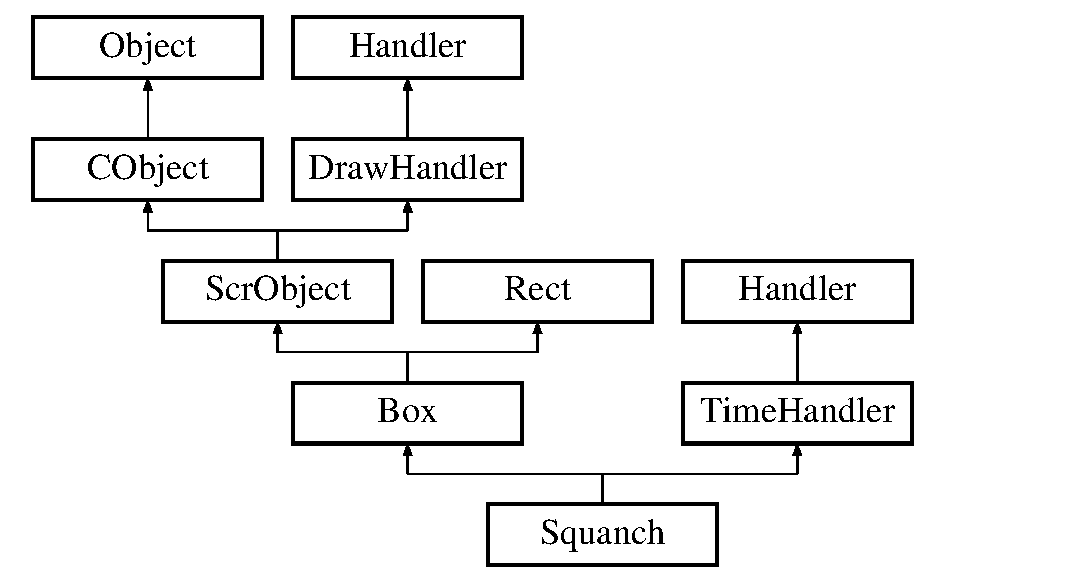
\includegraphics[height=5.000000cm]{class_squanch}
\end{center}
\end{figure}
\subsection*{Public Member Functions}
\begin{DoxyCompactItemize}
\item 
\hypertarget{class_squanch_a6f3df76cfe32e677fdb1c3f4deec2134}{}\label{class_squanch_a6f3df76cfe32e677fdb1c3f4deec2134} 
{\bfseries Squanch} (\hyperlink{class_engine}{Engine} $\ast$game)
\item 
\hypertarget{class_squanch_aecdaa05a52fccbab36eee1702551901e}{}\label{class_squanch_aecdaa05a52fccbab36eee1702551901e} 
void {\bfseries Time\+Event} (double time)
\end{DoxyCompactItemize}
\subsection*{Public Attributes}
\begin{DoxyCompactItemize}
\item 
\hypertarget{class_squanch_a2421d90cee721efa94fce63a881aef5c}{}\label{class_squanch_a2421d90cee721efa94fce63a881aef5c} 
\hyperlink{class_triangle}{Triangle} {\bfseries s\+Quanch}
\item 
\hypertarget{class_squanch_ada1a0d7bb3d52fa9c43515d9a6a19322}{}\label{class_squanch_ada1a0d7bb3d52fa9c43515d9a6a19322} 
\hyperlink{class_square}{Square} {\bfseries sq\+Uanch}
\item 
\hypertarget{class_squanch_a782c18e8f235d328fbca1a67f2565cb6}{}\label{class_squanch_a782c18e8f235d328fbca1a67f2565cb6} 
\hyperlink{class_fancy_square}{Fancy\+Square} {\bfseries bloob}
\end{DoxyCompactItemize}


The documentation for this class was generated from the following file\+:\begin{DoxyCompactItemize}
\item 
Fight\+Game.\+cpp\end{DoxyCompactItemize}

\hypertarget{class_square}{}\section{Square Class Reference}
\label{class_square}\index{Square@{Square}}


Low-\/level \hyperlink{class_object}{Object} prefab that draws a simple colored square.  




{\ttfamily \#include $<$Shape.\+h$>$}

Inheritance diagram for Square\+:\begin{figure}[H]
\begin{center}
\leavevmode
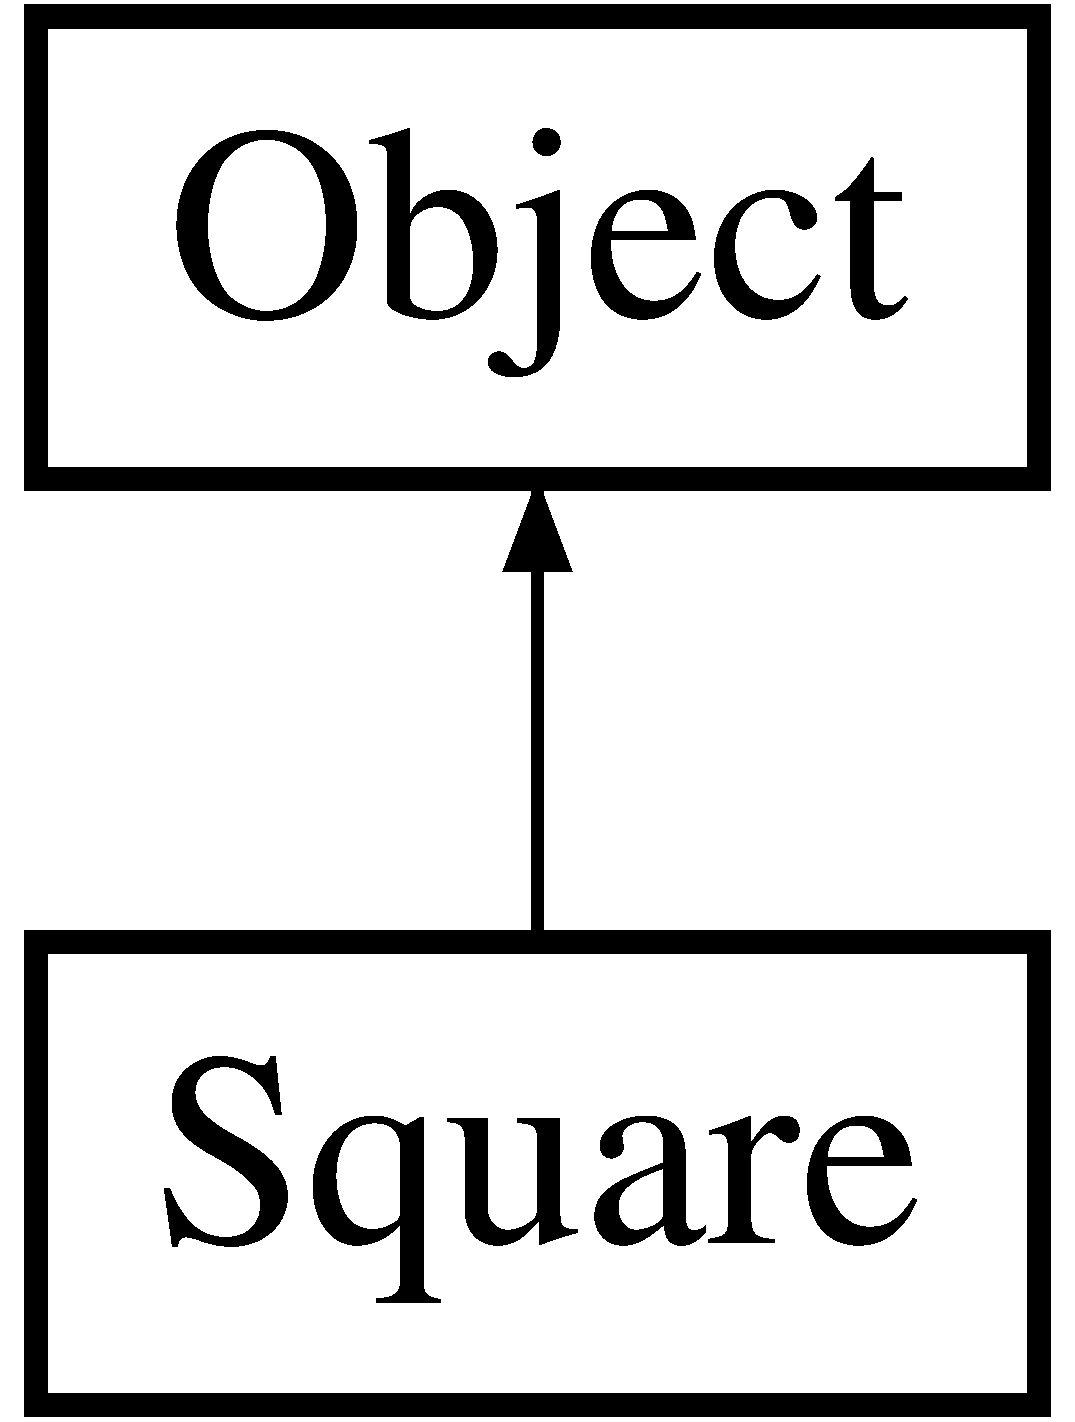
\includegraphics[height=2.000000cm]{class_square}
\end{center}
\end{figure}
\subsection*{Public Member Functions}
\begin{DoxyCompactItemize}
\item 
virtual void \hyperlink{class_square_a9a533e0dd001a0b883bea5145c7444e0}{Draw} (class \hyperlink{class_engine}{Engine} $\ast$game\+Engine, \hyperlink{class_transform}{Transform} parent\+Trans)
\begin{DoxyCompactList}\small\item\em Virtual function meant to be implemented by children. Some objects use Draw to pass information, delegating the actual drawing to the objects at the end of the parent-\/child hierarchy. \end{DoxyCompactList}\end{DoxyCompactItemize}
\subsection*{Public Attributes}
\begin{DoxyCompactItemize}
\item 
\hypertarget{class_square_a45f110963e3c27deb64497779f44e7ec}{}\label{class_square_a45f110963e3c27deb64497779f44e7ec} 
\hyperlink{class_split_model}{Split\+Model} {\bfseries my\+Obj}
\end{DoxyCompactItemize}


\subsection{Detailed Description}
Low-\/level \hyperlink{class_object}{Object} prefab that draws a simple colored square. 

\subsection{Member Function Documentation}
\hypertarget{class_square_a9a533e0dd001a0b883bea5145c7444e0}{}\label{class_square_a9a533e0dd001a0b883bea5145c7444e0} 
\index{Square@{Square}!Draw@{Draw}}
\index{Draw@{Draw}!Square@{Square}}
\subsubsection{\texorpdfstring{Draw()}{Draw()}}
{\footnotesize\ttfamily void Square\+::\+Draw (\begin{DoxyParamCaption}\item[{class \hyperlink{class_engine}{Engine} $\ast$}]{game\+Engine,  }\item[{\hyperlink{class_transform}{Transform}}]{parent\+Trans }\end{DoxyParamCaption})\hspace{0.3cm}{\ttfamily [virtual]}}



Virtual function meant to be implemented by children. Some objects use Draw to pass information, delegating the actual drawing to the objects at the end of the parent-\/child hierarchy. 


\begin{DoxyParams}{Parameters}
{\em game\+Engine} & -\/ Pointer to the game engine that will render this \\
\hline
{\em parent\+Trans} & -\/ \hyperlink{class_transform}{Transform} being passed to the object. With long chains of object children/parents, transforms can be cumulative. \\
\hline
\end{DoxyParams}


Implements \hyperlink{class_object_adeb7a19aaca51dbf093b37fd21c5e41f}{Object}.



The documentation for this class was generated from the following files\+:\begin{DoxyCompactItemize}
\item 
Shape.\+h\item 
Shape.\+cpp\end{DoxyCompactItemize}

\hypertarget{structstbi__io__callbacks}{}\section{stbi\+\_\+io\+\_\+callbacks Struct Reference}
\label{structstbi__io__callbacks}\index{stbi\+\_\+io\+\_\+callbacks@{stbi\+\_\+io\+\_\+callbacks}}
\subsection*{Public Attributes}
\begin{DoxyCompactItemize}
\item 
\hypertarget{structstbi__io__callbacks_a623e46b3a2a019611601409926283a88}{}\label{structstbi__io__callbacks_a623e46b3a2a019611601409926283a88} 
int($\ast$ {\bfseries read} )(void $\ast$user, char $\ast$data, int size)
\item 
\hypertarget{structstbi__io__callbacks_a257aac5480a90a6c4b8fbe86c1b01068}{}\label{structstbi__io__callbacks_a257aac5480a90a6c4b8fbe86c1b01068} 
void($\ast$ {\bfseries skip} )(void $\ast$user, int n)
\item 
\hypertarget{structstbi__io__callbacks_a319639db2f76e715eed7a7a974136832}{}\label{structstbi__io__callbacks_a319639db2f76e715eed7a7a974136832} 
int($\ast$ {\bfseries eof} )(void $\ast$user)
\end{DoxyCompactItemize}


The documentation for this struct was generated from the following file\+:\begin{DoxyCompactItemize}
\item 
stb\+\_\+image.\+h\end{DoxyCompactItemize}

\hypertarget{class_time_handler}{}\section{Time\+Handler Class Reference}
\label{class_time_handler}\index{Time\+Handler@{Time\+Handler}}
Inheritance diagram for Time\+Handler\+:\begin{figure}[H]
\begin{center}
\leavevmode
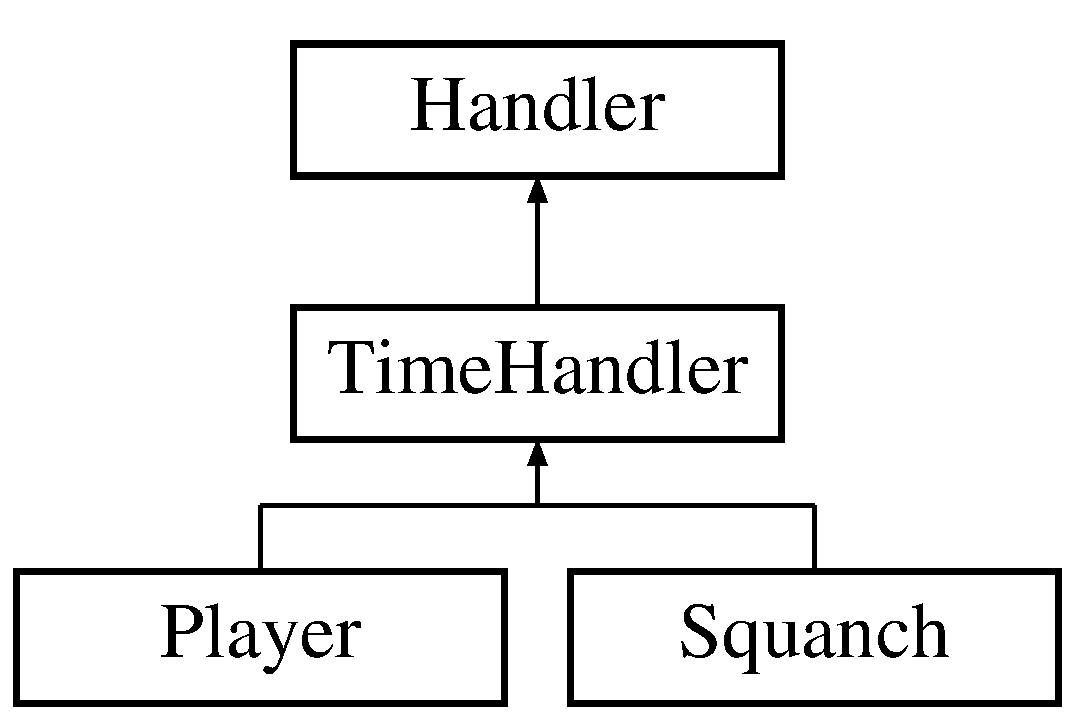
\includegraphics[height=3.000000cm]{class_time_handler}
\end{center}
\end{figure}
\subsection*{Public Member Functions}
\begin{DoxyCompactItemize}
\item 
\hypertarget{class_time_handler_a606ca4ea15838eeed25b77be8c819cf1}{}\label{class_time_handler_a606ca4ea15838eeed25b77be8c819cf1} 
{\bfseries Time\+Handler} (class \hyperlink{class_engine}{Engine} $\ast$game)
\item 
\hypertarget{class_time_handler_aa403cac55724be7af8b790088d40b29c}{}\label{class_time_handler_aa403cac55724be7af8b790088d40b29c} 
virtual void {\bfseries Time\+Event} (double curr\+Time)=0
\end{DoxyCompactItemize}
\subsection*{Additional Inherited Members}


The documentation for this class was generated from the following files\+:\begin{DoxyCompactItemize}
\item 
Handler.\+h\item 
Handler.\+cpp\end{DoxyCompactItemize}

\hypertarget{class_transform}{}\section{Transform Class Reference}
\label{class_transform}\index{Transform@{Transform}}


Class that deals with matrix/vector transformations.  




{\ttfamily \#include $<$Transform.\+h$>$}

Inheritance diagram for Transform\+:\begin{figure}[H]
\begin{center}
\leavevmode
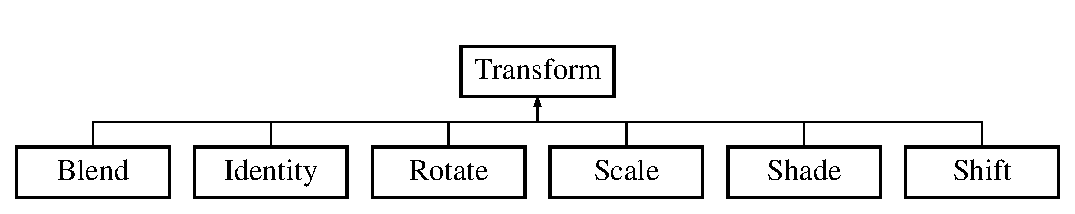
\includegraphics[height=2.000000cm]{class_transform}
\end{center}
\end{figure}
\subsection*{Public Member Functions}
\begin{DoxyCompactItemize}
\item 
\hypertarget{class_transform_ab826e0b6b6a46589e2a8ed4114eae17e}{}\label{class_transform_ab826e0b6b6a46589e2a8ed4114eae17e} 
{\bfseries Transform} (\hyperlink{class_vector}{Vector} X, \hyperlink{class_vector}{Vector} Y, \hyperlink{class_vector}{Vector} Z, \hyperlink{class_vector}{Vector} W, \hyperlink{class_color}{Color} m\+Col, \hyperlink{class_color}{Color} a\+Col)
\item 
\hypertarget{class_transform_a8572d47a093861b3372fe8ee3bddcc10}{}\label{class_transform_a8572d47a093861b3372fe8ee3bddcc10} 
{\bfseries Transform} (const \hyperlink{class_transform}{Transform} \&thing)
\item 
\hypertarget{class_transform_a542213b758a490a2203ea7fd0266776a}{}\label{class_transform_a542213b758a490a2203ea7fd0266776a} 
\hyperlink{class_transform}{Transform} \& {\bfseries operator=} (const \hyperlink{class_transform}{Transform} \&thing)
\item 
\hypertarget{class_transform_ad93311f2830ef5ca081a7d73579d4015}{}\label{class_transform_ad93311f2830ef5ca081a7d73579d4015} 
\hyperlink{class_vector}{Vector} {\bfseries Apply} (const \hyperlink{class_vector}{Vector} \&input)
\item 
\hypertarget{class_transform_a697d100cd8b73be18d5d3af398a0500e}{}\label{class_transform_a697d100cd8b73be18d5d3af398a0500e} 
\hyperlink{class_color}{Color} {\bfseries Apply} (const \hyperlink{class_color}{Color} \&input)
\end{DoxyCompactItemize}
\subsection*{Public Attributes}
\begin{DoxyCompactItemize}
\item 
\hypertarget{class_transform_aa4081baf6061e5f7e54a5c42e416e00e}{}\label{class_transform_aa4081baf6061e5f7e54a5c42e416e00e} 
\hyperlink{class_vector}{Vector} {\bfseries x}
\item 
\hypertarget{class_transform_a3604995547831490d3825b1fe8e1c107}{}\label{class_transform_a3604995547831490d3825b1fe8e1c107} 
\hyperlink{class_vector}{Vector} {\bfseries y}
\item 
\hypertarget{class_transform_ab7412f8029326c0b94c19deb94cf040f}{}\label{class_transform_ab7412f8029326c0b94c19deb94cf040f} 
\hyperlink{class_vector}{Vector} {\bfseries z}
\item 
\hypertarget{class_transform_a2ad38abb95feb341ada8d00b66d67647}{}\label{class_transform_a2ad38abb95feb341ada8d00b66d67647} 
\hyperlink{class_vector}{Vector} {\bfseries w}
\item 
\hypertarget{class_transform_a925437b8247dd58f70fb1b4293d23a69}{}\label{class_transform_a925437b8247dd58f70fb1b4293d23a69} 
\hyperlink{class_color}{Color} {\bfseries mul\+Col}
\item 
\hypertarget{class_transform_ab1127e4bc3d8be4c2396988f703e2648}{}\label{class_transform_ab1127e4bc3d8be4c2396988f703e2648} 
\hyperlink{class_color}{Color} {\bfseries add\+Col}
\end{DoxyCompactItemize}


\subsection{Detailed Description}
Class that deals with matrix/vector transformations. 

\hyperlink{class_transform}{Transform} and its children perform matrix and vertex calculations. Most often, game programmers will make use of the various children to quickly create and pass various kinds of transformations. 

The documentation for this class was generated from the following files\+:\begin{DoxyCompactItemize}
\item 
Transform.\+h\item 
Transform.\+cpp\end{DoxyCompactItemize}

\hypertarget{class_triangle}{}\section{Triangle Class Reference}
\label{class_triangle}\index{Triangle@{Triangle}}
Inheritance diagram for Triangle\+:\begin{figure}[H]
\begin{center}
\leavevmode
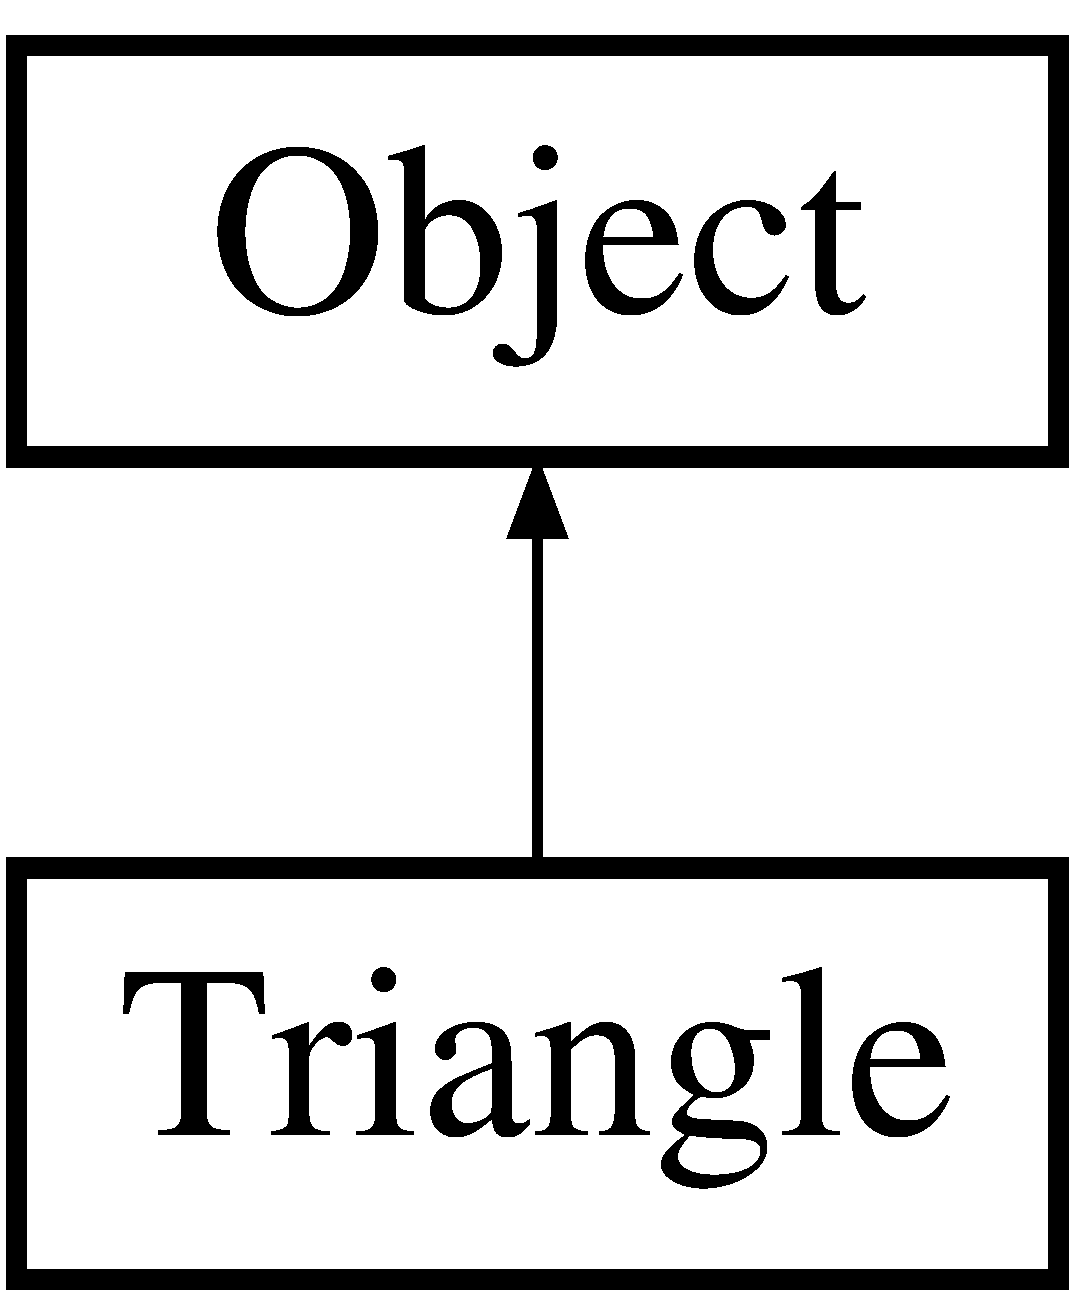
\includegraphics[height=2.000000cm]{class_triangle}
\end{center}
\end{figure}
\subsection*{Public Member Functions}
\begin{DoxyCompactItemize}
\item 
virtual void \hyperlink{class_triangle_a2c8418bbe7a955b9ad53571a5832e1b0}{Draw} (class \hyperlink{class_engine}{Engine} $\ast$game\+Engine, \hyperlink{class_transform}{Transform} parent\+Trans)
\begin{DoxyCompactList}\small\item\em Virtual function meant to be implemented by children. Some objects use Draw to pass information, delegating the actual drawing to the objects at the end of the parent-\/child hierarchy. \end{DoxyCompactList}\end{DoxyCompactItemize}
\subsection*{Public Attributes}
\begin{DoxyCompactItemize}
\item 
\hypertarget{class_triangle_abf0ea31793702554dbc5f446ebb55527}{}\label{class_triangle_abf0ea31793702554dbc5f446ebb55527} 
\hyperlink{class_split_model}{Split\+Model} {\bfseries my\+Obj}
\end{DoxyCompactItemize}


\subsection{Member Function Documentation}
\hypertarget{class_triangle_a2c8418bbe7a955b9ad53571a5832e1b0}{}\label{class_triangle_a2c8418bbe7a955b9ad53571a5832e1b0} 
\index{Triangle@{Triangle}!Draw@{Draw}}
\index{Draw@{Draw}!Triangle@{Triangle}}
\subsubsection{\texorpdfstring{Draw()}{Draw()}}
{\footnotesize\ttfamily void Triangle\+::\+Draw (\begin{DoxyParamCaption}\item[{class \hyperlink{class_engine}{Engine} $\ast$}]{game\+Engine,  }\item[{\hyperlink{class_transform}{Transform}}]{parent\+Trans }\end{DoxyParamCaption})\hspace{0.3cm}{\ttfamily [virtual]}}



Virtual function meant to be implemented by children. Some objects use Draw to pass information, delegating the actual drawing to the objects at the end of the parent-\/child hierarchy. 


\begin{DoxyParams}{Parameters}
{\em game\+Engine} & -\/ Pointer to the game engine that will render this \\
\hline
{\em parent\+Trans} & -\/ \hyperlink{class_transform}{Transform} being passed to the object. With long chains of object children/parents, transforms can be cumulative. \\
\hline
\end{DoxyParams}


Implements \hyperlink{class_object_adeb7a19aaca51dbf093b37fd21c5e41f}{Object}.



The documentation for this class was generated from the following files\+:\begin{DoxyCompactItemize}
\item 
Shape.\+h\item 
Shape.\+cpp\end{DoxyCompactItemize}

\hypertarget{class_vector}{}\section{Vector Class Reference}
\label{class_vector}\index{Vector@{Vector}}
\subsection*{Public Member Functions}
\begin{DoxyCompactItemize}
\item 
\hypertarget{class_vector_a8a3ea7beb7d5c4ecbe92980a408dbe65}{}\label{class_vector_a8a3ea7beb7d5c4ecbe92980a408dbe65} 
{\bfseries Vector} (double X, double Y, double Z)
\item 
\hypertarget{class_vector_a3eada6cc519cbda30dc7addcd4b06854}{}\label{class_vector_a3eada6cc519cbda30dc7addcd4b06854} 
{\bfseries Vector} (const \hyperlink{class_vector}{Vector} \&thing)
\item 
\hypertarget{class_vector_a1f1f32870831166d91f196d6afc2174f}{}\label{class_vector_a1f1f32870831166d91f196d6afc2174f} 
\hyperlink{class_vector}{Vector} \& {\bfseries operator=} (const \hyperlink{class_vector}{Vector} \&thing)
\end{DoxyCompactItemize}
\subsection*{Public Attributes}
\begin{DoxyCompactItemize}
\item 
\hypertarget{class_vector_a133722e00601091cb2075219da5da6e4}{}\label{class_vector_a133722e00601091cb2075219da5da6e4} 
double {\bfseries x}
\item 
\hypertarget{class_vector_a09a21a140718f234eea348d5058cee0b}{}\label{class_vector_a09a21a140718f234eea348d5058cee0b} 
double {\bfseries y}
\item 
\hypertarget{class_vector_a1b604d674485316754b72494f5fcc960}{}\label{class_vector_a1b604d674485316754b72494f5fcc960} 
double {\bfseries z}
\end{DoxyCompactItemize}


The documentation for this class was generated from the following files\+:\begin{DoxyCompactItemize}
\item 
Vector.\+h\item 
Vector.\+cpp\end{DoxyCompactItemize}

\hypertarget{class_vector2}{}\section{Vector2 Class Reference}
\label{class_vector2}\index{Vector2@{Vector2}}
\subsection*{Public Member Functions}
\begin{DoxyCompactItemize}
\item 
\hypertarget{class_vector2_ac01321dfaedc450692fecd7d6ddc1e4b}{}\label{class_vector2_ac01321dfaedc450692fecd7d6ddc1e4b} 
{\bfseries Vector2} (double X, double Y)
\item 
\hypertarget{class_vector2_a69d361c3d08e85232ac94c23988d35b7}{}\label{class_vector2_a69d361c3d08e85232ac94c23988d35b7} 
{\bfseries Vector2} (const \hyperlink{class_vector2}{Vector2} \&thing)
\item 
\hypertarget{class_vector2_a9108dc287c782b035ea9ea854aa945e2}{}\label{class_vector2_a9108dc287c782b035ea9ea854aa945e2} 
\hyperlink{class_vector2}{Vector2} \& {\bfseries operator=} (const \hyperlink{class_vector2}{Vector2} \&thing)
\end{DoxyCompactItemize}
\subsection*{Public Attributes}
\begin{DoxyCompactItemize}
\item 
\hypertarget{class_vector2_a61d73d9036ccbb3257fbe595c014a1d0}{}\label{class_vector2_a61d73d9036ccbb3257fbe595c014a1d0} 
double {\bfseries x}
\item 
\hypertarget{class_vector2_a4df9b2a8e79e6e30a7a3b34722d8b8b8}{}\label{class_vector2_a4df9b2a8e79e6e30a7a3b34722d8b8b8} 
double {\bfseries y}
\end{DoxyCompactItemize}


The documentation for this class was generated from the following files\+:\begin{DoxyCompactItemize}
\item 
Vector.\+h\item 
Vector.\+cpp\end{DoxyCompactItemize}

%--- End generated contents ---

% Index
\backmatter
\newpage
\phantomsection
\clearemptydoublepage
\addcontentsline{toc}{chapter}{Index}
\printindex

\end{document}
